%% Before beginning to type your dissertation, read the formatting guide, 
%% which can be found at http://grad.msu.edu/etd/docs/formattingguide.pdf
%% Also get the latest version of  msuphddissertation.cls and the template file
%% at http://www.math.msu.edu/~weil/MSU_Ph.D._Dissertation.zip
%% Send questions to weil@math.msu.edu
\documentclass{msuphddissertation}
\usepackage{amssymb, amsmath}
\usepackage{natbib}
%\usepackage{subcaption}
\usepackage{graphicx}
\usepackage{url}
%% Insert packages you wish to use except setspace and subfig. 
%% Those packages are loaded automatically.
%% IMPORTANT: Load only those packages you know you will use.
%% Some packages can cause conflicts resulting in improper formatting.
\author{Elijah K. Lowe} %% Put your name in full as it is officially recognized by Michigan State University here.
\title{Making heads and tails of \textit{Molgula}: Next Generation Sequencing Analysis of Closely related tailed and tail-less Ascidian species} %% Put the title of your dissertation here.
\unit{Computer Science \& Engineering - Doctor of Philosophy} %% Put the name of your degree granting unit here. The complete
%% list of these degree granting units can be found at
%% http://grad.msu.edu/etd/docs/DegreeGrantingUnits.pdf

%% Put additional preamble items here.

%%%%%% LANDSCAPE PAGES  %%%%%%
%% The environment, landscapenum, produces a page in 
%% landscape mode and then rotates the page by 90 degrees 
%% making is readable on a computer screen, and places the page number
%% along the 11 inch side, which is the bottom of the rotated page. 

%%%%%%%%%%%%%%%%%%%%%%%%%%%%
%%%%%%%%  NOTE   %%%%%%%%%%%%%%
%% PREPARING A DISSERTATION WITH THIS CLASS FILE DOES NOT %%%
%% GUARANTEE THAT THE GRADUATE SCHOOL WILL APPROVE IT %%%
%%%%%%%%%%%%%%%%%%%%%%%%%%%%%%%

%%%%%%%%%%%%%%%%%%%%%%%%%%%%%%%%%%
%%%%%%%%%%%% WARNING %%%%%%%%%%%%%%%
%% The Graduate School requires that all text, except superscripts %%
%% and subscripts, but including text in imported %%
%% graphics files be in 12 point. For that reason it's recommended %%
%% that no text be part of any imported files. %%

%% Once your document has been filed with the Graduate School,
%% if you wish to produce a version of it whose subscripts and superscripts
%% are in traditional smaller proportion, remove the "%" sign 
%% in front of following command. 
%\DeclareMathSizes{12}{12}{10}{8}
%% If your document has footnotes, remove the "%" sign 
%% in front of following command. 
\renewcommand{\footnotesize}{\small}
%% To single space your document, remove the 
%% two commands \begin{doublespace}
%% and \end{doublespace} below.

\begin{document}

\maketitlepage %%This command will produce the title page of your thesis.
\begin{abstract}
Tunicates are invertebrate chordates and are the sister group to the vertebrates. Although tunicates have little morphological resemblance to vertebrates in their adult stage, they do share several features in their larval stage: a hollow dorsal neural tube, gill slits, and a post-anal tail, containing a notochord\textemdash a group of cells organized in a rod shaped structure - the key features that classify the phyla. Within the tunicates, several ascidians have undergone tail-loss, and many of them are Molgulidae. Hybrids have been produced through the cross fertilization of two \textit{Molgula} species (\textit{Molgula occulta} and \textit{Molgula oculata}), and no other solitary \textit{Molgula} species have been known to hybridize. Here we have sequenced the transcriptomes of several developmental stages of both \textit{M. occulta} and \textit{M. oculata}\textemdash two closely related, free-spawning ascidian species, and their hybrid, in order to study the mechanisms behind tail loss in \textit{M. occulta}. We were first presented with the problem of identifying the best approach for the \textit{de novo} assembly of our transcriptomes. Here we determined that processing reads through digital normalization, a redundancy reduction step, had less of an effect on assemblies than did the assembler used. We then sequenced and assembled the genomes of  \textit{M. occulta}, \textit{M. oculata} and a more distant species, \textit{M. occidentalis}. This allowed us to characterize the genomes, discovering that the species are more divergent then they appear phenotypically, and also supporting better gene models. Through differential expression analysis we determined that \textit{M. oculata} and the hybrid appear to express many shared transcripts that are up-regulated during the formation of the ascidian tail, and that these genes are primarily upregulated in the tailed species and hybrid in relation to the tail-less species. Furthermore, of those transcripts upregulated at the tailbud stage in the hybrid but not in \textit{M. occulta}, it appears that expression is being restored by the \textit{M. oculata} allele. This suggests that the relative lack of differential gene expression in the neurula-to-tailbud transition in \textit{M. occulta} is due to loss-of-function of cis-regulatory elements controlling the expression of key genes involved in tail and CNS formation.
\end{abstract}

%% If you wish to have a copyright page, remove the "%" in front of  \begin{copyrt}
%% and remove the "%" in front of \end{copyrt}.
%% The mandatory form of the Copyright will be generated automatically. 
%% A copyright statement is optional.

%\begin{copyrt}
%\end{copyrt}
%% If you wish to have a dedication, remove the "%" in front of
%% \begin{dedication}
%% \end{dedication}
%% A dedication must be single-spaced and 
%% centered on the page.  Both will be done automatically. 

%\begin{dedication}
%\begin{center} 

%\end{center}
%\end{dedication}

%% If you wish to have an acknowledgment, remove the "%" in front of  \begin{acknowledgment}
%% and remove the "%" in front of  \end{acknowledgment}  
\begin{acknowledgment}
Where do I begin? I am a summation of all the people that I have come in contact with throughout my life. So, I would like to dedicate this text to some of the most influential people. 

I start with my mother Patricia Lowe who always encouraged me to pursue my wildest dreams. My father William Robertson, who taught me to question the world and to always pay attention to the small things. My brother Fard Lowe, who consistently served as an inspiration to me and was someone I could always count on. To my high school counselor, Kathy Giles-Harris and high school math teacher, Christopher Reese who both saw something special in me, and pushed me to pursue it. 

My brothers from Morehouse\textemdash Terron Ferguson, Ryan Shepard, John-Marcus Philips, Sean Brazier and Kelechi Kalu\textemdash who kept the laughs and good times rolling along my journey. You guys always made me feel cool, even though I'm a science nerd.
  
My MSU family, who are too many to name, but I'll name a few\textemdash my brother and sister, Cameron Khalfani Herman and Neem Serra, my best bud Ruby Carrillo, Dr. Barbara Thelamour, my mentor Judi Brown-Clarke, my problem solvers Connie James and Darcie Zubek, Carmel Martin-Fairey, Daniel Couvrtier, Luis Zaman, Chad Byers, Temple Smith, James Kremer, okay I said a few, so I'll stop there. I needed you all along the way, through late nights of studying, endless laughs, awesome food, much needed pep talks and just being there to help me survive Michigan.

Collaborators and friends, Billie Swalla, her lab, Lionel Christiaen, his lab, Alberto Stolfi and the wonderful Princess Claudia Racioppi, who all helped me to develop as biologist, experimentally and conceptually, and who advised me along the way. I look forward to working with you all for years to come. And a special thanks to Billie without whom this project would not exist. We have traveled the world together (well at least a good part of the US and Europe), and done what I think is some good science together.

My advisor, Titus Brown. I cannot thank you enough for guiding me along the way. I truly lucked out when I landed in your lab. You are a great scientist, adviser, mentor, and person, and this is the only time you'll hear (or more like read) me say this.

My awesome committee\textemdash David Arnosti, Jin Chen, Ian Dworkin, and Yanni Sun\textemdash who were always tough, but fair.

And to those who pursue knowledge not for the sake of notability but just to make the world a better place.

\end{acknowledgment}

%% If you wish to have a preface, remove the "%" in front of  \begin{preface}
%% and remove the "%" in front of  \end{preface}  
%\begin{preface}
%% Type your acknowledgment here. An acknowledgment is optional.
%\end{preface}

\TOC

%% If your document contains tables, remove the "%" in front of 
%%  the following line.
\LOT

%% If your document contains figures, remove the "%" in front of
%% the following line.
\LOF

%% If any of your figures contain color, you must
%% include the following disclaimer in the caption of your first figure.
%% "For interpretation of the references to color in this and all other figures, 
%% the reader is referred to the electronic version of this dissertation."

%%%% LIST OF SYMBOLS AND ABBREVIATIONS %%%%
%% Such a list is possible using the environment
%% abbreviationskey
%% here. The list will be included in the TOC as
%% KEY TO SYMBOLS AND ABBREVIATIONS
%%%%%%%%%%

\newpage
\pagenumbering{arabic}
\begin{doublespace}

%% Put the body of your dissertation here. 
%% DO NOT include  the bibliography

\chapter{Introduction}
The origin of body plans is an age-old question. Chordates are distinguished by their body plan: most chordates form tadpole-shaped larvae that commonly have a hollow dorsal neural tube and a post-anal tail containing a central notochord flanked by bilateral muscle \cite{nishida_cell_2014}. During embryogenesis, the notochord serves as the source of a patterning signal for neural tube and paraxial mesoderm, an addition to the axial skeleton for the larval tail \cite{jeffery_evolution_1999,stemple_structure_2005}. Tunicates are one of the three subphyla of chordates and are so grouped because of their outer covering known as a tunic, and during development form the typical tadpole larval body plan \cite{huber_evolution_2000}. Ascidians and larvaceans are two of the groups within the Tunicates, and both develop typical chordate body plans. The ascidians exhibit their tailed body form during their larvae free-swimming stage, using the tail for locomotion  before becoming sessile, undergoing metamorphosis and filter feeding for the remainder of their lives. During the free-swimming larval stage, the elongation and mobility of the tail is dependent upon the proper formation of the notochord and muscle cells \cite{satoh_ascidian_2003}. In ascidians and in lower vertebrates the improper formation of the notochord leads to severely shortened larva that cannot swim or feed properly \cite{di_gregorio_tail_2002,jiang_ascidian_2005,stemple_structure_2005}. Out of  \mytilde3000 ascidian species, 16 are known to have independently lost their larval tail, differentiated notochord, muscle cell, and other chordate features, changing their developmental body plan. The majority of these losses have happened within the \textit{Molgula} clade \cite{berrill_studies_1931,swalla_interspecific_1990}, although the Styelidae also have two identified tail-less species \cite{huber_evolution_2000}.

Ascidians are a simple system in which to study developmental processes: their cell lineages have been traced starting at fertilization \cite{nishida_cell_1983} to gastrulation \cite{nishida_cell_1985,nishida_cell_1987}, they have invariant early cell lineages and a small number of cells \cite{lemaire_evolutionary_2011}, and there has been no documentation of ascidians developing without an invariant cell lineage.  Ascidian development is nearly identical across distantly related solitary ascidians \cite{lemaire_ascidians_2008,nishida_cell_2014}. They also have rapid embryogenesis, compact genomes, and simplified larval body plans containing few larval tissue types \cite{corbo_characterization_1997,jeffery_minireview_2002,dehal_draft_2002}.  %In \textit{Ciona intestinalis} there are ~2,600 cells, with 36 muscle cells and 40 notochord and the time line \cite{}. 
In addition to the several Molgulids that have independently lost their tail, two Molgulids, one tailed and one tail-less species, can be hybridized, offering the opportunity to study the mechanism behind evolutionarily divergent body plans \cite{jeffery_evolutionary_1991}. %Although \textit{M. occulta} and \textit{M. oculata} present great systems evolutionarily to study tail development and loss, they have several shortcomings as experimental models: they are only found on the Northern coast of France and have yet to be cultured, they only spawn for one month out of the year, and many of the molecular techniques used in other ascidians have not yet been optimized for these two species. Thus tunicates are good models for studying notochord specification.

Many genes in the notochord gene network have been identified by subtractive hybridization screening and microarrays \cite{jeffery_factors_1992,hotta_characterization_2000,gyoja_analysis_2007,kobayashi_differential_2013}. More recently, sequencing technologies such as Ion Torrent, Roche 454 and Illumina have made genome or transcriptome wide analysis more readily available for non-model species. These technologies have several advantages over microarrays: they have a wider scope, are more precise and are able to find novel genes \cite{marioni_rna-seq:_2008}. With the advances in technology we have now sequenced the transcriptomes of both species and their hybrid. This ability to sequence the entire transcriptome at a high resolution allows us to look at pivotal time points in tail development and compare across closely related species to identify and study mechanisms that have been lost or modified during evolution. 

We present a comparative study of the tailed \textit{M. oculata} and the tail-less \textit{M. occulta} through gene expression in order to understand the underlying factors behind tail development, tail loss and the origin of the chordate body plan. Although this study presents the first assembled \textit{Molgula} genomes, there are a number of sequenced tunicate genomes available: in particular, we use the assembled and annotated genome of \textit{Ciona intestinalis}, which serves as the most documented and closest complete reference for the \textit{Molgula} and other ascidian species \cite{dehal_draft_2002,satoh_ascidian_2003,satoh_ciona_2003}. We began this project with RNA-seq data from several time points from each of the species (\textit{M. occulta} and \textit{M. oculata}) and their hybrid. 
%Next-generation sequencing (NGS) is an effective method of producing observations and generating hypotheses to be tested experimentally.
Whole genome and transcriptome sequencing will not definitively identify the factors involved in the development of the tailed chordate body plan since other processes are occurring, but examining the correlation of gene expression patterns between the tailed, tail-less and interspecific \textit{Molgula} hybrid allows us to filter genes associated with this process. Before we can make biological inferences from our data we have to produce a quality assembly, and because of this we first assessed the quality of an efficient low-memory assembly pipeline for our RNA-seq data.
%and identified quality metrics other than N50 and contig length, since these are not best metrics for assessing transcriptome quality \cite{oneil_assessing_2013}.
We later obtained genomic DNA and assembled the genomes of \textit{M. occulta}, \textit{M. oculata} and a more divergent species \textit{M. occidentalis}. This allowed us to analyze the homology between ascidian gene networks, and build more complete transcript modules for differential expression \cite{vijay_challenges_2012}.


\chapter{Literature Review}
\section{Ascidian tail development}

The notochord is one of the distinguishing characteristics of chordates: it is responsible for the extension of the larval tail which is typical for chordate body plan. In their adult forms, ascidians and their vertebrate cousins bear little resemblance to one another, however during development they have similar body plans that include the notochord \cite{jeffery_minireview_2002}. Ascidians are known for their bilateral and invariant cell cleavage, and their development is well described up to the gastrulation stage \cite{nishida_cell_1983,nishida_cell_1985,nishida_cell_1987}. Like vertebrates such as Xenopus, ascidians depend on maternally localized determinants to regulate cell moments and division, but while the development of the early body plans are similar the location and identity of these determinants are different \cite{lemaire_ascidians_2008}. Solitary ascidian notochords typically originate from two cell lineages, with the primary notochord deriving from the ``A'' blastomere and the secondary notochord deriving from the ``B'' blastomere \cite{nishida_cell_1983}.  Both ``A'' and ``B'' blastomeres can be identified at the 4-cell embryonic stage. At this stage the blastomeres are labeled according to the Conklin convention: ``a'' and ``A'' label the anterior animal and vegetal blastomeres, while ``b'' and ``B'' label the posterior animal and vegetal blastomeres \cite{conklin_organization_1905} . Although the notochords cells have been traced back to the 4-cell stage, notochord induction does not occur until the 32-cell stage. By the 64-cell stage there are 10 notochord cell precursors, the 8 primary precursor notochord cells\textemdash A lineage\textemdash which are no longer multipotent, and the 2 secondary notochord cells which are not restricted until the 110-cell stage \cite{nishida_cell_1985,yasuo_ascidian_1994,yasuo_conservation_1998,lemaire_unfolding_2009}. Two additional stages of cell division occur, one at gastrulation and one at neurulation, ending with the 40 notochord cells that are typical of most solitary ascidian tadpole larvae \cite{conklin_organization_1905}. At the onset of neurulation the notochord begins to form, a process that includes the closing of the neural tube and posterior movement of the notochord and muscle cells, followed by the mediolateral convergence of the notochord cells to the midline and then the polarization and intercalation of the cells through a process known as convergence and extension\cite{swalla_mechanisms_1993}. At this point the larval tail is constructed of a notochord flanked by 3 rows of muscles on each side, and both notochord and muscle cell derive from the same blastomeres \cite{nishida_cell_1985}. While the arrangement of the notochord cells is a stochastic process, the anterior 32-cells\textemdash primary notochord cells\textemdash are always formed by the A7.3 and A7.7 blastomere and the posterior most 8\textemdash secondary\textemdash notochord cells are always formed by the B8.6 blastomere; however, the ordering of the 32 most anterior is not determinate, in that cells from both the A7.3 and A7.7 intercalate in a random order (Figure~\ref{fig:noto_cells})\cite{nishida_cell_1983,nishida_cell_1985,miyamoto_formation_1985, swalla_mechanisms_1993,kourakis_one-dimensional_2014}. This process, along with muscle cell development, drives the formation of the larval tail \cite{miyamoto_formation_1985, jeffery_factors_1992,swalla_mechanisms_1993}.
\begin{figure}[tbp]
\centering
\includegraphics[scale=0.5]{figures/phylogeny.pdf}
\caption{\textbf{Phylographic sketch.} Phylogenetic placement of Cnidaria and the Bilateria (Protostomata and Deuterostoma). Deuterostomes, which in Greek means second mouth, are distinguished in the Bilateria by forming their anus first. Tunicata and Cephalochordata are the sister groups to Vertebrata. This subphyla shares several characteristics; a notochord, a hollow dorsal nerve cord, and a post-anal tail at some point in their life cycles. (Blue) branches are Deuterostomes. For interpretation of the references to color in this and all other figures, the reader is referred to the electronic version of this dissertation.}
\label{fig:phylog}
\end{figure}

\begin{figure}[thbp]
\centering
\includegraphics[scale=0.5]{figures/noto_cells.pdf}
\caption{\textbf{Notochord cells.}The primary notochord cells (red), also known as the A-lineage, are specified at the 64-cell stage. There are a total of 32 primary notochord cells that come from the A7.3 and A7.7 blastomere, and the intercalation of the cells happen in a stochastic manner. The secondary notochord cells (blue) derive from the B8.6 blastomere and are specified at the 110-cell stage, one cell division after the primary notochord cells.}
\label{fig:noto_cells}
\end{figure}

The ascidian tail is used for dispersal during the free-swimming larval stage, where the ascidian locates a substrate to attach. After becoming sessile the ascidian tail is absorbed into the trunk region, undergoing metamorphosis and filter feeding for the duration of their adult life. Although a tailed larvae is typical of most ascidians, several species within the Stolidobranchia order have individually undergone tail-loss, and many of these species fall in the family Molgulidae \cite{berrill_studies_1931, jeffery_evolution_1999, huber_evolution_2000, maliska_molgula_2010}. Species without tails tend to have lower speciation rates and smaller geographical ranges \cite{maliska_developmental_2013}. The tail-less\textemdash anural\textemdash species develop in a similar manner and are indistinguishable from their tailed\textemdash urodele\textemdash counterparts up to late gastrulation \cite{berrill_studies_1931, swalla_interspecific_1990, jeffery_factors_1992}. This was not the case when studying the indirect and direct developing sea urchins, \textit{Heliocidaris tuberculata} and \textit{Heliocidaris erythrogramma}. \textit{H. erythrogramma} for goes the typical pluteus larval body plan and in doing so changes its developmental plan \cite{henry_evolutionary_1990}. After the 4 cell division an unequal three-tiered cleavage is established in \textit{H. tuberculata} and other indirect developers along with the lost of cell division synchrony. In contrast, in \textit{H. erythrogramma} and other direct developers, blastomeres are equivalently sized, cleavage orientation remains parallel and cell division is synchronous. Cell fates also differs between direct and indirect sea urchin species \cite{wray_evolutionary_1989}. The change in body plan in Molgula is a much more recent evolutionary occurrence and gives insight on to early onsite of changing body plans, alternative methods outside of change of cell fate and the ancestral chordate body plan.  

Anural ascidians lack several urodele features including an intercalated and extended notochord, differentiated muscle cells and the otolith sensory organ. The absence of differentiated muscles cells and intercalated notochord are the likely cause of tail-lessness in these species \cite{miyamoto_formation_1985, swalla_interspecific_1990}. The development of several tail-less species has been studied in some detail. \textit{Molgula tectiformis} notochord cells do not divide again after the 10 precursor cells are formed and \textit{M. occulta} stops dividing after 20 cells \cite{jeffery_evolution_1999}. The same occurs in \textit{M. bleizi}, however after the 20 notochord cells are formed, the embryo attempts to make a tail but never completes the process \cite{swalla_novel_1993}. It has also been shown that chordate embryos without fully developed notochord and/or muscle cells do not fully elongate or fail completely to develop a tail \cite{jeffery_evolution_1999,takada_brachyury_2002,stemple_structure_2005}. 
Vertebrates, cephalochordates and most ascidians have tailed larvae and interspecific \textit{Molgula occulta/oculata} hybrids can restore the urodele features, this is evidence that the ancestral chordate had a tailed larvae and that the mechanism for tail development was present in anural ascidians but was lost over evolutionary time \cite{berrill_studies_1931,jeffery_factors_1992}.

In order to study specific mechanisms of tail loss, we can study closely related anural and urodele species.  One such pair of species, \textit{M. oculata} and \textit{M. occulta}, both of the Roscovita clade, have been shown to produce hybrids in lab conditions. Of the known \textit{Molgula} species \textit{M. occulta} and \textit{M. oculata} are the only two that can hybridize. Although \textit{M. occulta} and \textit{M. oculata} have been found to dwell in the same habitat, hybrids have not been found in nature and have only been produced in lab conditions. Fertilizing \textit{M. oculata} eggs with \textit{M. occulta} sperm in most cases produce embryos with fully formed tails. The reciprocal cross (\textit{M. occulta} eggs X \textit{M. oculata} sperm) produces a hybrid embryo with 20 notochord cells like \textit{M. occulta}, however the notochord cells converge and extend like \textit{M. oculata} \cite{swalla_interspecific_1990}. The ascidian tail has been shown to form in the presence of notochord and the absence of muscles cells \cite{miyamoto_formation_1985}. Tail development is similar in short-tailed hybrids, the notochord is not flanked by muscle as in tailed species and the tail is only as long as the notochord \cite{swalla_novel_1993}. Hybrid embryos that develop urodele features are batch specific, and tails develop only in batches of \textit{M. occulta} eggs that express the \textit{p58} protein which is associated with cytoskeleton \cite{swalla_identification_1991,jeffery_factors_1992}. Additionally, in hybrid embryos in which urodele features are restored, the number of cells that express acetylcholinesterase (AChE) in a vestigial muscle cell lineage increased in comparison to hybrids lacking urodele features and \textit{M. occulta} \cite{jeffery_evolutionary_1991}. This along with evidence that the ancestral notochord\textemdash the axochord\textemdash is muscle based \cite{lauri_development_2014}, suggests the need for both notochord and muscles cell lineages for the formation of the ascidian tail. 

\section{Notochord development as seen through \textit{Brachyury}}

\textit{Brachyury}, a T-box transcription factor, has been identified as essential for notochord development \cite{yasuo_conservation_1998}. \textit{Bra} was first discovered in mouse, where heterozygotes develop with shorten tails, and homozygotes fail to form a tail and die in utero \cite{herrmann_t_1994}. The notochord is induced by {\em bra} in both vertebrates and ascidians, with consistent timing and location expression of \textit{bra} in the notochord and mesoderm of mouse, xenopus, zebrafish and chicken \cite{kavka_tales_1997}, although {\em bra} is expressed exclusively in the notochord cells in ascidians \cite{yasuo_ascidian_1994}. Notochord induction is regulated by the \textit{FGF/MAPK/Ets} signaling cascade \cite{minokawa_binary_2001}. In particular, the A6.2 and A6.4 notochord/nerve cord precursors are induced by \textit{FGF9/16/20} at the 32-cell stage, just after the 7th cell cleavage \cite{satoh_ascidian_2001}. It was observed from isolation experiments that notochord/nerve cord precursors that lose \textit{FGF9/16/20} competence at the 32-cell stage assume the default nerve cord cell fate, but the converse is true for presumptive nerve cord blastomeres that are introduce to \textit{FGF}: they forgo their default nerve cord fate and become notochord \cite{yasuo_conservation_1998,minokawa_binary_2001}. If \textit{FGF9/16/20} is not present at the 32 cell stage competence is lost, \textit{bra} is not induced and the notochord no longer forms \cite{nakatani_basic_1996,nakatani_duration_1999}. This is because \textit{MAPK} is not activated and the induction of \textit{bra} and repression of \textit{FoxB} are not carried out \cite{hashimoto_transcription_2011}. Without the repression of \textit{FoxB TF} the notochord cell fate is repressed through the repression of \textit{bra}. It has been observed in \textit{H. roretzi} that \textit{FoxB} represses the activation of \textit{bra} predominately through the binding of Fox BS1 (GCACTGA\textit{ACAAACA}TACATAG). \textit{FoxB} is activated by \textit{ZicN} and is present in both nerve cord and notochords precursors, however it is repressed by \textit{MAPK} in the notochord cell lineage at the 64-cell stage \cite{hashimoto_transcription_2011}. \textit{MAPK} is thought to be repressed by \textit{Ephrin/Eph} signaling which is one of the key differences between notochord and nerve cord determination. \textit{Ephrin} ligand is expressed in the epidermis and signals to the future nerve chord cells, inhibiting \textit{FGF/MAPK} pathway. Notochord cells, not being in contact with the epidermis, are free to activate \textit{FGF/MAPK}, and activate \textit{bra}. At this point \textit{bra} is expressed first weakly in the at the 64-cell stage in the notochord/nerve chord precursors \cite{yasuo_ascidian_1994} and unlike other chordates, in ascidians \textit{bra} is only expressed in the notochord cells \cite{yasuo_function_1993,corbo_characterization_1997,hotta_temporal_1999,takada_brachyury_2002}. Although \textit{bra} is necessary, its presence does not guarantee a tail. \textit{M. occulta} and \textit{M. tectiformis}, two tailless \textit{Molgula}, both express \textit{bra}. In both cases \textit{bra} expression stops earlier than that of \textit{M. oculata}, while notochord development is slightly different between the two species. \textit{Bra} is expressed in the 10 precursor notochord cells in \textit{M. occulta}, which undergo another round of cell division, while this final division does not occur in \textit{M. tectiformis}.  In  both \textit{M. occulta} and \textit{M. tectiformis}, larva-specific muscle actin genes have become pseudogenes, however the mutation in the muscle actin genes are not the same between the two species  \cite{swalla_novel_1993,jeffery_evolution_1999}. \textit{Manx} is another gene identified to be important for tail development in \textit{Molgula}, and while it is lowly expressed in \textit{M. occulta}, it has been shown to restore the hybrid tail \cite{swalla_requirement_1996, swalla_multigene_1999}. 
  
After cell specification, the notochord cells must converge, intercalate and extend. The Planar Cell Polarity (PCP) pathway is involved in cell movement during this process and mutations in \textit{prickle}\textemdash a known PCP gene\textemdash have been shown to cause a shortened ascidian tail by affecting both the mediolateral intercalation and the elongation of the ascidian tail \cite{jiang_ascidian_2005}. The \textit{pk} mutant \textit{aimless} produces a truncated tail, however the polarity of the nuclei is established, showing that prickle does not establish polarity within the cell but polarity between cells, acting in a local manner and perhaps as a global organizer \cite{jiang_ascidian_2005,kourakis_one-dimensional_2014}. However, even in the absence of the PCP pathway considerable convergence and elongation of the notochord was observed in Ciona, driven by a presumed boundary effect \cite{veeman_chongmague_2008}.

Many of the upstream genes and transcription factors that interact with \textit{bra} have been studied in detail, through knock-outs and cell isolation experiments. A larger scale subtractive screening was done to identify genes downstream of \textit{bra}, in which 39 genes were initially found \cite{hotta_temporal_1999}. A number of these genes have been characterized, identifying functions such as extracellular matrix components (\textit{cadherin 8, entactin, fibronectin, laminin $alpha$1, $alpha$4, and $beta$1}, and {\em thrombospondin}), cell shape and polarity (\textit{pk, trop, ERM, ACL}), and axon guidance (\textit{netrin, semaphorin 3A}), amongst a host of other biological processes \cite{hotta_characterization_2000,hotta_brachyury-downstream_2007,kugler_evolutionary_2008}. Additionally, downstream genes regulated by \textit{bra} have been examined by using ChIP-seq to identify many known genes in the network, as well as to discover new genes \cite{kubo_genomic_2010,katikala_functional_2013}.

Larvaceans are pelagic tunicates that also develop in a typical chordate manner, featuring  a notochord. However, larvaceans notochords contain only 20 cells \cite{seo_miniature_2001,denoeud_plasticity_2010}. The larvacean  \textit{Oikopleura dioica} retains its tail during its adult life stage and at this point \textit{bra} is not expressed in the adult notochord, however, \textit{bra} is expressed in the same manner in the developing larval notochord as ascidians \cite{bassham_brachyury_2000,nishida_development_2008}. When comparing gene networks for the extent of variation, \textit{Oikopleura} did not exhibit the same mechanism for tail development as \textit{Ciona}: of the 50 {\em bra} target genes previously identified in \textit{Ciona}, only 26 of them had orthologs in the \textit{Oikopleura} genome, meaning that almost 50\% of candidate bra target  genes are not present \cite{kugler_evolutionary_2011}. Of the genes that did show homology, expression ranged from notochord-specific to tail-general, including expression in possible notochord to tissues that were clearly not the notochord. From this we can infer that additional genes have gained function in notochord formation in the \textit{C. intestinalis} gene regulatory network, and the ancestral tunicate may have had a small core set of genes for notochord formation.

\section{Assembling and analyzing data}

One of the major advances in biological sciences in the past 20 years has been the implementation of sequencing technologies. These technologies allow us to examine biological systems genomically, with increasing ease. The first widespread sequencing technology was Sanger sequencing in the 1986, but Sanger sequencing was not broadly used until 10 years later, when automated sequencers became available. Another technology, microarrays, which became popular starting in the mid '90s, allowed us to look at a wide spectrum of genes and understand relative expression within a sample. For example, Kobayashi et al. \cite{kobayashi_differential_2013} isolated and analyzed gene expression in notochord (A7.3+A7.7) and nerve cord (A7.4+A7.8) precursors using microarrays. This study was able to identify 106 genes expressed in the notochord precursor and 68 expressed in the nerve cord precursor at the 64-cell stage. Of these the genes, 36 notochord genes and 25 nerve chord genes were confirmed via whole mount in situ hybridization in the respective cells. This demonstrates the power of this technique, however, prior knowledge of the gene sequences involved were needed. \textit{C. intestinalis} was sequenced using Sanger sequencing, and is the best assembled and most well annotated ascidian genome \cite{dehal_draft_2002}. In addition to long (Sanger) reads, scaffolding was done using scaffold-joining guided by paired-end expressed sequence tags and bacterial artificial chromosome (BAC) sequences, and BAC chromosomal in situ hybridization data \cite{satou_improved_2008}. Sanger sequencing is able to sequence whole genomes without the need of prior knowledge to identify novel genes but was costly and time consuming\cite{metzker_emerging_2005,liu_comparison_2012}. 

Sanger was the first generation of sequencing technologies, and currently both second and third generation are in use, with Roche 454, Ion Torrent, Illumina and PacBio being the most widespread. These technologies produce data far more easily and at a much lower cost than Sanger sequencing \cite{metzker_emerging_2005}. There are many trade-offs for each of the technologies, including cost per MB, sequencing time, prep cost, error rate and sequencing bias; in particular, 454 and PacBio have longer reads than Illumina and Ion Torrent, 800 bp and 1+kbp, respectively. However, both Illumina and Ion Torrent's short reads are cheaper to generate, produce more reads and are better for digital counting; in addition, PacBio has a very high error rate \cite{glenn_field_2011}. Illumina and Ion Torrent have the lowest error rates and while Ion Torrent is more sensitive to single nucleotide polymorphisms, it also calls many more false positives.  Illumina has become the most used NGS technology because it is the most versatile and performs the best in general \cite{quail_tale_2012}. The associated drop in sequencing price has yielded many of the assembled genomes within the Tunicata phyla. Outside of this project there are ten tunicate genomes assembled; \textit{C. intestinalis} (species ``Type A'' and ``Type B''), \textit{C. savignyi}, \textit{Oikopleura dioica}, \textit{Botryllus schlosseri}, \textit{Halocynthia aurantium}, \textit{H. roretzi}, \textit{Phallusia fumigata}, \textit{P. mammilata}, and \textit{Didemnum vexillum}, but no \textit{Molgula} genomes. Molgula genomes and transcriptomes, specifically the tailed \textit{M. oculata} and the tail-less \textit{M. occulta} would make great systems to study the development of the chordate tail and chordate body plan. 

\chapter{Evaluating a lightweight transcriptome assembly pipeline on two closely related ascidian species}\footnotetext{This chapter is in review at PeerJ: Lowe, Swalla, and Brown, 2014 (\url{http://dx.doi.org/10.7287/peerj.preprints.505v1)}.}

\section{Introduction}

Next generation sequencing (NGS) has allowed us to study organisms with a broader lens, looking at entire genomes and transcriptomes instead of single genes.  This capability is particularly important for non-model organisms where little prior knowledge may be available, and where NGS readily enables whole-transcriptome analyses \citep{wang_rna-seq:_2009}, allowing us to study organisms that are ecologically or evolutionarily interesting.

There are now several sequencing technologies, Illumina being one of the most versatile \citep{glenn_field_2011}, that can produce millions of short reads ranging from 75 to 150 bp in length at a low cost \citep{zhang_impact_2011}. As sequencing costs continue to drop, transcriptomes from multiple developmental stages of non-model organisms can easily be sequenced. Various types of \textit{de novo} assembly algorithms and reference based assembly approaches have been developed to handle this massive influx of transcriptomic data \citep{pop_genome_2009,vinson_assembly_2005,stapley_adaptation_2010}. It has been shown in some cases that mapping mRNA-seq reads to a reference genome yields better transcriptomes than \textit{de novo} assemblies, even if the genome is 5-15\% divergent \citep{vijay_challenges_2012}. However, with many non-model organisms, no closely related reference genome is available.

\textit{De novo} is the only solution for transcriptome assembly of organisms with no evolutionarily close reference genome.  Transcriptome assemblers such as Trinity \citep{grabherr_full-length_2011} and Velvet/Oases \citep{zerbino_velvet:_2008,schulz_oases:_2012} use De Bruijn-graph based \textit{de novo} approaches which build graphs connecting the reads based on k-mer overlap. These graphs are then traversed via an Eulerian path algorithm to assemble transcripts. Because De Bruijn graphs are based on exact matches between DNA words, increasing numbers of sequencing errors result in an exponential number of new paths, adding to the complexity of the graph and, in turn, increasing the assembly time and memory requirements \citep{pop_genome_2009}. This is both time consuming and limits the ability to assembly a transcriptome by the amount of available resources.

Here we have sequenced the transcriptomes of several developmental stages of \textit{Molgula occulta} and \textit{Molgula oculata}\textemdash two closely related, free-spawning ascidian species, with no available reference genome. \textit{Ciona intestinalis} and \textit{Ciona savignyi} are the closest related ascidian species with well-assembled genomes, but are not close enough to use as a nucleotide reference for transcriptome construction. In this paper, we describe an efficient, easy to follow protocol for the transcriptome assembly of two Molgulid developmental transcriptomes. A crucial part of this protocol is the use of a preprocessing step that normalizes read abundances prior to assembly, called ``digital normalization.'' We study the effect of digital normalization on assemblies performed with both Trinity and Velvet/Oases.  We compare our approach to the results of running Trinity and Velvet/Oases without digitally normalized reads and show that our approach recovers 99\% the same gene content but has significantly reduced requirements for time and memory.  This reduction in time and memory lets us assemble transcriptomes efficiently using cloud resources, making our results exceptionally easy to reproduce \citep{haas_novo_2013}, and more broadly enabling transcriptome assembly by researchers without access to large computer resources.

\section{Methods}
\subsection{Sequencing preparation}
\textit{M. occulta} and \textit{M. oculata} were collected by dredging off the shores of Roscoff, France near La Station Biologique. Swalla et al have previously described the maintenance \citep{swalla_interspecific_1990} and culturing \citep{swalla_multigene_1999} of the animals. The transcriptomes of \textit{M. occulta} and \textit{M. oculata} were sequenced at Michigan State University (MSU) in the Research Technology Support Facility on Illumina HiSeq 2000. Five lanes of sequences were generated for \textit{M. occulta}, two lanes of the gastrula stage (F+3), one of neurula (F+4), one of early tailbud (F+5), and one from the tailbud (F+6) stage (Table 1). Three lanes of sequences were generated for \textit{M. oculata}, one each for the gastrula, neurula and tailbud stage. 10$\mu$g of RNA were sequenced for each stage with the exception of \textit{M. occulta} F+4, where 1.05$\mu$g of RNA was sequenced. On average each embryonic stage yielded 48 million reads of 75 base pairs (bp) in length with paired-end insert lengths of 250 bp. All reads can be found in the NCBI short read archive (SRA) under accession number SRP040134. 

\subsection{Assembly protocol}
Below is an overview of the steps used for the \textit{de novo} assembly and annotation of our transcriptomes.
\begin{enumerate}
	\item Quality trimming and filtering of raw reads.
	\item Apply digital normalization to decrease data size.
	\item Assemble transcriptome.
	\item Assess transcriptome quality.
	\item BLAST (gene recovery/identification).
\end{enumerate}
Scripts used to run these steps can be found in the following GitHub repository: \url{https://github.com/ged-lab/2014-mrnaseq-cloud}
\subsection{Pre-assembly read trimming and normalization} 
Low quality bases were trimmed and low quality reads were removed using quality-trim-pe.py found in the scripts directory of the repository. A hard trim is done at a Phred quality score of 33 and reads less than 30 base pairs in length are discarded. This process creates a paired and singleton fastq file for each library because of the removal of low quality reads. The filtering of reads allows for better assembly and better mapping, although it may also reduce sensitivity to low-expressed transcripts \citep{lohse_robina:_2012, macmanes_optimal_2014}. The reads were initially 75 bp long, and the average base pair (bp) length was 63 bp after quality trimming and filtering. After quality trimming reads were either directly assembled, or first preprocessed with digital normalization and then assembled. 

Digital normalization (diginorm) is a technique that down samples reads from highly abundant transcripts while retaining approximately the full sequence information content of the reads \citep{brown_reference-free_2012}. Here, for each species, reads from all stages were normalized together to build a common reference transcriptome; reads were normalized to a k-mer coverage of 20 with the k-mer size set to 20 as well.  The initial data set from \textit{M. occulta} contained 237 million reads from 5 lanes, and \textit{M. oculata} contained 150 million total reads; after digital normalization, the \textit{M. occulta} dataset was reduced to 91.6 million reads and \textit{M. oculata} was reduced to 50 million reads, a ~60\% and ~77\% reduction respectively (Table~\ref{fig:time_and_memory.pdf}).

\begin{table}[ht]
\centering
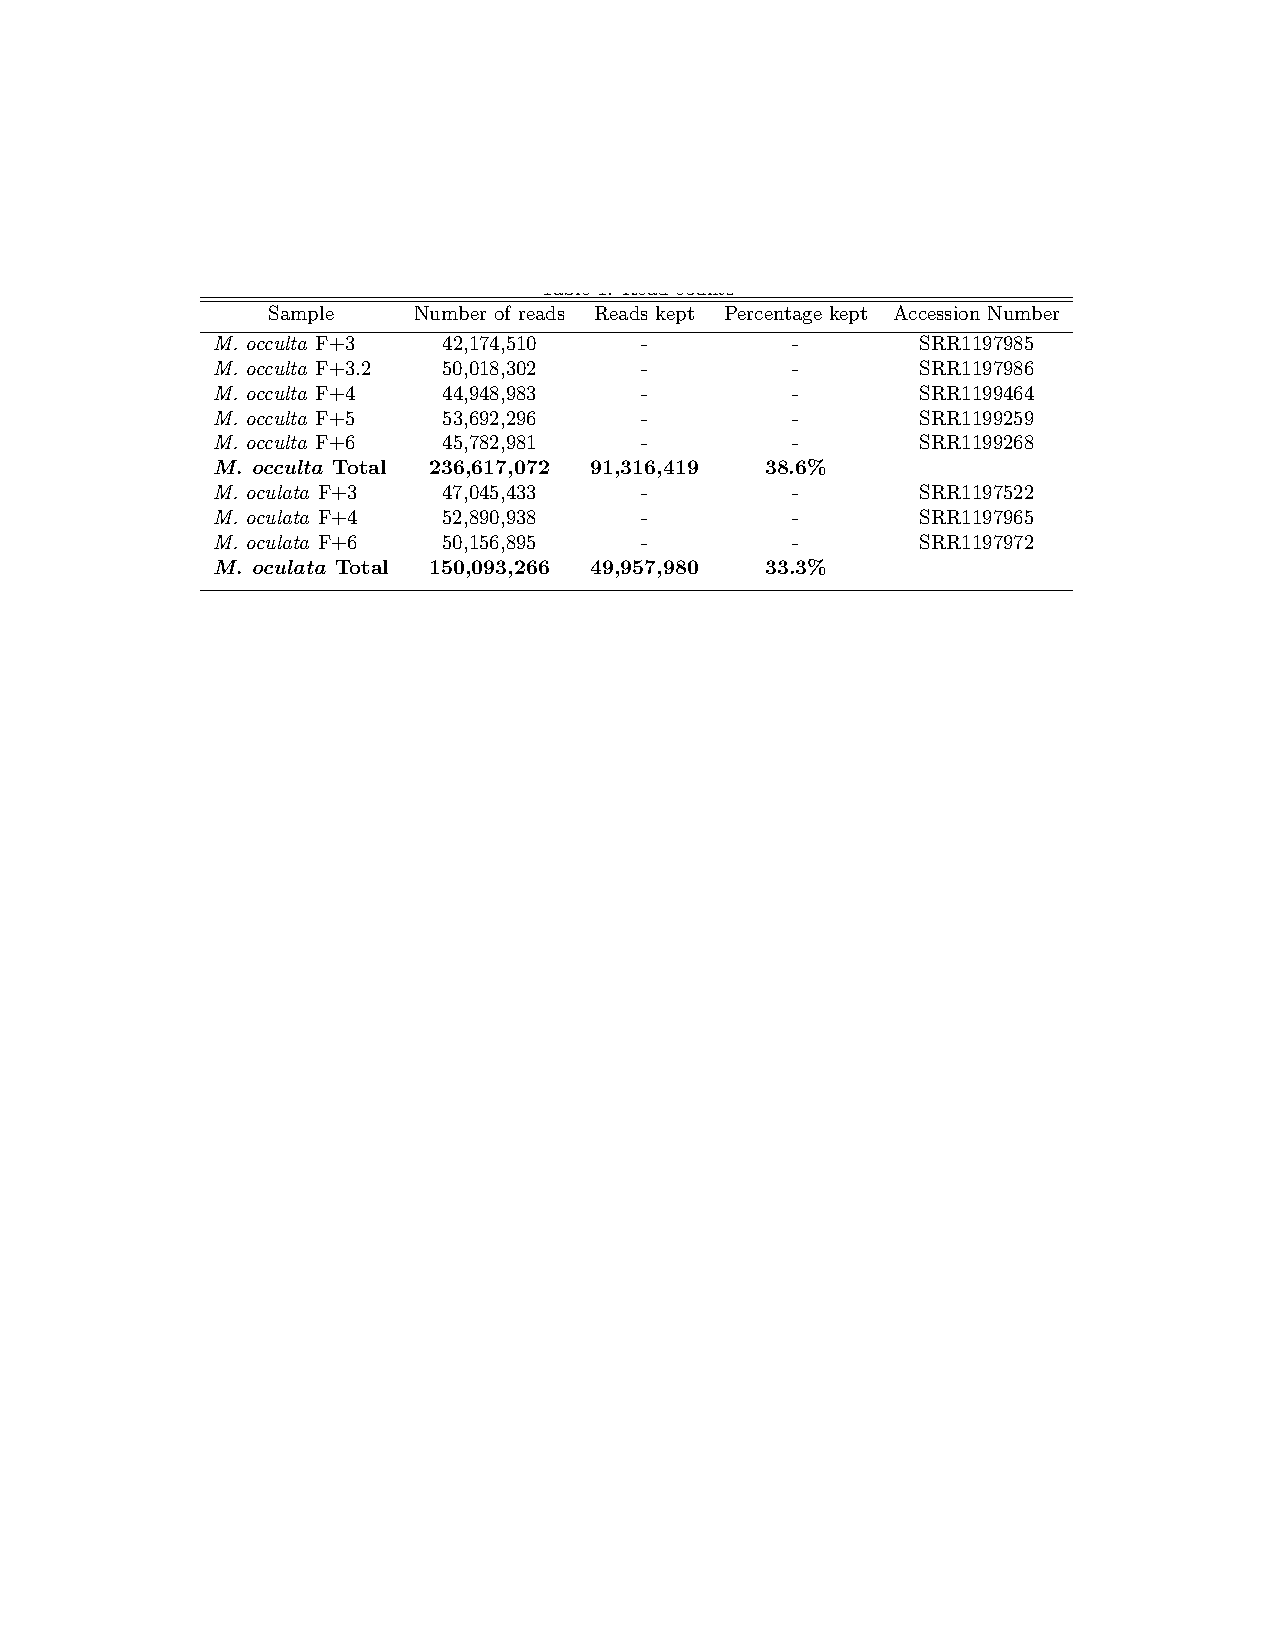
\includegraphics[scale=1.0]{manuscript/Table1.pdf}
\caption{\textbf{Digitally normalized reads.} The number of reads sequenced before and after digital normalization is shown for each lane of sequencing. The percentage of total reads kept after digital normalization is shown in bold. \textit{M. occulta} had approximately \mytilde237 million reads and was reduced to 91 million reads, a 60\% reduction. \textit{M. oculata} had 150 million reads and was reduced by 77\% to \mytilde50 million reads. }
\label{table:Table1.pdf}
\end{table}

\subsection{Transcriptome assembly}
We used the Trinity (r20140413p1) and Velvet/Oases (v1.2.08/v0.2.08) assembler packages, both of which have been broadly used on other data sets \citep{vijay_challenges_2012,grabherr_full-length_2011,schulz_oases:_2012}.  Velvet was initially developed to assemble genomes, and the Oases add-on package was developed for transcriptome assembly, since transcriptomes have variable coverage and many isoforms.  Since Oases cannot be run without Velvet, we refer below to transcriptomes assembled with Velvet and Oases as Oases assemblies. Unlike Trinity, Oases requires the choice of a k-mer overlap for assembly; we chose several k values ranging from k = 21 to k = 35, for odd values of k, with scaffolding turned off. After assembly, the Oases transcriptomes with the highest number of blast hits to \textit{C. intestinalis} were selected for further analysis. The Trinity assembler was run with default parameters.

All assemblies were performed on the Michigan State University (MSU) High Performance computing cluster (HPCC).  All diginorm assemblies were repeated on Amazon EC2 machines as a proof of concept.
After assembly, transcripts shorter than 200 bp in length were removed, and CD-HIT was used to eliminate small transcripts with 99\% identity to longer transcripts using the following command: ``cd-hit-est -i \textless transcript file\textgreater -c 0.99 -o \textless output file\textgreater'' \citep{li_cd-hit:_2006}.

To choose the best k-mer parameter for the Oases assemblies, \textit{C. intestinalis} proteins were searched with TBLASTN (e-value cutoff of 1e-6) against each Oases assembly and the transcriptome with the most hits was selected for further analysis.
\subsection{Gene identification}
We used standalone BLAST to find reciprocal best hits (RBH) between the eight assembled transcriptomes and the \textit{C. intestinalis} proteome retrieved from NCBI under search term ``(ciona intestinalis) AND Ciona intestinalis [porgn:\_\_txid7719]''. At the time of retrieval there were 16,123 sequences and they were downloaded and stored in the GitHub repository under the file name ``ciona\_transcriptome.fa'' in case the sequences change on NCBI. An e-value cutoff of 1e-6 was used as a minimum threshold for transcript identity.  The find-reciprocal-2.py script was used to identify the RBH.
\subsection{Read mapping}
	To determine the inclusion of reads in the various transcriptome assemblies trimmed reads were mapped to their respective species using bowtie2 v2.2.1 \citep{langmead_fast_2012}. For both unnormalized read and diginorm assemblies the full set of trimmed reads were used for mapping. Default parameters were used, and both paired ends and singletons were mapped. Samtools v0.1.19 \citep{li_sequence_2009} was used for format conversion from SAM to BAM format, and also to calculate the percentage of mapped reads. The BAM files were also used to calculate the coverage of transcripts.

\section{Results}

\subsection{Digital normalization reduces the resources needed for assembly}
 The \textit{M. oculata} unnormalized read data set assembled with Oases used 44 CPU hours and 85 GB of RAM. The Oases assembly done with the digitally normalized reads took \mytilde22 CPU hours and 21 GB of RAM (Figure~\ref{subfig-1:figure_1_time}); this includes the time and memory required to run the digital normalization pipeline. \textit{M. occulta} diginorm Oases assembly required over 100 GB of RAM, and the raw read Oases used 300 GB of RAM. The raw read Oases assemblies for both species took twice as long and needed at least three times as much memory when compared to the diginorm reads.

The difference in assembly time and memory between diginorm and raw reads was not as large when using the Trinity assembler. Diginorm completed its assemblies several hours faster than assembling raw reads, \mytilde15 hours compared to \mytilde26 hours for \textit{M. oculata} and \mytilde24 hours compared to \mytilde39 hours for \textit{M. occulta}. \textit{M. oculata} unnormalized reads did not require much more memory than the normalized reads\textemdash 16.8 GB and 15.65 GB, respectively. Diginorm had a larger effect on \textit{M. occulta}, assembling \textit{M. occulta} normalized reads with 23.17 GB of RAM versus 34.14 GB of RAM for the unnormalized reads (Figure~\ref{subfig-2:figure_1_memory}).

\begin{figure}[tbp]
\centering
\subfloat[\textit{Time to complete assemblies}\label{subfig-1:figure_1_time}]{%
	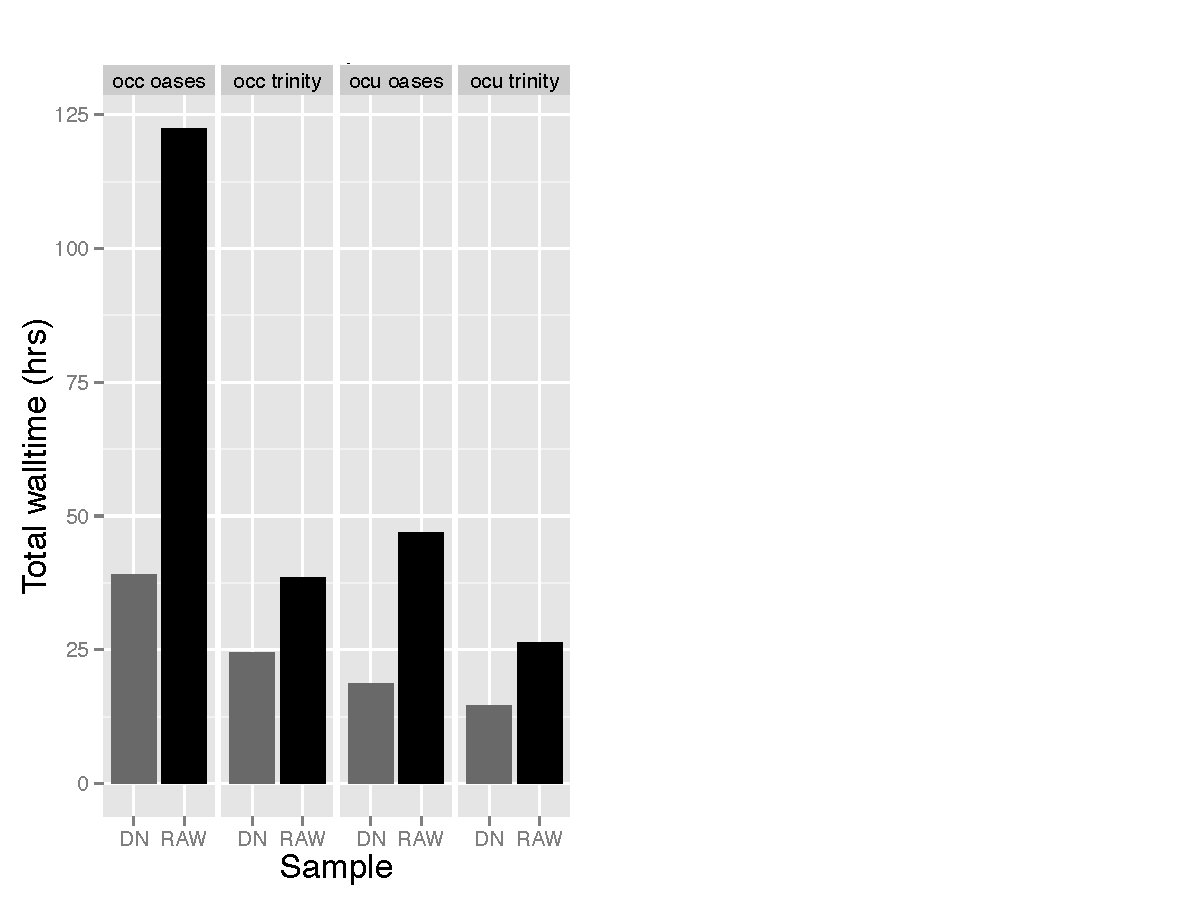
\includegraphics[width=0.45\textwidth]{manuscript/figure_1_time.pdf}
	}
	\hfill
	\subfloat[\textit{Memory to complete assemblies}\label{subfig-2:figure_1_memory}]{%
	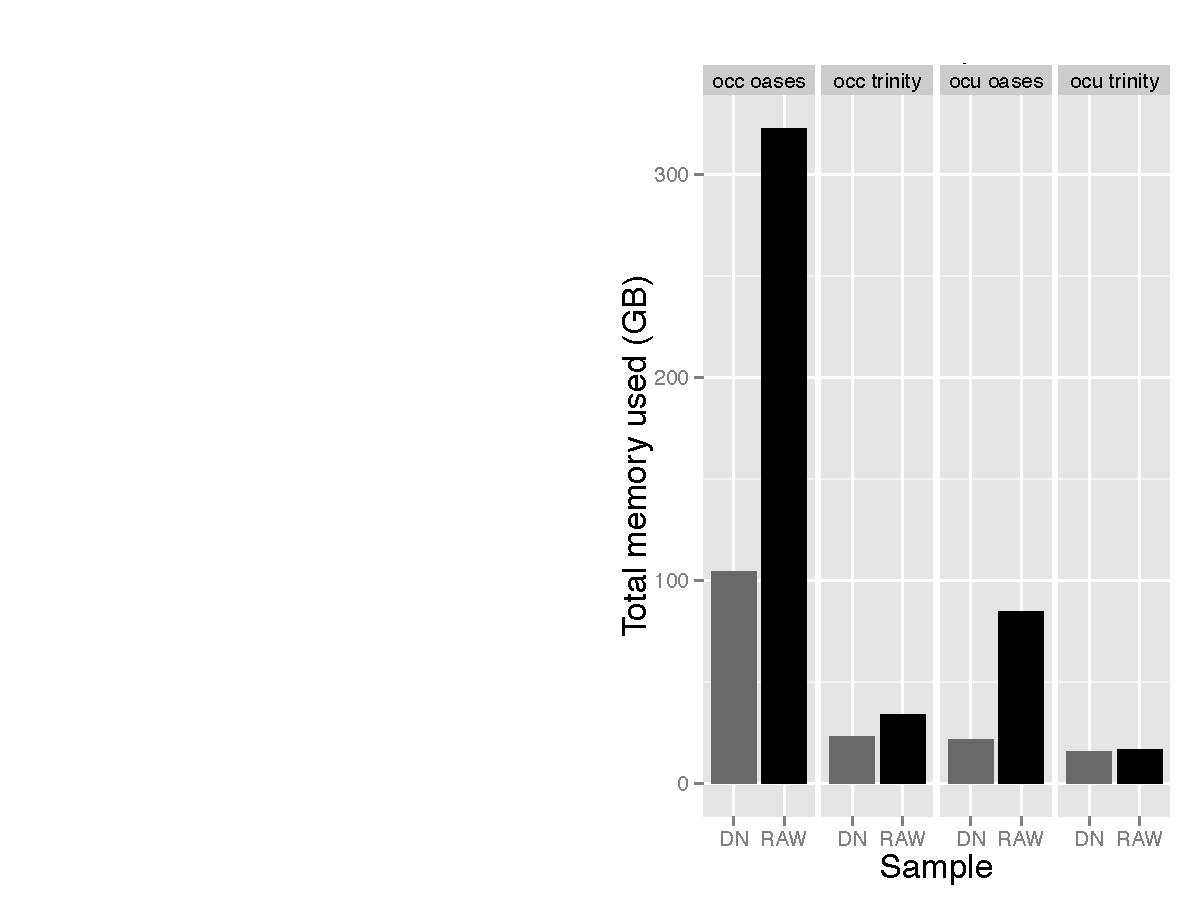
\includegraphics[width=0.45\textwidth]{manuscript/figure_1_memory.pdf}
	}
\caption{\textbf{Wall time and memory requirements for assemblies.} Wall time (a) in hours to complete the diginorm (DN) and raw read (RAW) assemblies for both species and assemblers. Oases assembled multiple k's, 21 $\leq$ k $\leq$ 35 opposed to Trinity that uses only a single k. This is one reason the assembly times differed. (b) Shows the memory used to assemble each of the transcriptomes. M. oculata (ocu) transcriptomes assemble in less time than M. occulta (occ) because they have fewer lanes of reads to assemble. In all cases diginorm required less time and memory to complete the assembly.}
\label{fig:time_and_memory.pdf}
\end{figure}
  
\subsection{Assembly statistics varied by preprocessing approach and assembler}
Oases run with the diginormed reads yielded fewer total transcripts than Oases run with the unnormalized reads. The \textit{M. oculata} diginorm assembly produced 300 fewer transcripts, and the \textit{M. occulta} diginorm assembly produced 227 fewer transcripts (Table~\ref{table:Table2.pdf}). Digital normalization had the opposite affect when using Trinity for assembly, increasing the total number of assembled transcripts by 7,840 for \textit{M. oculata} and 9,197 for \textit{M. occulta}.

\begin{table}[tbp]
\centering
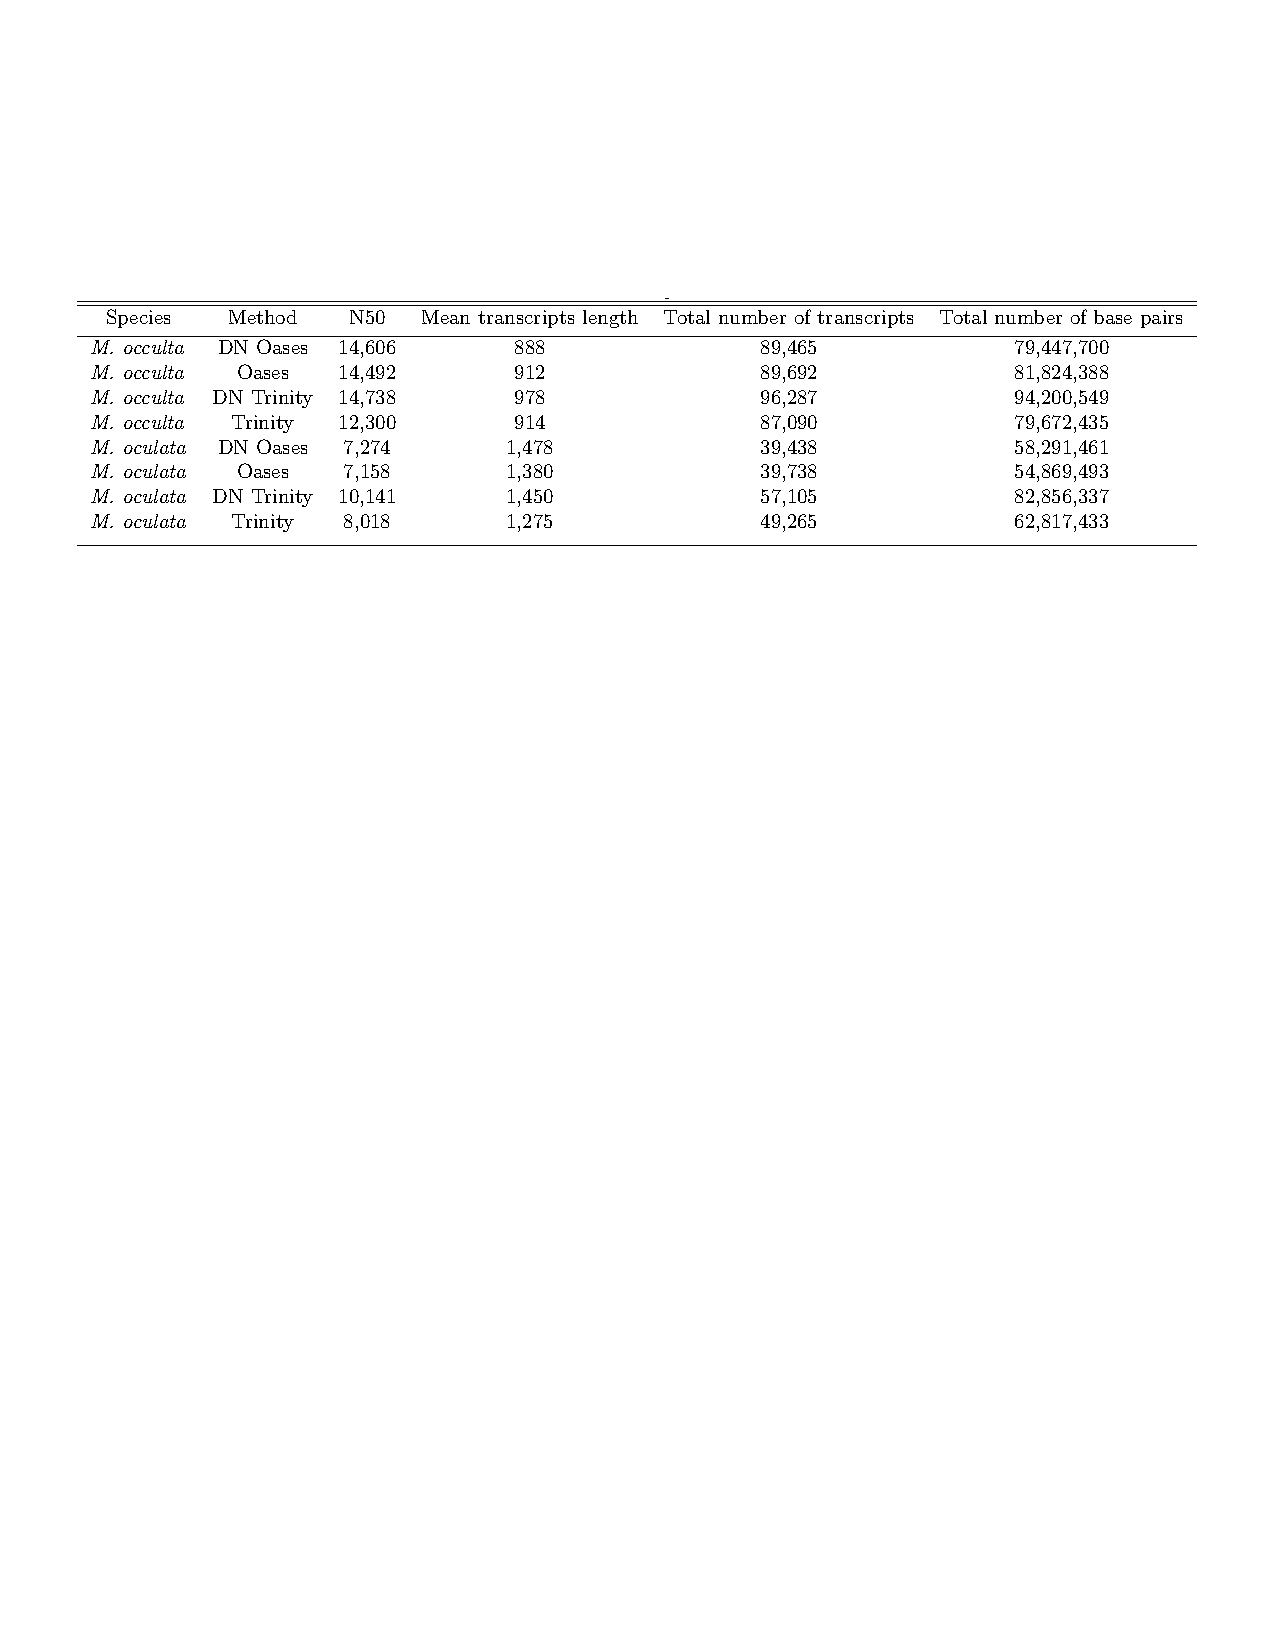
\includegraphics[width=\linewidth]{manuscript/Table2.pdf}
\caption{\textbf{Transcriptome metrics.} Several metrics used to assess the assembled transcriptomes. The N50, mean transcript length, total number of transcripts and total number of base pairs are listed for each transcriptomes.}
\label{table:Table2.pdf}
\end{table}
   
Trinity produces 6.8k (7.6\%) more transcripts than Oases for \textit{M. occulta} using the digitally normalized reads, and a 2.6k (2.9\%) decrease in the number of transcripts using the unnormalized reads. Trinity assembled more transcripts for both \textit{M. oculata} assemblies, a 17.6k (44.8\%) increase for diginorm and a 9.5k (24\%) increase for the raw reads. 

\subsection{Trinity assemblies include more low-abundance k-mers than Oases assemblies}
We next examined the k-mer spectrum of the assembled transcripts using k-mer abundances from the digitally normalized reads. The k-mer spectrum is an account of the information content of the reads and can be used to evaluate the ability of the assemblers to recover low-abundance transcripts \citep{pop_genome_2009}.  We first used digital normalization to reduce the reads to a median k-mer coverage of 20, so that the k-mer frequency spectrum peaked at a coverage of 20, and then plotted a cumulative abundance plot of those k-mers shared between the normalized reads and the assemblies. The results, displayed in Figure 2, show that Trinity recovers more low-abundance k-mers.  Also note that between assemblies done with the same assemblers, the k-mer distributions were very similar, suggesting that the k-mer spectrum is reflective of the underlying graph traversal algorithm used by the assembler. In addition the Trinity assemblies included more unique k-mers (Figure~\ref{fig:multiplicity})

\msulandscape{}
\begin{figure}[!H]
	\subfloat[\textit{M. occulta}\label{subfig-1:figure_2_Mocc_dist}]{%
	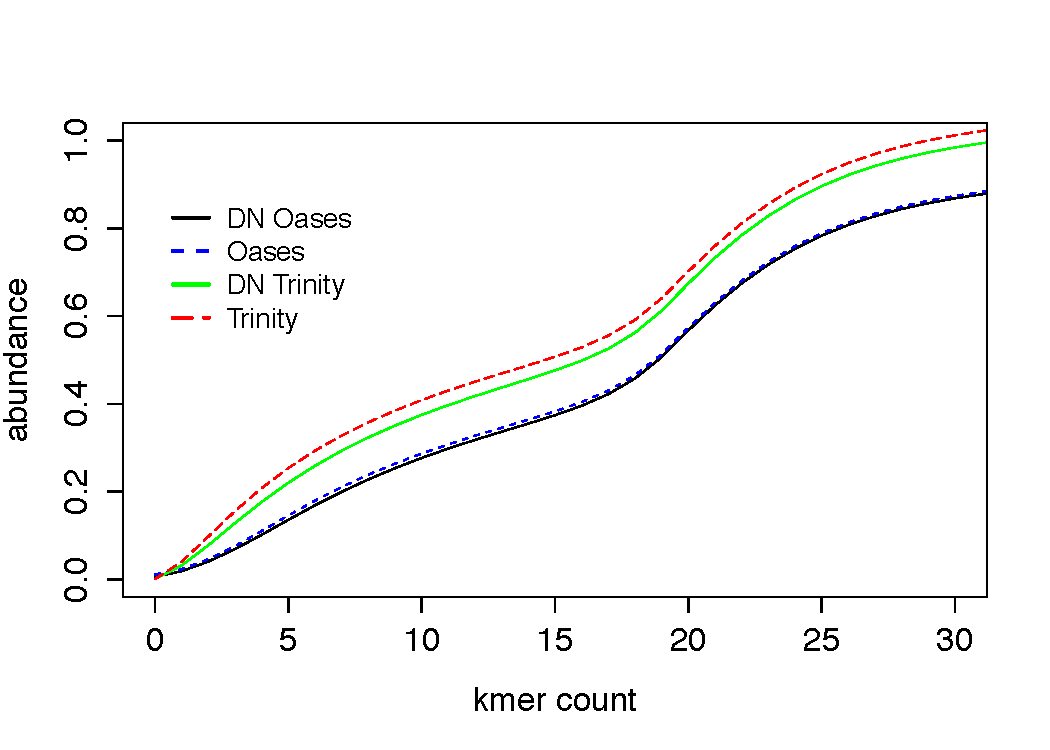
\includegraphics[width=0.65\textwidth]{manuscript/figure_2_Mocc_dist.pdf}
	}
	\hfill
	\subfloat[\textit{M. oculata}\label{subfig-2:figure_2_Mocu_dist}]{%
	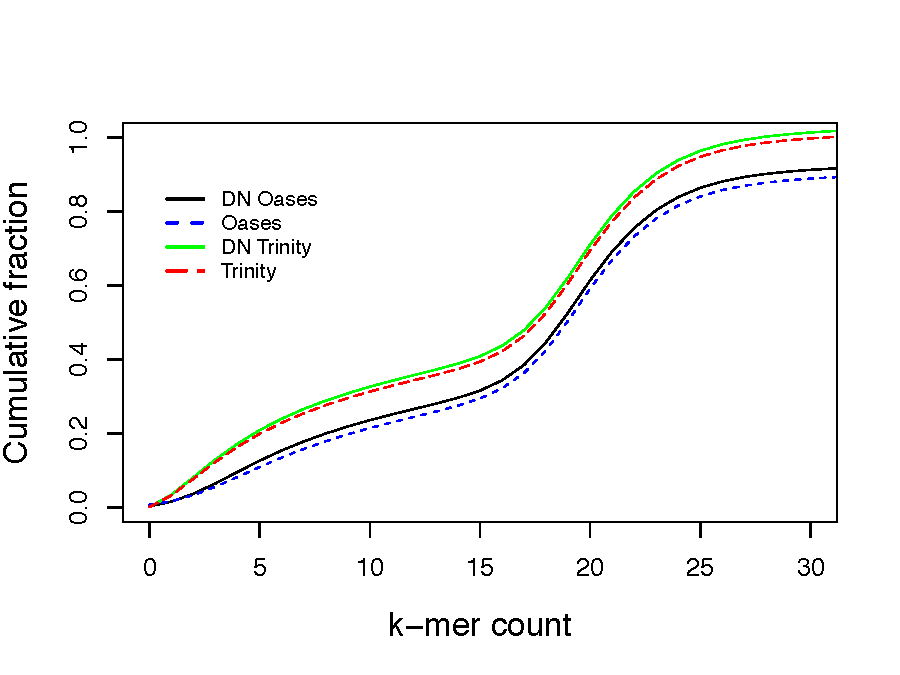
\includegraphics[width=0.65\textwidth]{manuscript/figure_2_Mocu_dist.pdf}
	}
	\caption{\textbf{K-mer distribution.} The k-mer distribution is shown for each assembler and assembly condition, diginorm (DN) and unnormalized reads. The k-mer distribution is the coverage of a given k-mer verses how many k-mers of that coverage is incorporated in the respective assemblies. Both Oases and Trinity assemblies are shown for (~\ref{subfig-1:figure_2_Mocc_dist}) \textit{M. occulta} k-mer distribution and  (~\ref{subfig-2:figure_2_Mocu_dist}) \textit{M. oculata} k-mer distributions. Trinity had a higher k-mer distribution for both species, reflective of the inclusion of more low abundance reads into the Trinity assemblies.}
	\label{fig:k-mer_spec}
\end{figure}
\endmsulandscape{}

\begin{table}[tbp]
\centering
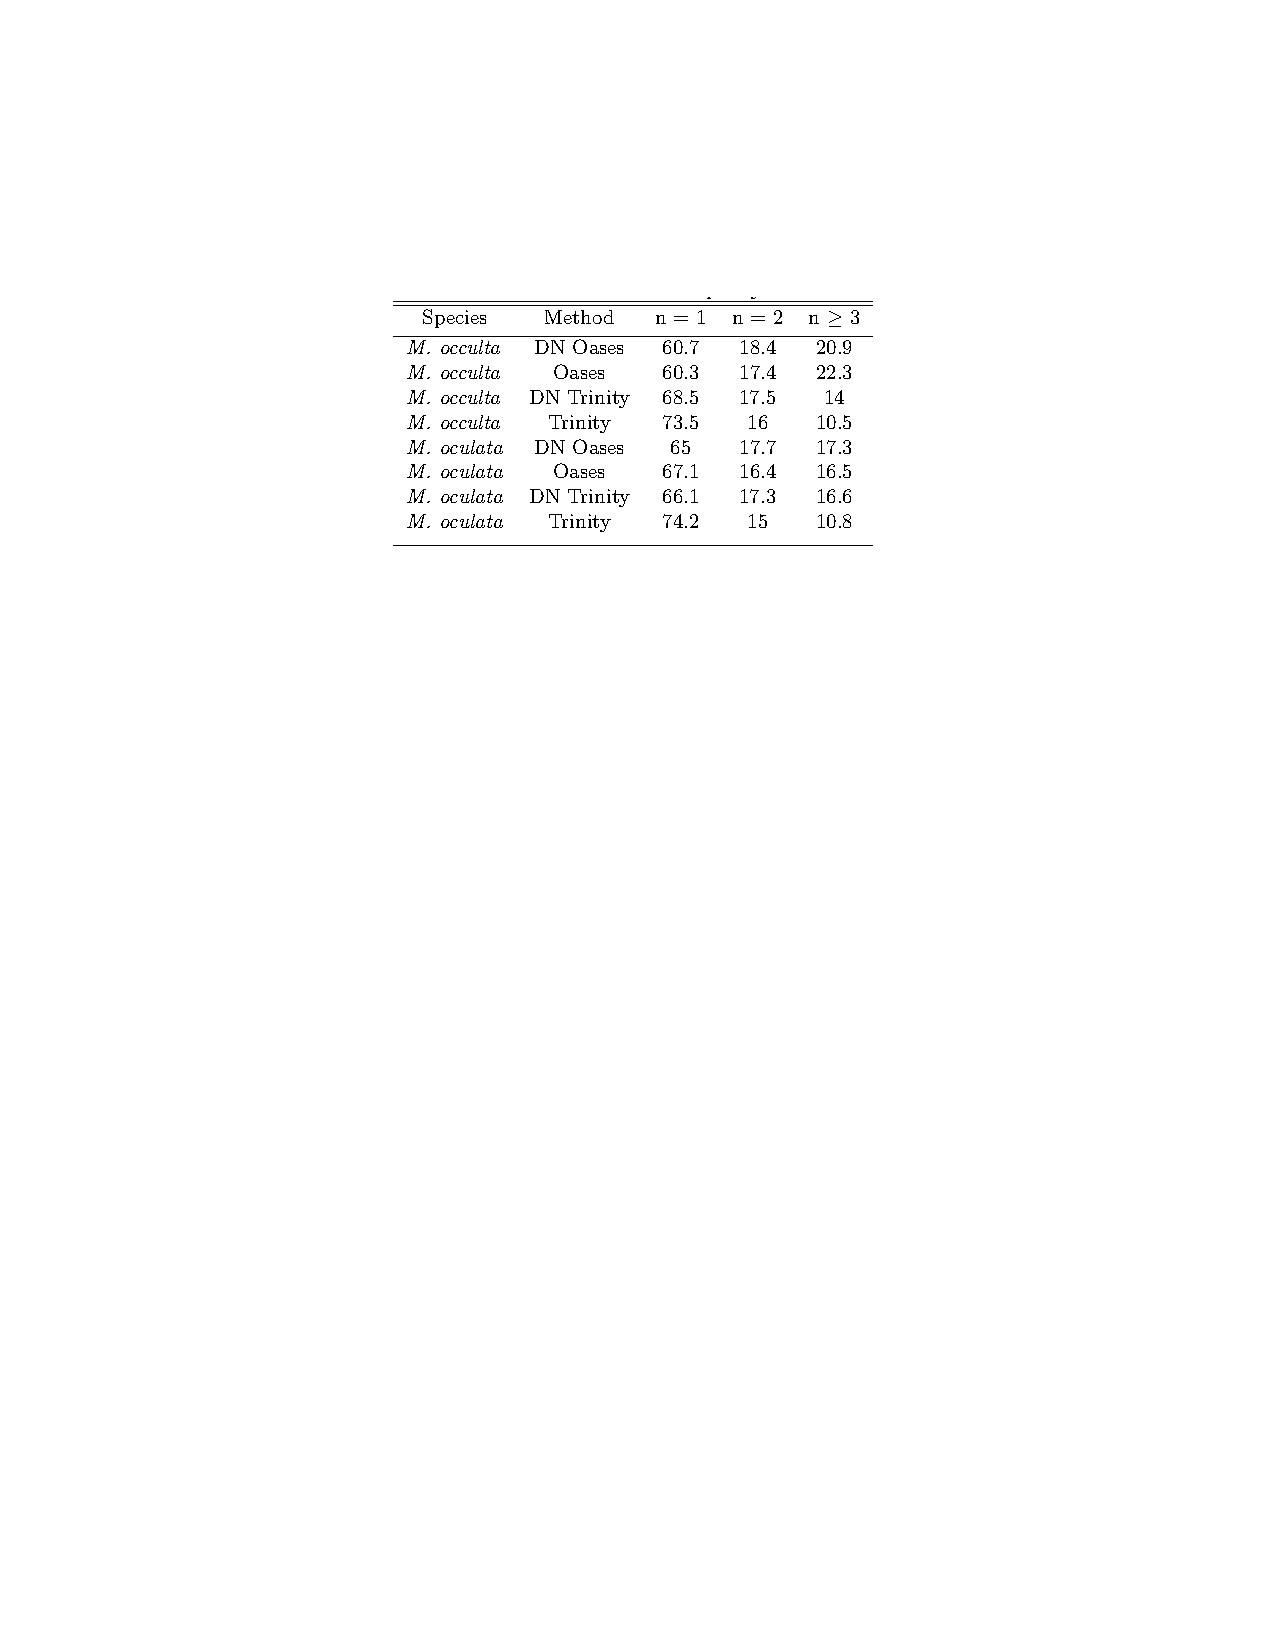
\includegraphics[scale=1]{manuscript/Table_3_multiplicity.pdf}
\caption{\textbf{Multiplicity.} The k-mer multiplicity shows uniqueness of each assembly. All k-mers with a multiplicity of one are unique. Trinity has a higher percentage of unique k-mers when comparing assemblers. The unnormalized Trinity had the highest number of unique k-mers overall.}
\label{fig:multiplicity}
\end{table}

\subsection{Read mapping shows high inclusion of reads in the assembled transcriptomes}
	We mapped the quality-filtered reads to the assembled transcriptomes to evaluate their inclusiveness. The F+3 stage of reads from \textit{M. occulta} had the lowest percentage of mapped reads, with the Oases unnormalized assembly mapping only 49\% of the reads, and the Trinity unnormalized assembly mapping 67\% (Figure~\ref{subfig-1:figure_3_mocc_mapping}). This was an isolated case: all other Oases assemblies contained at least 75\% of the reads for each time point and the Trinity assemblies contained at least 93\% of the reads for each time point. Trinity raw read assemblies tended to contain slightly more reads than the diginorm assemblies, while the opposite was true for Oases; however, in no case did the mapping of raw-reads assembly differ from the diginorm assemblies in more than 3\% of their read content.
\setcounter{subfigure}{0}

\msulandscape{}	
\begin{figure}[!H]
	\subfloat[\textit{M. occulta}\label{subfig-1:figure_3_mocc_mapping}]{%
	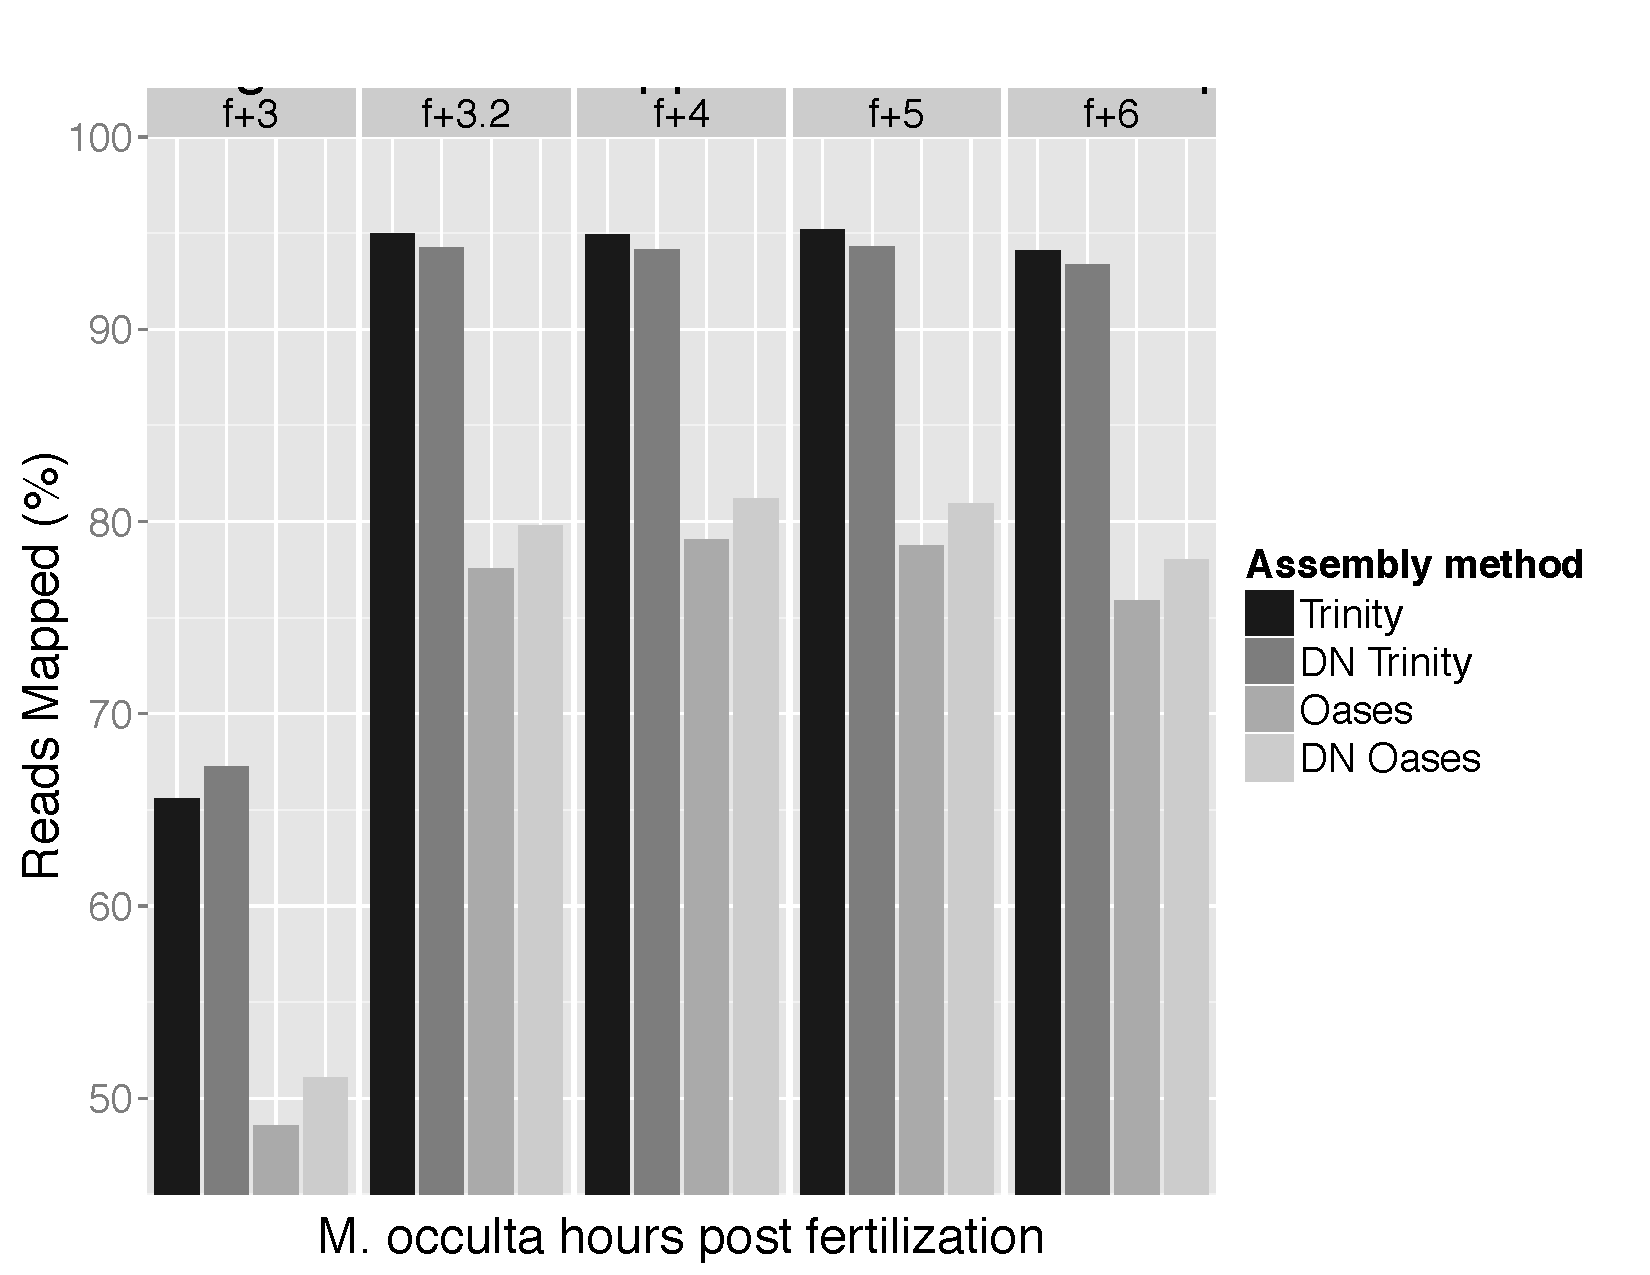
\includegraphics[width=0.65\textwidth]{manuscript/figure_3_mocc_mapping.pdf}
	}
	\hfill
	\subfloat[\textit{M. oculata}\label{subfig-2:figure_3_mocu_mapping}]{%
	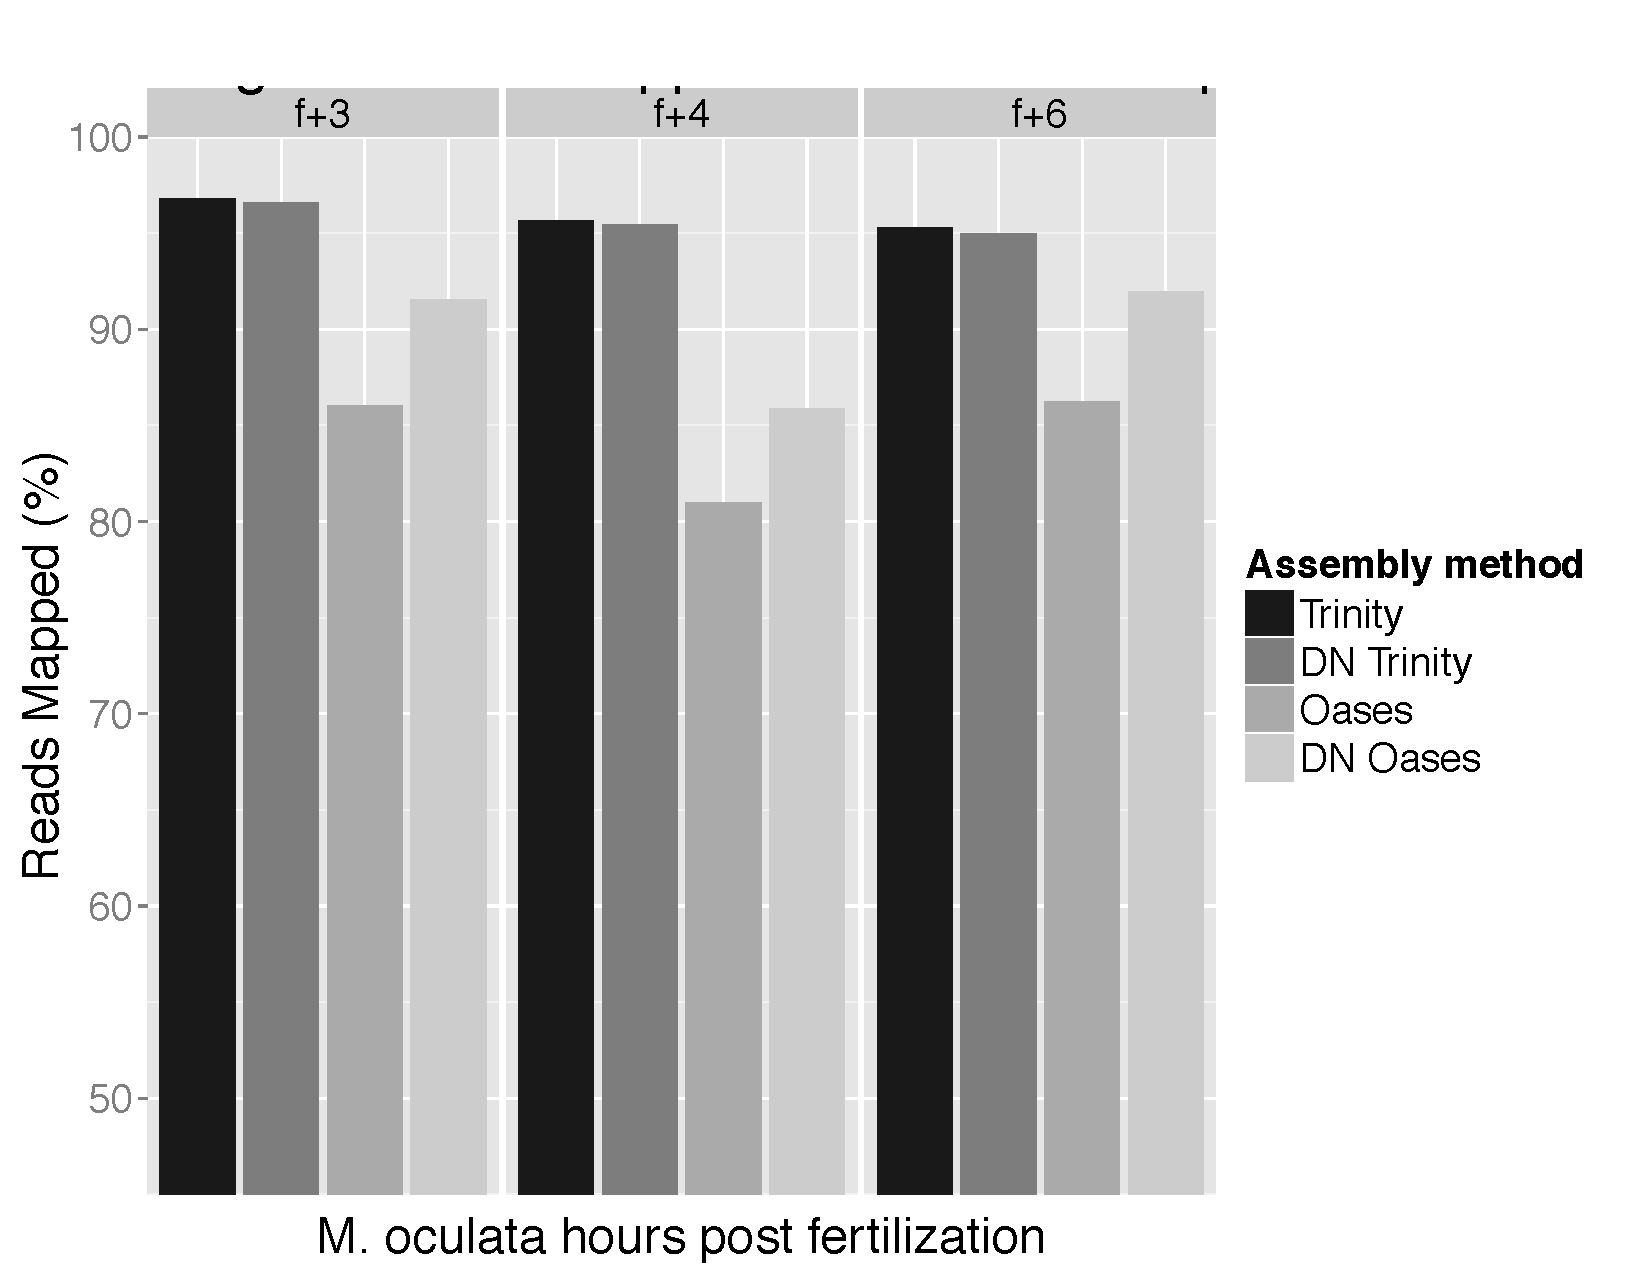
\includegraphics[width=0.65\textwidth]{manuscript/figure_3_mocu_mapping.pdf}
	}
	\caption{\textbf{Read mapping.} Unnormalized reads were mapped back to each of the assemblies to determine the inclusion of reads in the assembly. \textit{M. occulta} first round of gastrulation reads (f+3), showed the lowest mapping quality for all assemblies, with the lowest being raw Oases at 48.57\%. \textit{M. occulta} f+3 is the only case where mapping is less than 74\% and the only case where DN Trinity mapped more reads than raw Trinity. \textit{M. oculata} unnormalized Oases performed the worst, with the Trinity assembly having the best mappings. Trinity assemblies have more mapped reads than Oases for all conditions, with at least 93\% read mapping for both species. Raw Trinity typically mapped slightly more reads than DN, and the opposite occurs for Oases, with DN having more reads mapped to its assembly.  Note that the Y axis starts at 45\%.}
	\label{fig:read_mapping}
\end{figure}
\endmsulandscape{}

\subsection{All assemblies recovered transcripts with high accuracy but varied completeness}
mRNAseq assembly accuracy can be calculated based on known transcripts generated from longer reads or reference genomes \citep{vijay_challenges_2012,martin_next-generation_2011}. We use Molgulid nucleotide sequences from NCBI to measure accuracy, and we define accuracy as the average BLAST identity score for the best match for each gene recovered \citep{li_sequence_2009}. There are 178 sequences from within the Molgula clade in the NCBI database. With the exception of \textit{M. occulta} unnormalized Oases assembly, all assemblies have hits to at least 113 out of these Molgula sequences (Figure 4). The Trinity assemblies for both species have hits to all 178 sequences. Oases assemblies have hits for more sequences using digital normalized reads, two additional hits for \textit{M. oculata} and 40 additional hits for \textit{M. occulta}. \textit{M. oculata} assemblies hits have high average accuracy in the 90 and 99 percentile for Oases and Trinity, respectively. Completeness is the percentage of a gene, transcript or protein that is recovered. Within the \textit{M. oculata} assemblies, the unnormalized Oases assembly has the lowest average completeness at 36\%, the Trinity assemblies round out at 60\% and the digital normalized Oases assembly has the highest average completeness at 72\%.  (Note that many of the \textit{Molgula} sequences are genomic, which includes intronic regions, so we would expect this to lower the completeness scores.)
	
\msulandscape{}
\begin{figure}[!H]
	\begin{center}
	\subfloat[\textit{M. occulta}\label{subfig-1:figure_4_moccVsknownmolg}]{%
	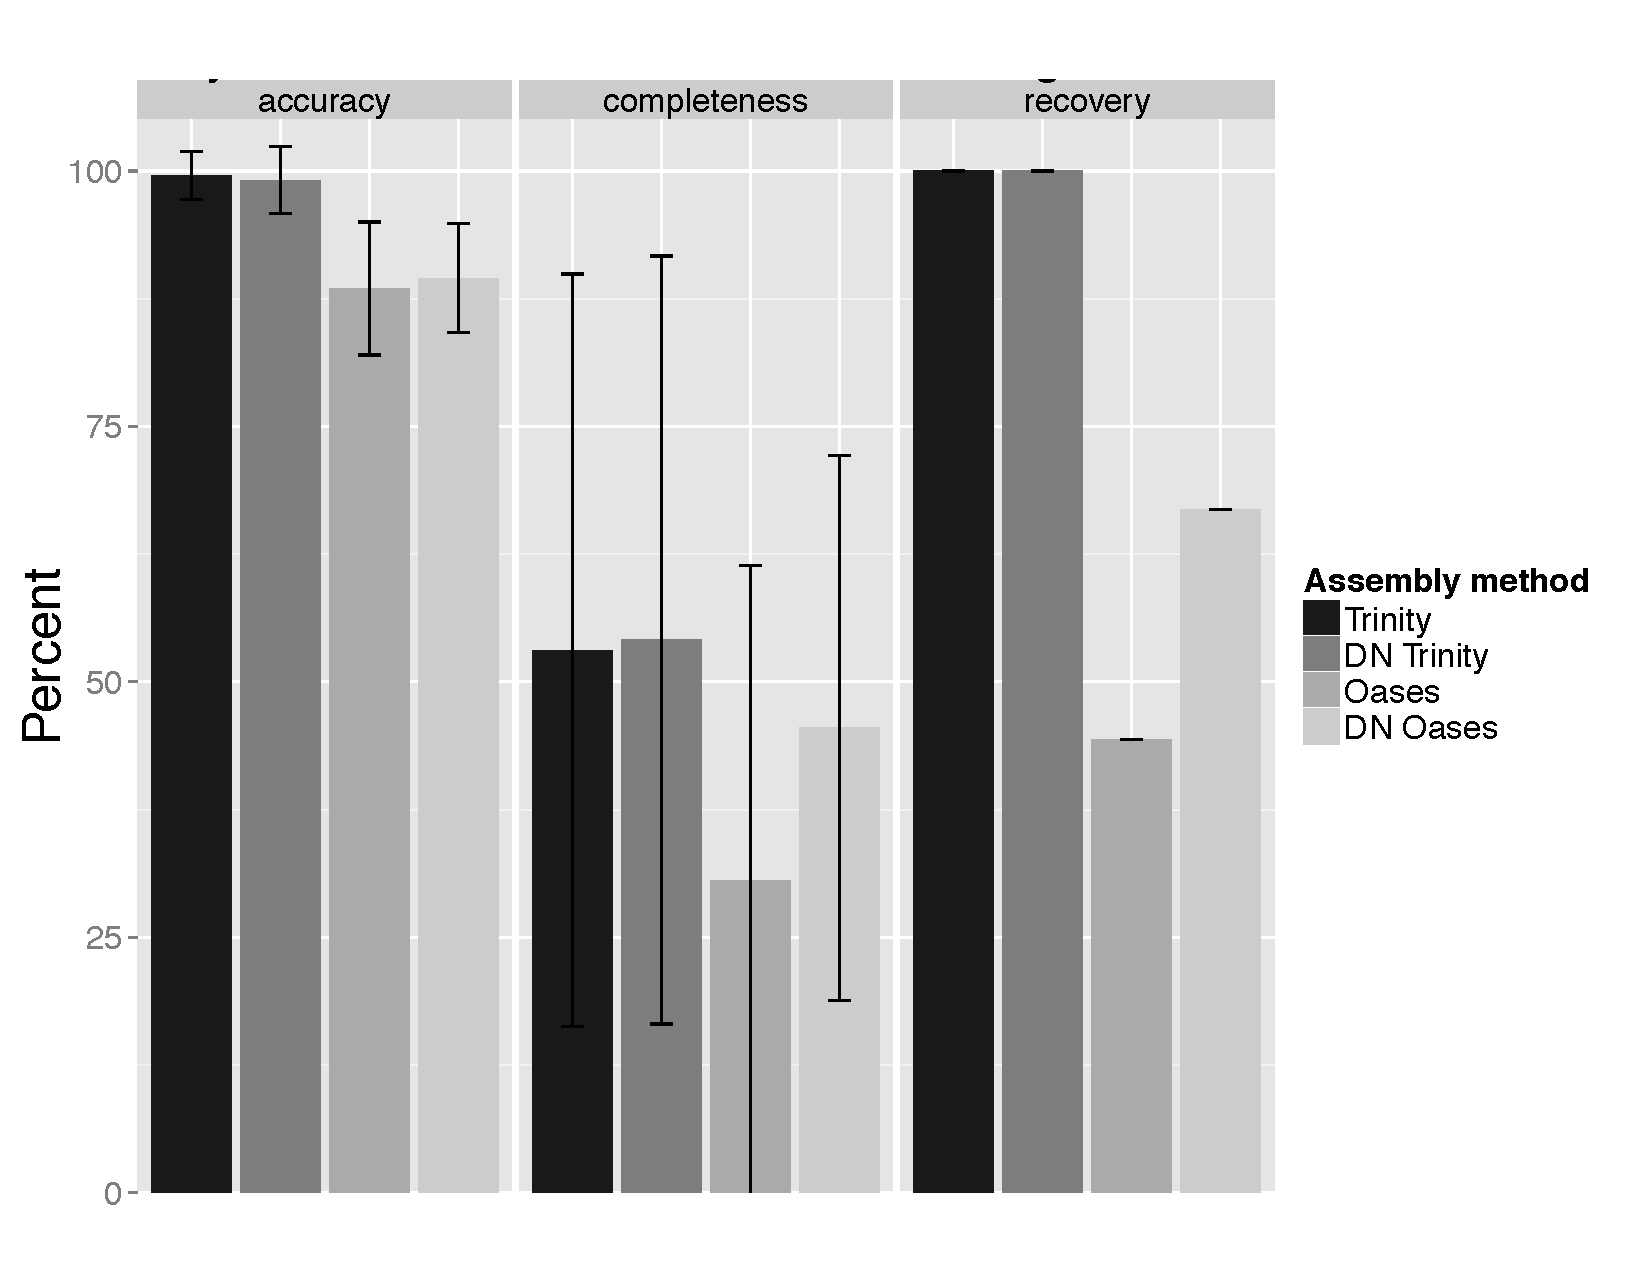
\includegraphics[width=0.67\textwidth]{manuscript/figure_4_moccVsknownmolg.pdf}
	}
	\hfill
	\subfloat[\textit{M. oculata}\label{subfig-2:figure_4_mocuVsknownmolg}]{%
	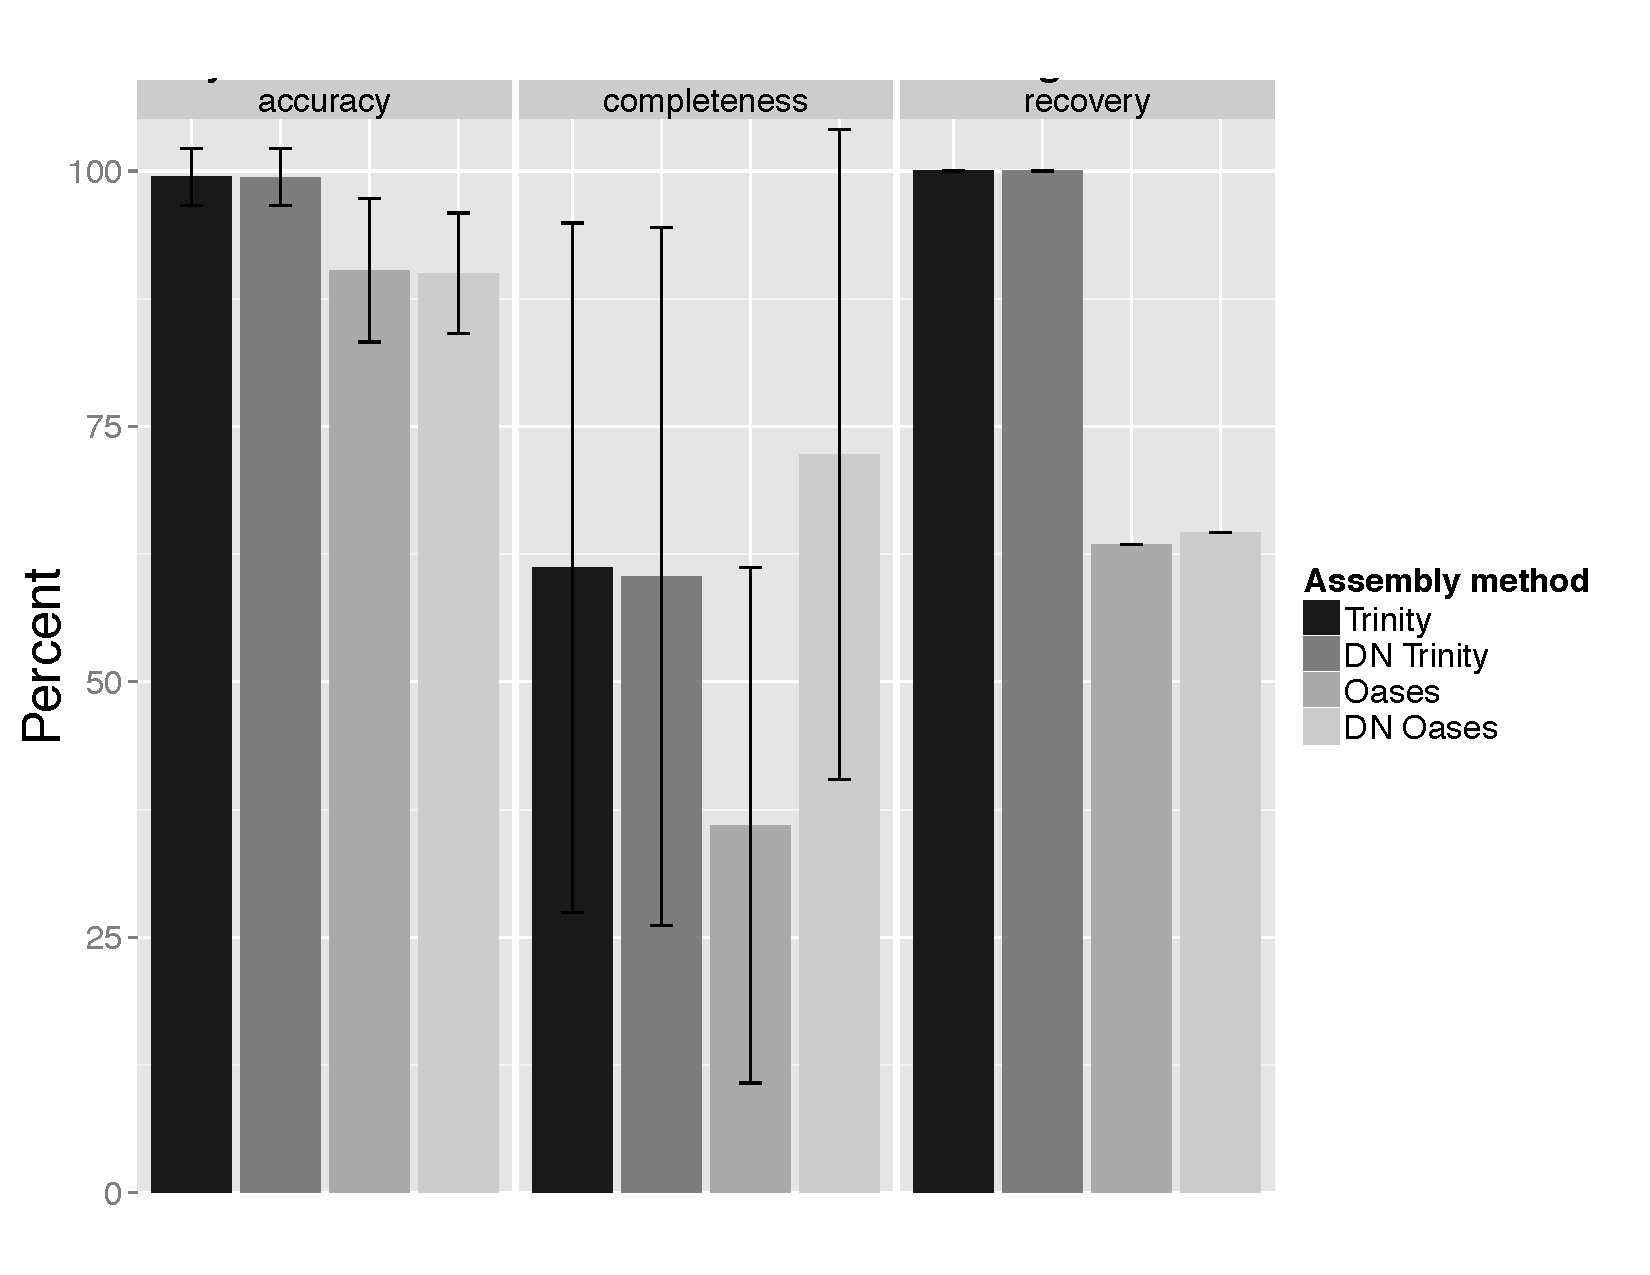
\includegraphics[width=0.67\textwidth]{manuscript/figure_4_mocuVsknownmolg.pdf}
	}
	\caption{\textbf{Accuracy, completeness and recovery rate against known Molgula sequences.} The NCBI has 178 Molgula sequence in its database. Transcripts were searched against these sequences using BLASTN with a cut-off of 1e-12. Trinity assemblies performed the best, recovering all known sequences. The \textit{M. occulta} unnormalized assembly performed the worst, only recovering 79 (44\%) of the transcripts. \textit{M. occulta} tended to recover fewer of the known transcripts as well.}
	\label{fig:known_molg}
	\end{center}
\end{figure}
\endmsulandscape{}
     
Of these 178 nucleotide sequences, 8 of them are \textit{M. occulta} sequences and 15 of them are \textit{M. oculata} sequences. All \textit{M. occulta} assemblies recovered all 8 of the NCBI \textit{M. occulta} sequences with a 94\% or greater accuracy. \textit{M. oculata} assemblies recovered \textit{M. oculata} transcripts at a 93\% accuracy as well. \textit{M. occulta} assemblies produced the lowest completeness of the two species, 41\% and 43\% for unnormalized Oases and diginorm Oases respectively, and 75\% for both Trinity assemblies. \textit{M. oculata} assemblies produced more complete transcripts 66, 75, 86, and 83 percent for unnormalized Oases, Diginorm Oases, unnormalized Trinity and Diginorm Trinity respectively.


\subsection{Both unnormalized and normalized assemblies recovered many of the same transcripts}
We evaluated the two diginorm and unnormalized assemblies against one another to test whether either method missed significant portions of the transcriptome assembled by the other. We used BLAT to compare unnormalized and diginorm assemblies in both directions. In \textit{M. occulta}, both methods recovered at least 93\% of the transcripts, with Trinity diginorm recovering \mytilde99\% of Trinity's unnormalized assembly. \textit{M. oculata} assemblies showed high overlap as well, all recovering greater than 98\% of each other with the exception of diginorm Oases recovering 94\% of unnormalized Oases assembly.

\subsection{Homology search against the \textit{Ciona} proteome shows similar recovery of ascidian genes across assemblies}
We used \textit{Ciona intestinalis} to evaluate the completeness of our transcriptomes. \textit{C. intestinalis} has an assembled genome that is well annotated and is the closest available genome to the Molgulids. \textit{C. intestinalis} has a genome of ~160 Mb and contains \mytilde16,000 genes \citep{satoh_surfing_2005}. A total of 13, 835 (86\%) of the \textit{C. intestinalis} proteins found in NCBI had hits in the \textit{M. occulta} transcriptomes (Figure 5), with 2,288 genes (14\%) having no hits due presumably to either lack of expression, high divergence, or loss \textit{M. occulta}. When comparing transcripts excluded by either diginorm or unnormalized reads for all assemblies, the unnormalized read assemblies produced an additional 0.04\% hits to \textit{C. intestinalis} and there was additional 0.03\% for the diginorm assemblies. There was little difference between the assemblies when compared to \textit{C. intestinalis}, with 99\% of the \textit{C. intestinalis} genes being found in all \textit{M. occulta} assemblies (Figure 4a). Eighty-six percent of the \textit{C. intestinalis} proteins had matches in the \textit{M. occulta} and \textit{M. oculata} assemblies with less than 1\% difference in presence between the several assemblies (Figure 4b).


\msulandscape{}
\begin{figure}[!H]
	\subfloat[\textit{M. occulta}\label{subfig-1:figure_5_mocc_blast_overlap}]{%
	\includegraphics[width=0.65\textwidth]{manuscript/figure_5_mocc_blast_overlap.pdf}
	}
	\hfill
	\subfloat[\textit{M. oculata}\label{subfig-2:figure_5_mocu_blast_overlap}]{%
	\includegraphics[width=0.65\textwidth]{manuscript/figure_5_mocu_blast_overlap.pdf}
	}
	\caption{\textbf{Gene recovery, raw reads versus normalized.} Gene similarity with \textit{C. intestinalis} via BLAST for \textit{M. occulta} (left) and \textit{M. oculata} (right). Each oval represent the total number of putative homologous sequences recovered. In both species the Trinity assembler assembled more homologous sequences. There was almost complete overlap in homology for both assemblers and both assembly conditions.}
	\label{fig:overlap}
\end{figure}
\endmsulandscape{}


We next examined the difference between the unnormalized and digitally normalized assemblies. Transcripts in the unnormalized assembly with BLAST hits to \textit{C. intestinalis} but without hits in diginorm assemblies were extracted, and searched using BLASTN against the diginorm assemblies; we found fragmented versions of these transcripts, suggesting that they were partially assembled.  We then mapped the diginorm reads to the extracted unnormalized transcripts and found that some portions of the transcripts were not covered by the normalized reads. This demonstrates that these transcripts were lost due to a loss of information from the diginorm process.  However, the overall loss was minimal and complemented by an increase in the recovery of other conserved transcripts; this is clearly a direction for further study.
\subsection{CEGMA analysis shows high recovery of genes}
CEGMA uses a list of highly conserved eukaryotic proteins to evaluate genome and transcriptome completeness \citep{parra_cegma:_2007}. We used CEGMA to analyze the number of protein families that are present in each assembly. The default CEGMA parameters were used for analysis. CEGMA reports recovery as ``complete'' or ``partial'', where a match is marked as ``complete'' if 70\% or more of the amino acid sequence is recovered. More than 90\% of the CEGMA genes were recovered completely in each of the transcriptome assemblies, while greater than 98\% of the CEGMA genes were recovered at least partially. 

\section{Discussion}

\subsection{Transcriptome assembly accurately recovers known transcripts and many genes}

% @CTB - removed. Diginorm increased the recovery rate for the known Molgula nucleotides for the Oases assemblies. Diginorm did not have much of an effect on \textit{M. oculata}, however, \textit{M. occulta} which has 10s of millions more reads, had a much more noticeable effect, with a 51\% increase in recovered sequences. Diginorm also had a positive effect on the completeness of transcripts when assembling with Oases. Trinity performed better than Oases whether the reads are digitally normalized or unnormalized. Completeness was not over 60\% for any of the assemblies, but this is explained by the fact that most of the nucleotide sequences were not mRNA so our transcripts would not align to the intronic regions. This confirms that all assembly techniques yielded good transcriptomes when applied to both data sets.

All of the transcriptome assemblies yielded homologs for an almost identical subset of the \textit{Ciona intestinalis} proteome.  While the evolutionary distance between the Molgulids and \textit{C. intestinalis} may be large -- the Molgulids are stolidobranch ascidians and are believed to be very divergent from \textit{C. intestinalis}, which is a phlebobranch ascidian \citep{huber_evolution_2000, stach_phylogeny_2002}\textemdash approximately 84\% of \textit{Ciona} proteins were found in all assemblies via BLAST, and more than 44\% of \textit{Ciona} proteins had putative orthologs in each of our assemblies via reciprocal best hit.  Since both transcriptomes are from a limited set of embryonic tissues that do not express all genes, these are surprisingly high numbers!  We infer that we have recovered almost all embryonic genes and the majority of genes present in the Molgula genomes.

Read mapping and CEGMA analyses further confirm that the transcriptome assemblies are of high quality and inclusiveness.  The assemblies represent 75\% or more of the reads from all but one time point, contain complete matches to 90\% or more of the conserved eukaryotic gene families in CEGMA, and contain partial matches to 98\% or more of the CEGMA families.   It is important to note that the CEGMA results are almost certainly biased upwards by the nature of the CEGMA families, which represent many more metabolic and cellular function genes than e.g. animal-specific transcription factors; thus the CEGMA numbers do not directly demonstrate the inclusiveness of the transcriptome families, as they would for a genome assembly \citep{parra_cegma:_2007}.

\subsection{Digital normalization eases assembly without strongly affecting assembly content}

One of our goals in this study was explore the impact of digital normalization on the biological interpretation of transcriptome assemblies; while previous studies have shown that digital normalization can make assembly faster and less memory intensive, gene recovery has been less well studied \citep{haas_novo_2013, brown_reference-free_2012}.  Here we confirm the computational results: diginorm dramatically reduces the computational cost of Oases assemblies, and also decreases the time and memory requirements for Trinity assemblies.

While digital normalization does alter the number of transcripts significantly, it does not strongly affect either read inclusion or the conserved gene content of the assemblies. Read inclusion by mapping never decreased more than 3\% after digital normalization, and in many cases increased. The conserved gene content, measured by a proteome comparison, showed that we recover essentially the same set of proteins with all four treatments on both transcriptomes.  

Combined, these results suggest that the varying number of transcripts largely reflect differences in the splice variants reported by different assemblers under different conditions. These results also strongly support the idea that preprocessing with digital normalization does not strongly affect assembly content.  We note, however, that the few transcripts not recovered in assemblies of the digitally normalized reads were probably not recovered because the underlying reads were eliminated during digital normalization.  This is an area where digital normalization can be improved.

Only a small number (well below 1\%) of different homology matches were reported between the various assemblies.  Because of this we decided not to merge or otherwise combine the different assemblies: the likely benefits were outweighed by the risk of introducing chimeric transcripts or combining isoforms.

We also note that the variation in number of assembled transcripts due to read preprocessing and choice of assembler despite the similar gene content suggests that traditional genome assembly metrics such as number of transcripts, total bp assembled, and N50 are not useful for transcriptome evaluation as previously suggested \citep{oneil_assessing_2013}.  For example, the same exon may be included in multiple splice variants, inflating the total bp assembled; some assemblers may choose to report more isoforms than others even with the same read support; and N50 makes little sense for transcriptomes.
 
\subsection{Trinity assemblies are more sensitive to low-abundance k-mers but contain no new conserved genes}
The difference in transcript numbers between Trinity and Oases assemblies is stark: for the same data set, with the same treatment, Trinity always produces thousands more transcripts than Oases.  Moreover, many more reads can be mapped to the Trinity assemblies \textemdash an additional 10\% or more, for every stage.  Despite this greater inclusion of reads, we see no substantial gain in either CEGMA matches or \textit{Ciona} proteome matches for the Trinity assemblies.

This conundrum can be resolved by examining the k-mer spectra, which show that the Trinity assemblies include many more low-abundance k-mers from the read data set.  This demonstrates that Trinity is more sensitive to low-abundance sequences, and may include more isoforms in its assemblies\textemdash by design, Trinity attempts to be more sensitive to isoforms than Oases, and focuses particularly on low-coverage isoforms \citep{vijay_challenges_2012, grabherr_full-length_2011, van_belleghem_novo_2012}. Those transcripts were indeed the results of Trinity assembling low coverage reads, having an average coverage of 5x compared to 75x.
 
\section{Conclusions}
We show that transcriptome assembly on two closely related species of Molgulid ascidians produced accurate and high-quality transcriptomes, as determined by several different metrics.  Importantly, four different assembly protocols produced transcriptomes that contained nearly identical complements of homologs to the nearest model organism, \textit{Ciona intestinalis}.  While variations in isoform content were observed, these variations had little apparent impact on sensitivity of homologous gene recovery. We provide detailed assembly protocols that should enable others to easily achieve \textit{de novo} transcriptome assemblies.

\section{Acknowledgments}

EKL and this research were supported by the National Science
Foundation under Cooperative Agreement No. DBI-0939454 (BEACON). Any
opinions, findings, and conclusions or recommendations expressed in
this material are those of the authors and do not necessarily reflect
the views of the National Science Foundation.  CTB was supported in
part by Agriculture and Food Research Initiative Competitive Grant
no. 2010-65205-20361 from the United States Department of Agriculture,
National Institute of Food and Agriculture.


\chapter[title]{Genome assembly and characterization\footnote{Portions of this section were published in Stolfi et al., \cite{stolfi_guidelines_2014}.}}
\section{Introduction}
Ascidians are marine invertebrates that spend their adult life filter feeding through an incurrent siphon and an outcurrent siphon. Ascidians are evolutionarily interesting because of the phylogenetic position -- they are tunicates, the sister group to vertebrates and cephalochordates, with whom they form the chordate phylum. Although ascidians share little morphological resemblance to vertebrates in their adult stage, they do share several features in their larval stage: a notochord, dorsal hollow neural tube, and gill slits during development \cite{wada_details_1994,cameron_evolution_2000}. 

The development of ascidians is well documented, and the cell lineage from fertilization to gastrulation has been described thoroughly in \textit{Ciona intestinalis} \cite{nishida_cell_1983,nishida_cell_1985,nishida_cell_1987}. Studies of other ascidian species have shown that the majority of the phyla members have an invariant cell lineage and typical development \cite{berrill_studies_1931}. However, a few solitary ascidians have deviated from the typical developmental program and undergone tail-loss \cite{swalla_interspecific_1990, tsagkogeorga_updated_2009}. \textit{M. occulta} and \textit{M. oculata} are two species that are found in the shallow waters for Roscoff, France that closely resemble each other-- in their adult stage, they differ only by a white pigment spot found between the siphons of \textit{M. oculata} (Figure~\ref{fig:adults}). These two \textit{Molgula} species, however, have different methods of development\textemdash \textit{M. oculata} develops as a typical tadpole larvae and \textit{M. occulta} develops without a tail. The underlying molecular reasons for divergence are unknown.

Many ascidian genes have been studied across a number of ascidians, showing that gene function tends to be orthologous within the phyla \cite{satoh_ascidian_2003}. Although genes tend to be expressed in homologous patterns and tissues, the presence of genes are not the same across species. There are a number of cases where a gene that has been shown to be necessary for a phenotype in one species is completely absent in other ascidian species with the same phenotype \cite{lemaire_ascidians_2008}. Ascidian species are far more divergent than they appear phenotypically. It has been shown that in ascidians with the same phenotype and gene expression, regulatory modules are not necessarily the same \cite{hudson_divergent_2011,kugler_evolutionary_2011,stolfi_divergent_2014}. This is often attributed to the conservation of gene regulatory networks (GRNs) and the flexibility of TF binding site distribution in a given enhancer, which contribute to conservation of enhancer function \cite{hare_careful_2008}. This regulatory turnover is termed ``developmental system/systems drift'' (DSD) \cite{true_developmental_2001}. This term broadly applies to the divergence in the molecular or morphogenetic basis for the development of identical homologous characters. 

Tunicates have even deviated from \textit{hox} patterning and function \cite{ikuta_limited_2010}, and here genomics has shed some light on the area. Ascidians are broadcast spawners, which leads to them being highly polymorphic and having rapid rates of evolution \cite{dehal_draft_2002}. This drives rapid divergence in genomes outside of coding regions, as well as change of gene function when compared to other chordates \cite{lemaire_ascidians_2008}. %We will demonstrate this divergence using two closely related species \textit{M. occulta} and \textit{M. oculata}, and the more divergent \textit{M. occidentalis}. 
Through whole genome sequencing and assembly of two closely related species \textit{M. occulta} and \textit{M. oculata}, and the more divergent \textit{M. occidentalis}, we have %given us a better picture of what is going on evolutionarily for both close and divergent species, and allows us to characterize gene networks, identify regulatory elements and gain better understanding of the mechanisms driving conserved development in ascidians.
demonstrated that \textit{M. occidentalis}, \textit{M. occulta}, and \textit{M. oculata} all have different \textit{hox} configurations, and while having invariant development, the cis-regulatory elements behind the development have diverged between \textit{Ciona} and \textit{Molgula}.

\begin{figure}[tbp]
\centering
\includegraphics[scale=0.5]{figures/adults.pdf}
\caption{\textbf{Adult ascidians.} \textit{M. occulta} (A) and \textit{M. oculata} (B) are nearly identical in their adult stage with the white pigment spot (red arrow). Their tunic is covered in sand, since they are found on the sandy sea bottoms. Under their sand covered tunic, the two species differ by the color of their eggs\textemdash purple in \textit{M. oculata}, pictured, and an orange-yellowish color in \textit{M. occulta}\textemdash which are found just above the kidney complex (C). \textit{C. intestinalis} (D) is the best studied ascidian and has a well-assembled and annotated genome \cite{dehal_draft_2002,satou_improved_2008}.}
\label{fig:adults}
\end{figure}

\section{Materials and methods}

\subsection{Genomic DNA library preparation and sequencing}
Genomic DNA was phenol/chloroform extracted from dissected gonads of \textit{Molgula occulta} (Kupffer) and \textit{Molgula oculata} (Forbes) adults from Roscoff, France, and a \textit{Molgula occidentalis} (Traustedt) adult from Panacea, Florida, USA (Gulf Specimen Marine Lab). Genomic DNA was sheared using an M220 Focused-ultrasonicator (Covaris, Woburn, MA). Sequencing libraries were prepared using KAPA HiFi Library Preparation Kit (KAPA Biosystems, Wilmington, MA) indexed with DNA barcoded adapters (BioO, Austin, TX). Size selection was performed using Agencourt (Beckman-Coulter, Brea, CA) AMPure XP purification beads (300-400 bp fragments), or Sage Science (Beverly, MA) Pippin Prep (650-750 bp and 875-975 bp fragments). For \textit{M. occulta} and \textit{M. occidentalis} libraries, 6 PCR cycles were used. For \textit{M. oculata} libraries, 8 cycles were used for the 300-400 bp library, and 10 cycles were used for the 650-750 and 875-975 bp libraries. Libraries of different species but same insert size ranges were multiplexed for sequencing in three 2x100 PE lanes on a HiSeq 2000 sequencing system (Illumina, San Diego, CA) at the Genomics Sequencing Core Facility, Center for Genomics and Systems Biology at New York University (New York, NY). Thus, each lane was dedicated to a mix of species, specifically barcoded libraries of a given insert size range. Raw sequencing reads were deposited as a BioProject at NCBI under the ID\# PRJNA253689.
\subsection{Genome sequence assembly}
All genomes were assembled on Michigan State University High Performance Computing Cluster (\url{http://contact.icer.msu.edu}). Prior to assembly, read quality was examined using FastQC v0.10.1. Reads were then quality trimmed on both the 5' and 3' end using seqtk trimfq (\url{https://github.com/lh3/seqtk}) which uses the Phred algorithm to determine the quality of a given base pair. Seqtk trimfq only trims bases, so no reads were discarded. Each library per species was then abundance filtered using 3-pass digital normalization to remove repetitive and erroneous reads \cite{brown_reference-free_2012,schwarz_genome_2013,howe_tackling_2014}. Genome assembly was done using velvet v1.2.08 \cite{zerbino_velvet:_2008} with k-mer overlap length (`k') ranging from 19 to 69 and scaffolding was done by Velvet, by default. Velvet does not produce separate files for contigs and scaffolds; because Velvet scaffolded conservatively, contigs dominated the assemblies so we refer to both contigs and scaffolds as contigs. CEGMA scores were then computed to evaluate genome completeness \cite{parra_cegma:_2007}. The latest versions of three species' genome assemblies have been deposited on the ANISEED (Ascidian Network for In Situ Expression and Embryological Data) database for browsing and BLAST searching at http://www.aniseed.cnrs.fr/ \cite{tassy_aniseed_2010}. Scripts for genome assembly and CEGMA analysis can be found in the following github repository: \url{https://github.com/ged-lab/2014-molgula-genome-assemblies}
\subsection{Gene identification and alignments}
Thirty-nine hox genes were identified in human and downloaded from the NCBI database. These sequences were then BLASTed against each of the three assembled \textit{Molgula} genomes. The alignments were then extracted and BLASTed against the NCBI non-redundant database. \textit{Molgula} aligning sequences were extracted, annotated and placed in the following files, mocc\_hox\_aa.fa, mocu\_hox\_aa.fa, and moxi\_hox\_aa.fa, which are located at \url{https://github.com/ged-lab/2014-elijahlowe-thesis} in the directory data/. \textit{Hox1-13} sequences for human, fruit fly, and Amphioxus were download from `Homeobox Database' (http://homeodb.zoo.ox.ac.uk/). These sequences were then joined in a multifasta file with the identified Molgula \textit{hox} genes and used to produce a phylogenetic trees using MAFFT version 7 online rough tree program at \url{http://mafft.cbrc.jp/alignment/server/clustering.html} \cite{katoh_parttree:_2007,katoh_mafft_2013}.  Additional alignments between the three species were conducted using mVista \cite{mayor_vista_2000,frazer_vista:_2004,visel_vista_2007} with \textit{M. oculata} as the anchoring sequence because it shows the most similarity between the three \textit{Molgula} species. The LAGAN alignment algorithm was used with translated anchoring to improve alignment because of evolutionary distances\cite{brudno_lagan_2003}.    

\section{Results}
\subsection{Genome assemblies assessment}
Genomes of three Molgula species (\textit{M. occidentalis}, \textit{M. oculata}, and \textit{M. occulta}) were sequenced using next-generation sequencing technology and assembled. A common metric for judging the quality of a genome assembly is the contig N50 length, which is determined such that 50\% of the assembly is contained in contigs of this length or greater. We used the contig N50 length to select the best assembly for each species given the varying `k' parameter (length of k-mer overlap). A `k' of 39 yields the best assembly for both \textit{M. occidentalis} and \textit{M. occulta}. The best `k' for \textit{M. oculata} was 61. \textit{M. occidentalis}, \textit{M. occulta}, and \textit{M. oculata} N50 lengths were approximately 26.3 kb, 13 kb, and 34 kb, respectively (Table~\ref{table:genome_table}).

\begin{table}[tbp]
\centering
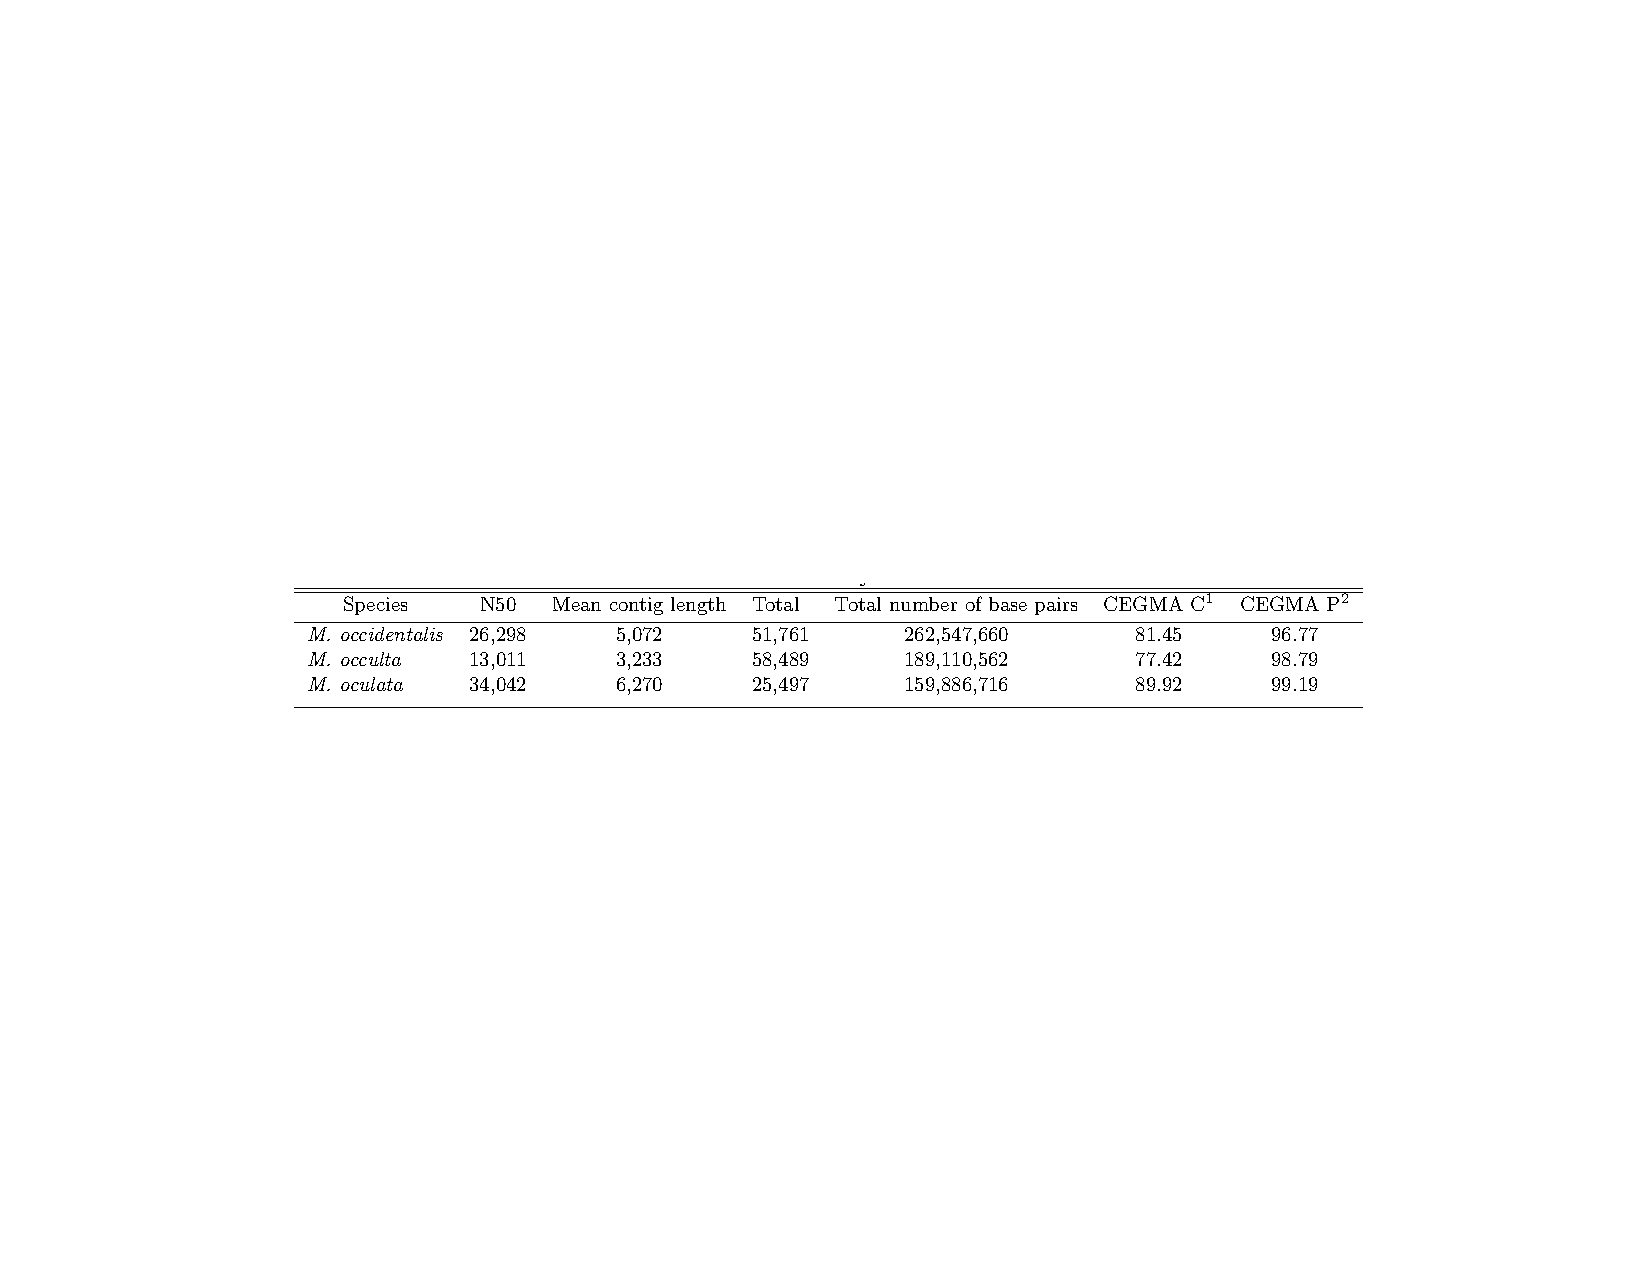
\includegraphics[width=\linewidth]{figures/genome_table_1}
\caption{\textbf{Genome assembly statistics.} The contig N50 length, mean contig length, total number of contigs, total number of base pairs and CEGMA scores were collected for each draft assembly. The CEGMA score is a metric of completeness measured against highly conserved eukaryotic genes. Alignments of 70\% or greater of the protein length are called complete (C) and all other statistically significant alignments are called partial (P).}
\label{table:genome_table}
\end{table}

In addition to N50 lengths, we also used CEGMA (Core Eukaryotic Genes Mapping Approach) scores, in order to evaluate the assemblies' representative completeness \cite{parra_cegma:_2007}. CEGMA reports scores for complete and partial alignments to a subset of core eukaryotic genes. An alignment is considered ``complete'' if at least 70\% of a given protein model aligns to a contig in the assembly, while a partial alignment indicates that a statistically significant portion of the protein model aligns. The partial alignment scores are \mytilde97\% or higher for all assemblies. \textit{M. oculata} has the best complete alignment score at \mytilde90\%. \textit{M. occidentalis} and \textit{M. occulta} have complete alignment scores of 81\% and 77\% respectively (Table~\ref{table:genome_table}). These scores indicate that our assemblies contain at least partial sequences for the vast majority of protein-coding genes in the genomes of these species.
Various factors make it unreliable to predict genome size and gene density based on assembly metrics alone \cite{bradnam_assemblathon_2013}. Of the handful of sequences we isolated and analyzed, we found that the sizes of introns and upstream regulatory regions were roughly comparable to those from their \textit{Ciona} orthologs. This suggests that the \textit{Molgula} genomes may be as compact as the \textit{C. intestinalis} genome (i.e., \mytilde150-170 Mb, \mytilde16,000 genes) \cite{laird_chromatid_1971,simmen_gene_1998,satou_improved_2008}.

\subsection{Gene complexes}
\textit{Hox} genes are a subset of the homeobox genes and are known to be involved with the establishment of morphological identities along the anteroposterior axis of bilaterians and cnidarians \cite{finnerty_origins_2003}. All \textit{hox} genes have a highly conserved 60 amino acid (aa) homeobox sequence \cite{mcginnis_homologous_1984,gehring_homeodomain-dna_1994} and \textit{hox} genes are distinguished by variation of the homeobox domain. There are 4 \textit{HOX} clusters in humans totaling in 39 genes. Within tunicates, \textit{C. intestinalis}, \textit{Halocythia roretzi} and \textit{Oikopleura dioica} \textit{hox} genes have been characterized. \textit{C. intestinalis} has 9 \textit{hox} genes, \textit{Hox1} through \textit{6}, \textit{Hox10}, and \textit{Hox12-13} \cite{dehal_draft_2002}. The \textit{hox} gene of \textit{C. intestinalis} were initially found on 5 scaffolds spanning \mytilde{980} kb using the draft assembly, with \textit{hox2-4}, \textit{hox5-6} and \textit{hox12-13} being found on the same scaffold and later identified to be two clusters of \textit{hox} genes across two chromosomes \cite{ikuta_ciona_2004}. \textit{O. dioica} also has 9 \textit{hox} genes, \textit{hox1-2, hox4}, a duplicate \textit{hox9}, and \textit{hox10-13}, however, none of the genes have been found on the same scaffold, even using a 250 kb window \cite{siok_biological_2004}. 

Eight \textit{hox} genes have be found in \textit{M. occulta} and \textit{M. oculata}, while nine have been found in \textit{M. occidentalis}. The eight found were \textit{Hox1}, \textit{hox2}, \textit{hox3-4}, \textit{hox5}, \textit{hox10} and \textit{hox12-13}, with \textit{hox3} and \textit{hox 4} being found on the same contig in all three species (Figure~\ref{fig:hoxcluster}). Additionally \textit{hox10}, and \textit{hox12-13} are found on the same contig in \textit{M. oculata} with only \textit{hox12-13} being found on the same contig in \textit{M. occidentalis}. However, it appears that the \textit{hox} genes have been rearranged in \textit{M. oculata}, since \textit{hox10} is downstream of \textit{hox12-13}.  \textit{M. occidentalis} had one additional \textit{hox} gene compared to \textit{M. occulta} and \textit{M. oculata}, a duplicate \textit{hox10} gene \mytilde12kb apart found on the same contig. Also, the \textit{M. occidentalis} \textit{hox2} has a stop codon located in the 3-4 helix, although this may be specific to the animal examined and not the total population. The second \textit{hox10} sequence was not fully sequenced, missing 14 aa of the homeobox domain, and the identity of the two sequences was 52.1\% at a nucleotide level, 53.4\% at a protein level, and 91.3\% identical within the homeobox domain (Figure~\ref{fig:occihox10}). \textit{M. occulta}, \textit{M. oculata}, and \textit{M. occidentalis hox} genes span across 7, 5 and 6 contigs respectively and are 197 kb, 311.7 kb and 279 kb in length, respectively.  This is more compact than the \textit{Ciona} \textit{hox} cluster which exhibits longer than usual intergenic regions, averaging in the 5Mb range, when typically the \textit{hox} genes have 100-120 kb intergenic regions separating them \cite{mcginnis_homeobox_1992}. The \textit{hox} gene in the \textit{Molgula} had far smaller intergenic regions, 10-25 kb in length for the \textit{hox} genes that were found on the same contigs.  

\begin{figure}[tbp]
\centering
\includegraphics[scale=0.65]{figures/hox.pdf}
\caption{\textbf{Hox clusters for \textit{M. occulta}, \textit{M. oculata} and \textit{M. occidentalis}} Eight \textit{hox} genes were found in  \textit{M. occulta} and \textit{M. oculata}, while nine were found in \textit{M. occidentalis}. \textit{Hox1}, \textit{hox2}, \textit{hox3-4}, \textit{hox5}, \textit{hox10} and \textit{hox12-13} were found in all three \textit{Molgula} species. \textit{Hox3-4} was found on the same contig in all species, with \textit{hox12-13} found on the same contig in \textit{M. occidentalis} and \textit{M. oculata}. *\textit{M. occulta} \textit{hox12-13} is not found on the same contig, but when aligned using mVista, there is high sequence similarity, showing the possible placement of \textit{hox12-13} in \textit{M. occulta}. \textsuperscript{+}\textit{M. occidentalis} \textit{hox2} gene had a stop codon found in the 3-4 helix. \textsuperscript{\#} numbers correspond to gene color, and rearrangements have been found in \textit{Ciona} and \textit{Molgula}.}
\label{fig:hoxcluster}
\end{figure}

\subsection{Divergence of GRN}
Our sequencing efforts revealed extreme genetic divergence not only between \textit{Ciona} and \textit{Molgula}, as expected, but even within the Molgulids. For example, in Stolfi et al., \cite{stolfi_divergent_2014} we used BLAST to identify the \textit{Molgula} orthologs of \textit{C. intestinalis Mesp}. %(\textit{Ciinte.Mesp}, as per the proposed tunicate gene nomenclature rules, see Stolfi et al., \cite{stolfi_guidelines_2014}). 
\textit{C. intestinalis Mesp} is the sole ortholog of vertebrate genes coding for \textit{MesP} and \textit{Mesogenin bHLH} transcription factor family members \cite{satou_improved_2008}. VISTA alignment shows high sequence similarity between sequences 5' upstream of the \textit{Mesp} genes from the closely related \textit{M. oculata} and \textit{M. occulta}. However, there is no conservation of \textit{Mesp} DNA sequences, coding or non-coding, between \textit{M. oculata}/\textit{occulta} and \textit{M. occidentalis}, nor between \textit{C. intestinalis} and any of the three \textit{Molgula} species. In previous phylogenetic surveys, \textit{M. occidentalis} has been placed as an early-branching \textit{Molgula} species, often grouped together in a subfamily with species ascribed to the genera Eugyra and Bostrichobranchus instead \cite{hadfield_multiple_1995,huber_evolution_2000,tsagkogeorga_updated_2009}. Our sequencing results support the view that \textit{M. occidentalis} is highly diverged from other \textit{Molgula} species.

This sequence divergence is also evident when analyzing the \textit{hox} genes. When comparing sequence similarity of the \textit{hox} genes that were found on the same contigs (\textit{hox3-4} and \textit{hox12-13}), only regions clustered around the coding region for \textit{M. occulta} when compared to \textit{M. oculata} showed similarity, and only coding sequences showed similarity in \textit{M. occidentalis} when compared \textit{M. oculata} (Figure~\ref{fig:hox12}). This sequence similarity was a lot less obvious when comparing \textit{M. occulta} to \textit{M. occidentalis}. However, because of a lack of synteny outside of coding regions between \textit{M. occidentalis} and \textit{M. oculata} we were able to identify \textit{distal-less}, downstream of \textit{Hox13}, which is expressed in endodermal strand cells in \textit{Ciona}.

\begin{figure}[tbp!]
\centering
\includegraphics[scale=0.6]{figures/F1_large.jpg}
\caption{\textbf{The B7.5 lineage in \textit{M. occidentalis}} (A) Diagram comparing \textit{M. occidentalis} (top) and \textit{C. intestinalis} (bottom) embryogenesis at 24�C. Embryos were stained with Alexa Fluor dye-conjugated phalloidin to visualize cell outlines and DAPI to visualize cell nuclei. (B) Diagram of mVISTA (\cite{frazer_vista:_2004}; genome.lbl.gov/vista/) alignment of \textit{M. oculata Mesp (Moocul.Mesp)} locus to orthologs in \textit{M. occulta}, \textit{M. occidentalis}, and \textit{C. intestinalis}. Shaded peaks indicate sequence conservation above 70\% over 100-bp windows (blue = protein-coding, pink = non-coding). Arrows indicate direction of transcription of protein-coding genes. Non-coding sequences upstream of \textit{Mesp} are only conserved between \textit{M. oculata} and \textit{M. occulta}. \textit{M. occidentalis} and \textit{C. intestinalis} show considerable divergence even in protein-coding sequences. Note that microsynteny with SLC5A-related gene supports the orthology of these sequences among the Molgulids.}
\label{fig:mesp}
\end{figure}
\addtocounter{figure}{-1}
\begin{figure}[t]
  \caption{(C) In situ hybridization (ISH) for \textit{Moocci.Mesp} in 110-cell stage embryo (vegetal view), showing mRNA detection (green) in B7.5 blastomeres. Nuclei were counterstained with DAPI (blue). Staging is given by hours post-fertilization (hpf). (D) Vegetal view of a 110-cell stage embryo electoporated with \textit{Moocci.Mesp}>GFP reporter construct. Reporter gene expression was detected by ISH for GFP transcripts (green). Nuclei were stained with DAPI (blue). (E) Lateral view of a mid-tailbud stage embryo electroporated with Moocci. Mesp$>$Histone2B::GFP reporter construct. GFP fluorescence reveals B7.5 descendants on left side of embryo: two trunk ventral cells (TVCs) and two anterior tail muscles (ATMs). (F) Diagram of B7.5 lineage divisions from 110-cell stage to mid-tailbud stage, inferred from previous C. intestinalis studies. Cells are named according to Conklin's method (Conklin, 1905). The lineage is bilaterally symmetric, but only cells on the left side are indicated and named. Relative staging given for \textit{M. occidentalis (Mo.occi)} and \textit{C. intestinalis (Ci.inte)}. 110-cell and late gastrula: vegetal view. Initial tailbud: dorsal view. Mid-tailbud: lateral view. Anterior pole is on the left in all images and illustrations.
DOI: 10.7554/eLife.03728.003}% Continued caption
\end{figure}

\section{Expression of the \textit{M. occidentalis Mesp} gene marks the B7.5 cells}
Ciinte.Mesp specifies the B7.5 cells as the sole progenitors of the cardiopharyngeal lineage \cite{satou_ascidian_2004,davidson_uncoupling_2005,hirano_developmental_1997,stolfi_early_2010}. We performed RNA in situ hybridization (ISH) for \textit{M. occidentalis Mesp (Moocci.Mesp)} and found that this gene is also expressed only in the B7.5 cells of {\em M. occidentalis} embryos (Figure~\ref{fig:mesp}C). These cells are unequivocally identified due to the perfect conservation of early embryonic cell cleavage patterns in all ascidians. ISH for the \textit{M. occulta Mesp} gene (\textit{Mooccu.Mesp}) also revealed conserved expression in this tail-less species (Figure~\ref{fig:mesp}). We successfully adapted the Ciona electroporation protocol for simultaneous transfection of reporter gene plasmids into hundreds of synchronized {\em M. occidentalis} embryos (Figure~\ref{fig:mesp}D,E). We were also able to electroporate {\em M. occulta} embryos (Figure 1?figure supplement 2B). However, only \textit{M. occidentalis} was routinely available to us for in vivo studies, so we focused our experiments on this species. Development of \textit{M. occidentalis} embryos was optimal at 24�C and faster than that of \textit{C. intestinalis} (Figure~\ref{fig:mesp}A). Using electroporation-based transfection, we determined that an \mytilde1.1 kb genomic DNA fragment upstream of \textit{Moocci.Mesp} is able to drive expression of fused reporter genes specifically in the B7.5 cells with no `leaky' expression in other cells as is commonly observed in \textit{C. intestinalis} (Figure~\ref{fig:mesp}D; \cite{stolfi_genetic_2012}). This faithful recapitulation of \textit{Moocci.Mesp} expression and the persistence of GFP allows for visualization of the descendants of B7.5 long after endogenous Moocci.Mesp transcription has ceased (Figure 1?figure supplement 3; Davidson et al., 2005). At the tailbud stage, we find that each B7.5 blastomere gives rise to four grand-daughter cells (Figure~\ref{fig:mesp}E). The two anterior B7.5 grand-daughter cells on either side of the bilaterally symmetric embryo migrate anteriorly and are termed the trunk ventral cells (TVCs) due to their final position in the \textit{C. intestinalis} and \textit{H. roretzi} embryos \cite{nishida_cell_1987}. Their posterior sister cells remain in the tail and become anterior tail muscles (ATMs). As far as we can tell, B7.5 lineage ontogeny is perfectly conserved between \textit{M. occidentalis} and \textit{C. intestinalis} (Figure~\ref{fig:mesp}F).

\section{Divergence of Mesp cis-regulatory sequence function between \textit{M. occidentalis} and \textit{C. intestinalis}}
Given the obvious parallels between \textit{C. intestinalis} and \textit{M. occidentalis} cardiopharyngeal development, we expected transcriptional regulatory mechanisms to also be highly conserved between the two species. We tested this assumption by electroporating \textit{C. intestinalis} reporter constructs into \textit{M. occidentalis} embryos, and vice-versa. We observed that a \textit{Ciinte.Mesp} reporter construct \cite{davidson_uncoupling_2005}, when electroporated into \textit{M. occidentalis} embryos, drives relatively weak reporter gene expression in B7.5 with substantial leaky expression in other tissues (Figure~\ref{fig:tbx}A). Conversely, the Moocci.Mesp enhancer fails to drive any reporter gene expression when electroporated into \textit{C. intestinalis} embryos (Figure~\ref{fig:tbx}B), despite recapitulating robust B7.5-specific expression in \textit{M. occidentalis} embryos (Figure~\ref{fig:mesp}D,E). These data suggest acute DSD of transcriptional regulatory mechanisms underlying otherwise identical \textit{Mesp} expression patterns. More specifically, the trans-regulatory environment of the B7.5 blastomeres has diverged between Molgula and Ciona, and compensatory changes in the respective \textit{Mesp} cis-regulatory sequences must have rendered these unable to function adequately outside of that milieu.

The observation of \textit{Mesp} incompatibility or unintelligibility, lead to the examination of Foxf cis-elements, who is also involved in TVC specification, both revealed divergent cis-regulatiory logic for underlying identical gene expression patterns. This sparked an interest to see if there was a general trend of cis-regulatory unintelligibility between \textit{C. intestinalis} and \textit{M. occidentalis}. This revealed that \textit{M. occidentalis Tbx6} we found that the Ciinte.Hand-r reporter can drive reporter gene expression in M. occidentalis TVCs. Thus, unlike the case of Foxf, there is an asymmetric intelligibility of Hand-r TVC enhancers between M. occidentalis and C. intestinalis. Moreover, a M. oculata Hand-r TVC enhancer is functional in M. occidentalis but not in C. intestinalis Taken together, these data suggest that differences in enhancer logic may have accumulated over the course of the deep evolutionary history between Molgula and Ciona but not between M. occidentalis and M. oculata, and that some enhancers may have evolved asymmetrically in the two branches, retaining greater pan-ascidian ``intelligibility'' in one or the other.

\begin{figure}[tbp!]
\centering
\includegraphics[scale=0.6]{figures/F14_large.jpg}
\caption{\textbf{The B7.5 lineage in \textit{M. occidentalis}}Cross-species reporter construct assays reveal multiple cases of cis-regulatory unintelligibility. (A) C. intestinalis embryo electroporated with Ciinte.Tbx6-r.b$>$GFP reporter construct \cite{christiaen_spatio-temporal_2009}, which drives GFP expression in tail muscles and the B7.5 lineage cells (arrowheads), recapitulating endogenous Ciinte.Tbx6-r.b expression. (B) M. occidentalis embryo electroporated with Moocci.Tbx6-r.b$>$GFP reporter construct, which recapitulates expression in tail muscle cells including B7.5 lineage cells (arrowheads). (C) C. intestinalis embryo electroporated with Moocci.Tbx6-r.b$>$GFP, which drives expression in B-line tail muscle and mesenchyme cells but is excluded from the B7.5 lineage. (D) C. intestinalis embryo electroporated with Ciinte.Hand-r$>$H2B::GFP reporter (Davidson and Levine, 2003), which drives H2B::GFP expression in anterior endoderm, A7.6 lineage, and TVCs (arrowheads), recapitulating endogenous Ciinte.Hand-r expression. (E) M. occidentalis embryo electroporated with Moccci.Hand-r$>$H2B::GFP construct, which recapitulates the same expression pattern. (F) C. intestinalis embryo electroporated with Moocci.Hand-r$>$H2B::GFP, which drives expression in endoderm and A7.6 lineage, but not in B7.5. (G) M. occidentalis embryo electroporated with Ciinte.Ebf neuron-specific YFP (green) and H2B::mCherry (red) reporter constructs electroporated \cite{stolfi_neuronal_2011}, which drive very weak expression in a limited subset of motor ganglion neurons (green and red).}
\end{figure} 
%\addtocounter{figure}{-1}
\begin{figure}[t]
\ContinuedFloat
%\captionsetup{list=off,format=cont}
\caption{(H) C. intestinalis embryo electroporated with a Moocci.Ebf$>$YFP reporter, which drives robust reporter gene expression in several brain, motor ganglion, and nerve cord neurons. (I) C. intestinalis embryos electroporated with Ciinte.Sox1/2/3 (left) and Moocci.Sox1/2/3 (right) H2B::mCherry reporter constructs, both of which recapitulate Sox1/2/3 expression in ectoderm. Panels A?F are lateral views of tailbud embryos, panels G is a dorsal view of a tailbud embryo, panel H is a dorso-lateral view of a hatched larva, and panel I shows vegetal views of mid-gastrula stage embryos. Anterior is to the right, except in Panel I, in which anterior is to the top. DOI: 10.7554/eLife.03728.023}
\label{fig:tbx}
\end{figure}

\section{Discussion}
Three \textit{Molgula}\textemdash\textit{M. occulta}, \textit{M. oculata} and \textit{M. occidentalis}\textemdash species have been sequenced and assembled; these are the first of any molgulids to have assembled genomes. Developmentally the three species are very similar up to the gastrula stage, where \textit{M. occulta} diverge from the typical solitary ascidian body plan and develop without a tail \cite{berrill_studies_1931,nishida_cell_1987}. 

In vertebrate and other bilaterians the \textit{hox} genes has been shown to be important for patterning along the anterior-posterior axis \cite{finnerty_origins_2003,mallo_regulation_2013}. The same has not been shown in ascidians, where \textit{hox} has more of a tissue specific role \cite{ikuta_limited_2010}.  \textit{Ciona} has 10 \textit{hox} genes and is missing \textit{hox7-9} and \textit{11}, with \textit{hox10} and \textit{12} being the only two genes to show morphological effects when knocked down. \textit{Hox10} is involved in the regulation of the motor neuron differentiation and \textit{hox12} is involved in tail development, through the elongation of the posterior most section of the tail and of the epidermal cells at the tail tip \cite{ikuta_limited_2010}. We observed the absence of \textit{hox6} in all three \textit{Molgula} species, which is not surprising, seeing that \textit{hox6} is also missing in \textit{O. dioica} and no expression is detected in \textit{C. intestinalis} through whole mount in situ hybridization at any stage of development \cite{ikuta_ciona_2004,seo_hox_2004}. No two of the \textit{Molgula} species show the same \textit{hox} cluster and all show a strong divergence outside of coding regions, even more so in \textit{M. occidentalis}. There is a duplication of \textit{M. occidentalis hox10} which could lead to a split in function since \textit{Ciona Hox10}  is expressed in two region during the mid-tailbud stage\textemdash a small region of the anterior nerve cord, and a small area of the posterior ventral endoderm and adjacent tissue \cite{ikuta_ciona_2004}. It is proposed that ascidians evolved their simple body plans and rapid embryogenesis through extensive genomic rearrangement and gene loss, with specific loss of several \textit{hox} genes \cite{ikuta_organization_2005}. \textit{Hox12-13} are not found on the same contig in \textit{M. occulta}, however when aligned with mVista there appears to be a strong case for synteny (Figure~\ref{fig:hox12}), so it is possible they are clustered, but the contigs are not joined because the \textit{M. occulta} genome assembly is too fragmented. \textit{Hox} function does not have the same level and so far their has not been a consistence between \textit{hox} clusters in no Tunicate studied, showing that \textit{hox} is tends do be divergent within the tunicates.

In \textit{Ciona} \textit{dll} stains in the endodermal strand cell during early-tailbud embryos, showing positive signals in two cells of the endodermal strand \cite{caracciolo_identification_2000} which derives from the primary muscle or mesenchyme lineage \cite{rossomando_morphogenesis:_1992}, while in Drosophila embryos \textit{dll} is required for the gene pathway for limb formation in the thoracic segment \cite{vachon_homeotic_1992}. Because of the lack of homology outside of coding regions, we were able to identify \textit{distal-less} (\textit{dll}) downstream of \textit{hox13} in both \textit{M. occidentalis} and \textit{M. oculata}, but we did not find it in \textit{M. occulta}.  Further investigation is needed, as this could potentially be tied to failed muscle cell differentiation in \textit{M. occulta}.

From our initial survey of a handful of enhancers from {\em C. intestinalis}, {\em M. occidentalis}, and {\em M. oculata}, we encountered several instances of either mutual unintelligibility, or asymmetric intelligibility of enhancers. These results add to the mounting evidence suggesting that acute and pervasive DSD may have occurred over the course of ascidian evolution, obfuscated by the identical cell lineages and highly conserved gene expression patterns of ascidian embryos \cite{swalla_protochordate_2004}. The multiple examples of cis-regulatory unintelligibility we identified were rather unexpected given (a) the extremely conserved pattern of expression of orthologous genes from Molgula and Ciona \cite{takada_expression_2002} and (b) previous observations of mutual intelligibility of enhancers between C. intestinalis and H. roretzi (e.g., Otx), and between C. intestinalis and the more closely related C. savignyi \cite{johnson_noncoding_2004,brown_functional_2007}. Large-scale, quantitative cross-species assays and detailed GRN studies will illuminate factors that may contribute to conservation or divergence in regulatory mechanisms.

\section{Conclusion}
\textit{Hox} genes function is not conserved within the tunicates, which have also undergone substantial \textit{hox} gene loss. All central \textit{hox} genes are missing in all three \textit{Molgula} species. Studying these three molgula species have compounded the evidence that Tunicate has lost both \textit{hox7} and \textit{hox8} after diverging from the vertebrate and cephalochordate lineages, while ascidians have lost \textit{hox9} and \textit{hox11} after diverging from the larvaceans. It appears because \textit{hox} does not act as an anterior-posterior organizer in ascidians, \textit{hox} genes are more easily lost in ascidians and other genes have taken over this role. 

Although tunicates have a well defined and invariant cleavage, the mechanism behind development is not always the same from species to species. % We have demonstrated that tunicates with the same different \textit{M. occidentalis} has shown. 
We speculate that a high frequency of compensatory changes, required for the rapidly evolving ascidians to accommodate the constraints imposed by their invariant embryonic cell lineages and highly compact genomes, has given rise to a preponderance of cross-species cis-regulatory unintelligibility,
following the DSD/SPC model. This perfect storm of intrinsic factors may be the key to
explaining the dichotomy observed between highly conserved embryos and divergent cis-regulatory
structure/function in ascidians.

\chapter{Differential expression analysis of tail loss in an invertebrate chordate}

\section{Introduction}

Chordates are composed of three subphyla\textemdash vertebra, tunicata and cephalochordata\textemdash that all share several characteristics, with the notochord being the key characteristic (from which the phylum name comes). The tail development of larvaceans such as Oikopleura dioica and several species of ascidians and tunicates has been well studied \cite{jeffery_factors_1992,nakatani_mutations_1999,kugler_evolutionary_2011}. Larvaceans form tailed larvae with a hollow dorsal notochord and keep their tail throughout their adult life stage. Ascidians generally form their tail in a similar manner before undergoing the process of metamorphosis, in which the larval tail is absorbed in to the trunk region \cite{paris_history_2008}. A typical ascidian larvae tail forms through the convergence, intercalation and extension of the notochord and the differentiation of the posterior muscle cells \cite{swalla_mechanisms_1993}. When fully formed the ascidian notochord contains 40 cells, flanked by three rows of muscle cells. The ancestral notochord or notochord-like structure is believed to have been muscle based, which is perhaps the reason that the tail formation is often contingent upon proper development of both notochord and muscles \cite{lauri_development_2014}. This idea is supported by the observation that the primary and secondary notochord and muscle lineage are derived from the same blastomere, and the ascidian tail needs both the notochord and differentiated muscle to form a larval tail \cite{nishida_cell_1987,di_gregorio_tail_2002}.

Of the \mytilde3000 species of ascidians fewer than 20 do not form a tail, with the majority being Molgulidae species \cite{berrill_studies_1931,huber_evolution_2000}. This likely represents several independent instances of evolutionary loss of the tail, and introduces the question of why are the Molgulidae so susceptible to tail-loss. Although the mechanism behind tail-loss differs by species, a common characteristic is the lack of a notochord that intercalates and extends, as well as a less differentiated central nervous system (CNS) structures and tail muscles \cite{swalla_mechanisms_1993}. \textit{Molgula bleizi} notochord cells converge to the midline, and began to extend, but cells never properly intercalate and the tail formation stops before it is fully formed \cite{jeffery_evolution_1999}. In \textit{M. bleizi} there is an early down-regulation of \textit{brachyury} (\textit{bra})\textemdash a key notochord inducer\textemdash and larva-specific muscle actin genes have become pseudo genes \cite{jeffery_evolution_1999}.   

A similar situation is observed in \textit{Molgula occulta}: muscle actins have become pseudogenes, independently of their conversion in \textit{M. bleizi}. \textit{M. occulta} and \textit{Molgula oculata} are two closely related species, who in their adult form are virtually identical, with the exception of a white pigment spot between the two siphons of the tailed species, \textit{M. oculata}. During development the species are indistinguishable up to the gastrula stage. In late gastrula when the notochord and muscle progenitor begin to move posteriorly \cite{swalla_novel_1993} and the notochord begins to form, the morphological divergence becomes evident. Through subtractive screening Swalla and Jeffery \cite{swalla_requirement_1996} have identified \textit{manx}, a zinc finger transcription factor (TF) and the cytoskeletal protein p58 to be down-regulated in \textit{M. occulta} relative to \textit{M. oculata} \cite{swalla_identification_1991}, amongst other genes were shown to be one of the causes of the tail loss in \textit{M. occulta}. There are several steps that take place to form the notochord and tail: first, the notochord cells move mediolaterally to the midline; and next, the cells polarize and intercalate, changing their shape and extending posteriorly \cite{keller_mechanisms_2000, jiang_ascidian_2005,stemple_structure_2005}. This process is known as convergence and extension. Although the two species have different developmental programs, crossing the tail-less \textit{M. occulta} eggs with sperm of the tailed \textit{M. oculata} produces a hybrid with 20 notochord cells like the tail-less species, but in which the cells intercalate and extend like the tailed species. In the hybrids the expression of \textit{manx} and p58 are restored, and antisense phosphorothiated oligodeoxynucleotide \textit{manx} in the hybrids have shown that zygotic \textit{manx} is necessary for tail formation \cite{swalla_requirement_1996}.

Several key tail development genes have been identified as present in the \textit{M. occulta} genome, but expressed at low levels during embryogenesis, and when expressed, some of these genes were shown to restore features in the hybrid \cite{swalla_interspecific_1990,jeffery_factors_1992,swalla_novel_1993, swalla_requirement_1996}. With advances in high throughput sequencing technologies, gene expression of \textit{M. occulta}, \textit{M. oculata}, and hybrid species can be analyzed on a whole transcriptome level \cite{gyoja_analysis_2007,pickrell_variation_2010}. mRNA of three different developmental stages for \textit{M. occulta}, \textit{M. oculata}, and their hybrid has been sequenced and assembled at Michigan State University (MSU). These three transcriptomes were used to % identify the presence or absence 
assess the expression levels of known notochord genes downstream of \textit{bra} using \textit{C. intestinalis} data from the NCBI database (\url{ncbi.nlm.nih.gov}). BLAST searches were done against known notochord genes, and several of them were selected for further analysis, including \textit{FGF9/16/20}, \textit{prickle (pk)}, and several other downstream genes.  These genes were then used to construct a putative \textit{brachyury} gene regulatory network for both \textit{M. occulta} and \textit{M. oculata}. 

\section{Methods}
\subsection{Sample collection, sequencing and assembly}
RNA was extracted from all three \textit{Molgula} species using the methods discussed in Lowe et al. \cite{lowe_evaluating_2014}. RNAs for the gastrula (3hpf), neurula (4hpf) and mid-tailbud (6hpf) stages were extracted for both \textit{M. occulta} and \textit{M. oculata}, with a replicate for the gastrula and a sample for early-tailbud stage sequenced from \textit{M. occulta}. %Samples from a fertilized embryo, tailbud and larvae were sequenced for \textit{M. occidentalis} to gain a broad scope of expression.
DNA was extracted from the gonads of an individual adult specimen for %\textit{M. occidentalis},
\textit{M. occulta}, and \textit{M. oculata}. Two paired-end jumping libraries were collected for each species ranging from \mytilde300bp to \mytilde950bp. Further details about extraction methods and libraries can be found in Stolfi et al., \cite{stolfi_divergent_2014}. Sequencing for \textit{M. occulta} and \textit{M. oculata} RNA were conducted at the Michigan State University, while all other sequencing was done at New York University. All libraries were paired-end, with 75 base pair (bp) reads for the sequencing done at MSU and 100 bp reads for the NYU sequencing. 

Genome assemblies were conducted using 3-pass digital normalization \cite{brown_reference-free_2012} and assembled using Velvet\cite{zerbino_velvet:_2008}. Other assemblers were tested, however, Velvet produced the best results with the least fragmented assemblies. Assemblies were initially done with 21 $\geq$ k $\geq$ 71, for intervals of 10. We selected the 'k' value with the highest N50, and then the genomes were reassembled for a k$\pm$10 with a step size of 2 for the selected assembly, and the best N50 was chosen. A k of 31, and 49 were select for \textit{M. occulta}, and \textit{M. oculata}, respectively. 

Both \textit{de novo} and reference based assemblies were used to create gene models. Reads were mapped to their respective genomes using bowtie2 and tophat to identify genes and alternative splicing variants \cite{langmead_fast_2012,trapnell_differential_2012}. The accepted.bam files were then sorted and indexed using samtools \cite{li_sequence_2009}. The sorted bam files were then processed using cufflinks and cuffmerge to generated consensus gtf annotation files. The digitally normalized trinity \textit{de novo} assembled transcripts from Lowe et al. \cite{lowe_evaluating_2014}, were aligned to their respective genomes using BLAT \cite{haas_novo_2013}. The cufflinks/cuffmerged gtf files were then converted into bed files and merged with the annotation files from the mapped \textit{de novo} assembly aligned using gimme (\url{https://github.com/likit/gimme}). Gimme joins gene models using a graph based method to develop more complete transcripts. The gimme gene models were then converted to gff format using the script bed2gff in the gimme utils folder in order to extract the transcripts from the genome in a multi fast file. Transcripts were then extracted using ``gffread -w transcripts.fa -g /path/to/genome.fa transcripts.gtf'' which is included in the cufflinks package. The extracted transcripts were partitioned into transcript families and annotated using the khmer suite and steps found in the eel-pond protocol (\url{https://khmer-protocols.readthedocs.org/}). \textit{Ciona intestinalis} was used as an annotation reference, and the sequences were retrieved as discussed in Chapter 3. 

\subsection{Gene counts and differential expression analysis}
Reads were mapped to transcripts from the gimme gene models for their respective species. Reads from the hybrids were mapped onto both the \textit{M. occulta} and \textit{M. oculata} transcripts, since the hybrids are F1 hybrids and should contain an allele from each parent. Read counts were generated using eXpress \cite{roberts_streaming_2013}. eXpress gives the option of ``Total counts'' and ``Effective counts'', which reports the number of reads mapped per transcript and the normalized counts based on transcript length, respectively. Because EdgeR uses unnormalized reads, ``Total counts'' were used. Counts for hybrid reads mapped to \textit{M. occulta} and \textit{M. oculata} were combined to calculate total expression at a given stage. A replicate was only provided for one of the samples, 3hpf, and because of this 5hpf was treated as a replicate for 6hpf. These time points correspond to early and mid-tail bud stages in the tailed ascidian. 

Differential expression was calculated using the Bioconductor EdgeR package because of its ability to work with minimal replicates \cite{robinson_edger:_2010}. We ran RBH  for \textit{M. occulta} and \textit{M. oculata} in order to identify orthologous transcripts to conduct allele specific differential expression analysis on the hybrid. We used both estimateGLMCommonDisp and estimateGLMTagwiseDisp to calculate dispersions. There is only a replicate for \textit{M. occulta} gastrula stage (F+3), because of this we used \textit{M. occulta} early tailbud stage as a replicate for the mid tailbud stage. These replicates were used to calculate dispersions for all samples. Exact-test with p = 0.05 were used for differential expression, and transcripts with false discovery rate (FDR) of 0.05 being called as differentially expressed. 

\section{Results}
\subsection{\textit{M. occulta} and \textit{M. oculata} have strong overlap in gene expression}
\textit{C. intestinalis} is the closest ascidian species with a well annotated genome, and so we used \textit{Ciona} proteins obtained from the NCBI to annotate the genomes of both \textit{M. occulta} and \textit{M. oculata}. Reciprocal best hit (RBH) blast with an e-value of 1e-3, were done with the \textit{M. occulta} and \textit{M. oculata} transcriptomes against \textit{C. intestinalis} for the annotation of both \textit{Molgula} species.  We are aware this is a low threshold for homology, however, information for these species are not known and we wanted to gain as much insight as possible for genes and gene function. Moreover, the reciprocal best hit criterion is extremely stringent.

The gene models for \textit{M. occulta} and \textit{M. oculata} produced 42,365 and 40,775 sequences total, respectively. Precisely 8,627 \textit{M. occulta} transcripts were annotated as orthologs and 22,700 transcripts were annotated as showing homology. Similar annotation numbers were produced with \textit{M. oculata}: 8,677 showed orthology, and 22,583 showed homology. \textit{M. occulta} and \textit{M. oculata} have a high overlap in number of translated transcripts that showed any level of homology with \textit{C. intestinalis} proteins from the NCBI database. Of the 16,414 {\em Ciona} proteins, \textit{M. occulta} had BLAST hits for 83.6\% and 86.5\% had hits in \textit{M. oculata}. \textit{M. occulta} had hits for 453 proteins that were not found in \textit{M. oculata} and \textit{M. oculata} had hits for 921 transcripts that did not have hits in \textit{M. occulta}, yielding an overlap of 97\% in assembled homologs.

\begin{figure}[tbp]
\centering
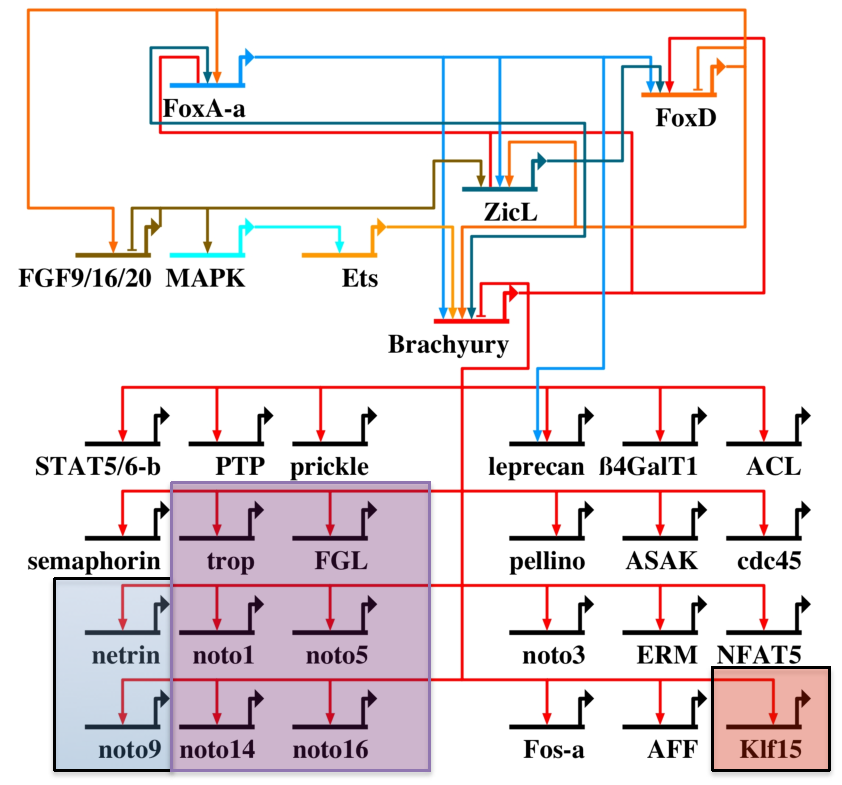
\includegraphics[scale=0.8]{figures/bra_grn.pdf}
\caption{\textbf{\textit{Brachyury gene regulatory network.}}\textit{Bra} is a key notochord inducer, and without its expression neither the notochord nor the chordate tail forms. Downstream genes have been identified in various studies and of these 67 genes 11 were missing from the transcriptomes of both species. The missing genes were \textit{cofilin}, \textit{entactin} (\textit{nidogen-2-like}), \textit{fibrinogen-like protein} (\textit{FGL}), \textit{fibronectin}, \textit{multidom}, \textit{noto1}, \textit{noto5}, \textit{noto14}, \textit{noto16}, and \textit{tropomyosin}. \textit{netrin}, and \textit{noto9} are missing in \textit{M. occulta} and \textit{Klf15} is missing in \textit{M. oculata}. (Blue) missing in \textit{M. occulta}, (Red) missing in \textit{M. oculata}, and (Purple) missing in both species. This GRN was built from previous studies  \cite{hotta_temporal_1999,hotta_characterization_2000,hotta_brachyury-downstream_2007,kugler_evolutionary_2008,kugler_evolutionary_2011}, using the BioTapestry software \cite{longabaugh_visualization_2009}.}
\label{fig:bra_grn}
\end{figure}
\subsection{Notochord gene network}

Next, we examined genes associated with notochord development in \textit{C. intestinalis} to investigate the molecular development of the tail. Gene candidates were identified as being involved in tail formation and notochord development through previous analysis of genes downstream of \textit{bra} \cite{hotta_temporal_1999,hotta_characterization_2000,hotta_brachyury-downstream_2007,kugler_evolutionary_2008,kugler_evolutionary_2011}. From these studies many potential notochord genes were identified; we compiled a list of 67 genes and identified those expressed during the gastrula, neurula or tailbud stages within the %genomes and 
transcriptomes of both \textit{M. occulta} and \textit{M. oculata} (Figure~\ref{fig:bra_grn}). Of the 67 genes, 11 were not expressed in the transcriptomes of either species: \textit{cofilin}, \textit{entactin} (\textit{nidogen-2-like}), \textit{fibrinogen-like protein} (\textit{FGL}), \textit{fibronectin}, \textit{multidom}, \textit{noto1}, \textit{noto5}, \textit{noto14}, \textit{noto16}, and \textit{tropomyosin}. The remaining genes without orthologous sequences were \textit{netrin}, and \textit{noto9} in \textit{M. occulta} and \textit{Klf15} in \textit{M. oculata}. In \textit{Ciona}, \textit{netrin} is expressed in the notochord and the central nervous system and is associated with axon guidance \cite{hotta_characterization_2000}. \textit{Klf15} was detected in the notochord, but there is currently no known information regarding its function \cite{passamaneck_direct_2009}. Taken together, these demonstrates a strong overlap in the presence of the number of genes associated in notochord formation in both \textit{M. occulta} and \textit{M. oculata}.

\subsection{Differential expression between neurula and tailbud appears to be key factor in tail development} 

\begin{landscape}
\begin{table}[b]
%\makebox[\linewidth]{
\begin{center}
\begin{tabular}{l c c c c}
\hline\hline
{\multirow{2}{*}{Species} } & {\multirow{2}{*}{Condition} }&\multicolumn{3}{c}{Number of transcripts that show...} \\ %\cline{1-6}% inserts table %heading
& & Up-regulation & Down-regulation & No differential expression \\ [0.5ex]
\hline
{\multirow{2}{*}{\textit{M. occulta} }} 	&						
from Gastrula to Neurula& 260 & 8 & 20197  \\ 
\multicolumn{1}{ l  }{}                        			&				
from Neurula to Tailbud&1 & 4 & 20460    \\ \cline{1-5}
{\multirow{2}{*}{\textit{M. oculata} }} &
from Gastrula to Neurula& 119 & 66 & 20280  \\ 
\multicolumn{1}{ c  }{}                        &
from Neurula to Tailbud&1170 & 626 & 18669    \\ \cline{1-5}
{\multirow{2}{*}{Hybrid }} &
from Gastrula to Neurula& 21 & 99 & 20345  \\ 
\multicolumn{1}{ c  }{}                        &
from Neurula to Tailbud&1270 & 129 & 19066    \\ 
\hline
\end{tabular}
\caption{Differential expression: Species \textit{vs} time}
\label{table:de}
\end{center}
\end{table}
\end{landscape}

When comparing the tailbud stage to the neurula stage there was essentially no significant differential expression observed in \textit{M. occulta}. A total of 5 genes were said to be differentially expressed (FDR \textless 0.05). However a major shift in differential expression was seen in both \textit{M. oculata} and the hybrid at the tailbud stage relative to the neurula stage (Figure~\ref{fig:de_plots}). There were 1170 and 1270 transcripts up-regulated, and transcripts and 129 transcripts down-regulated in \textit{M. oculata} and the hybrid respectively. That equates to a 10\textit{x} increase in differentially expressed transcripts in both hybrid and \textit{M. oculata} tailbud embryos relative to the respective neurula stage embryos.

\begin{landscape}
\begin{figure}[!H]
	\subfloat[\label{subfig:mocc3v4}]{%
	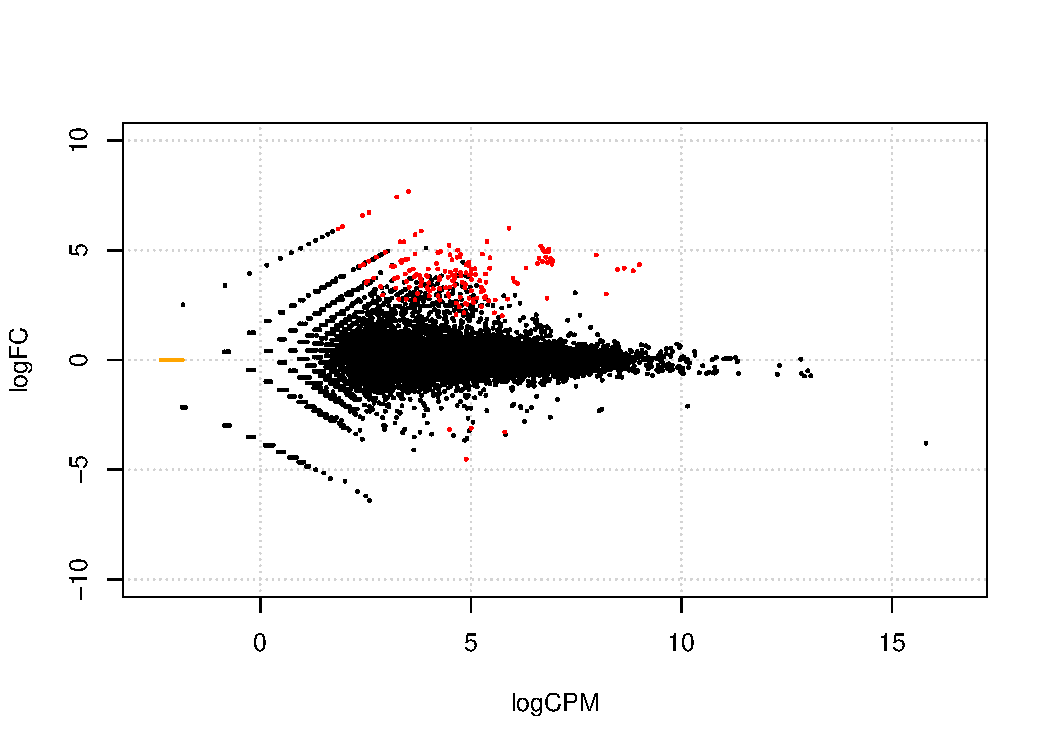
\includegraphics[scale=0.45]{figures/mocc3v4_graph.pdf}
	}
	\subfloat[\label{subfig:mocu3v4}]{%
	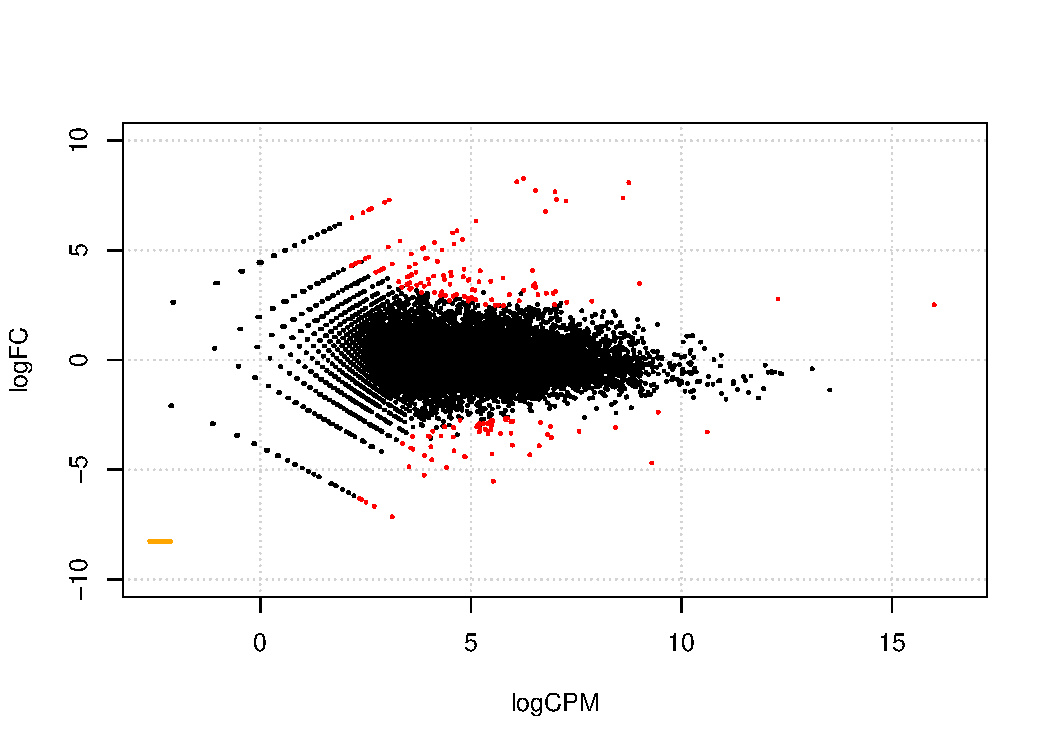
\includegraphics[scale=0.45]{figures/mocu3v4_graph.pdf}
	}
	\subfloat[\label{subfig:hyb3v4}]{%
	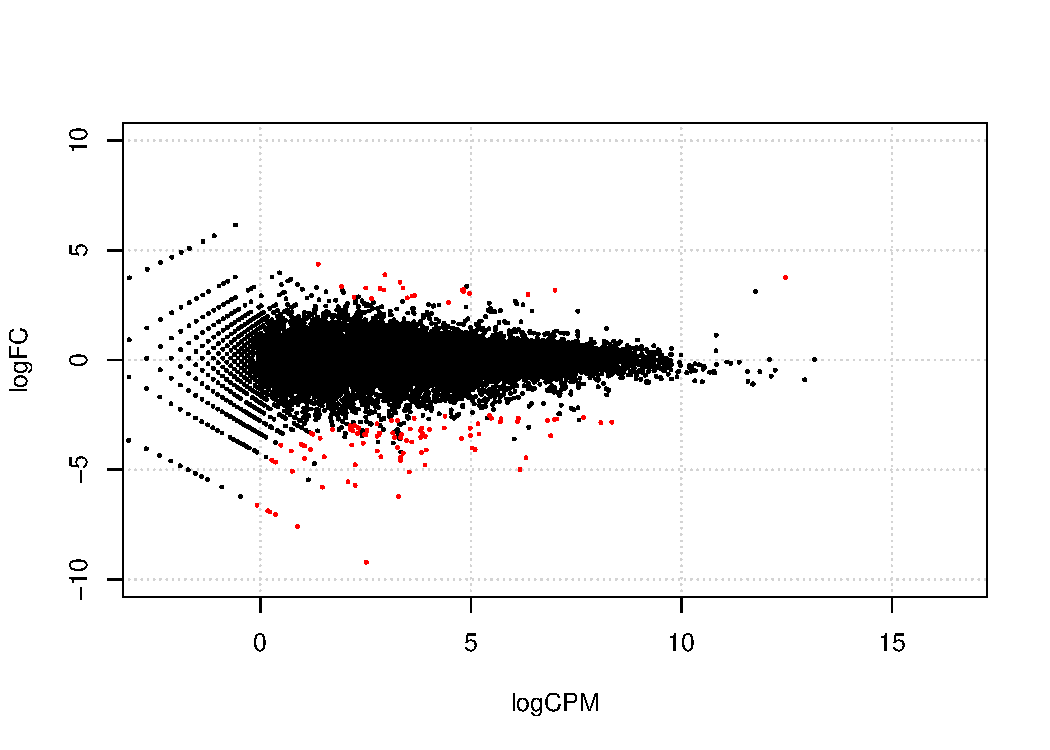
\includegraphics[scale=0.45]{figures/hyb3v4_graph.pdf}
	}
	\hfill
	\subfloat[\label{subfig:mocc4v6}]{%
	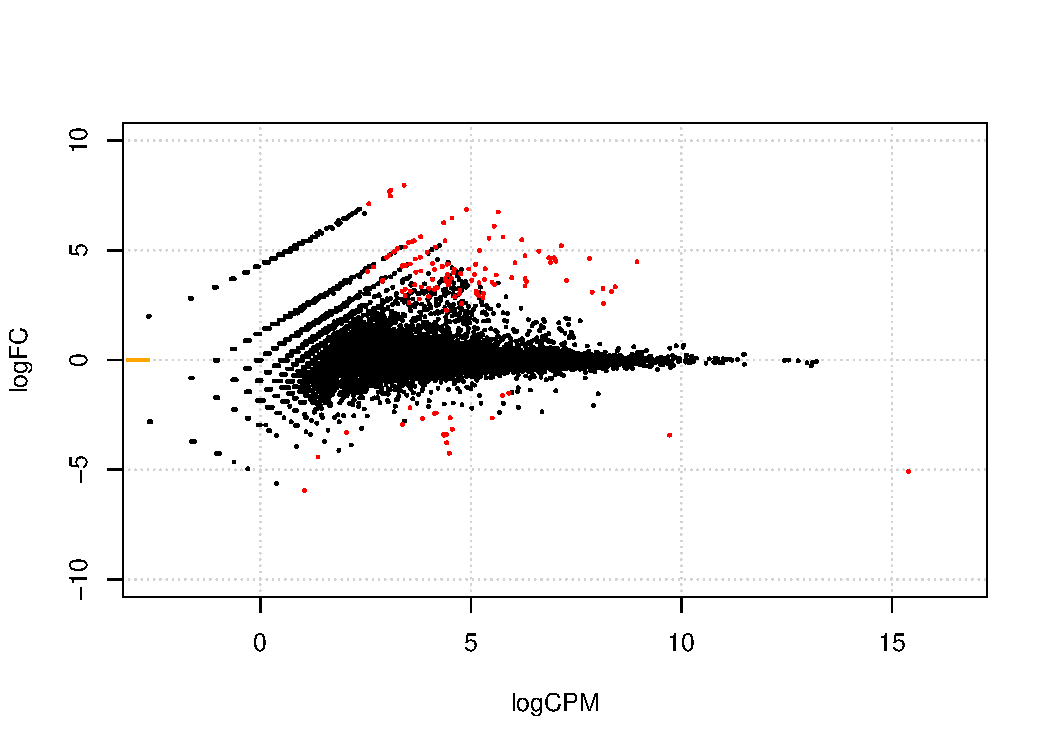
\includegraphics[scale=0.45]{figures/mocc4v6_graph.pdf}
	}
	\subfloat[\label{subfig:mocu4v6}]{%
	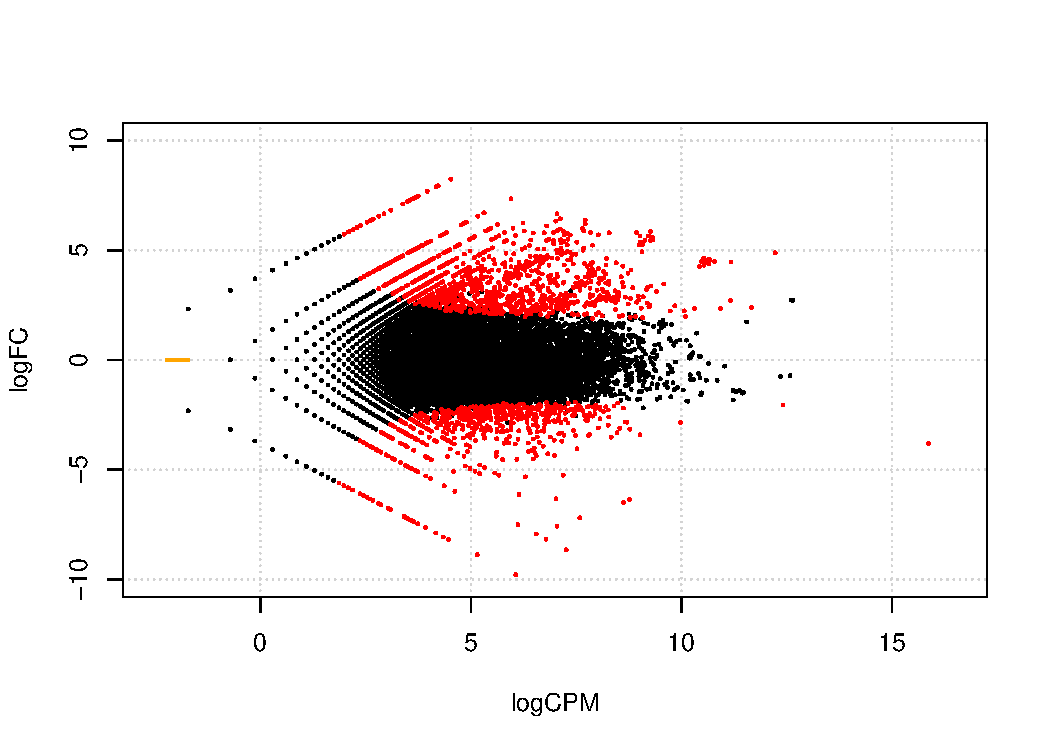
\includegraphics[scale=0.45]{figures/mocu4v6_graph.pdf}
	}
	\subfloat[\label{subfig:hyb4v6}]{%
	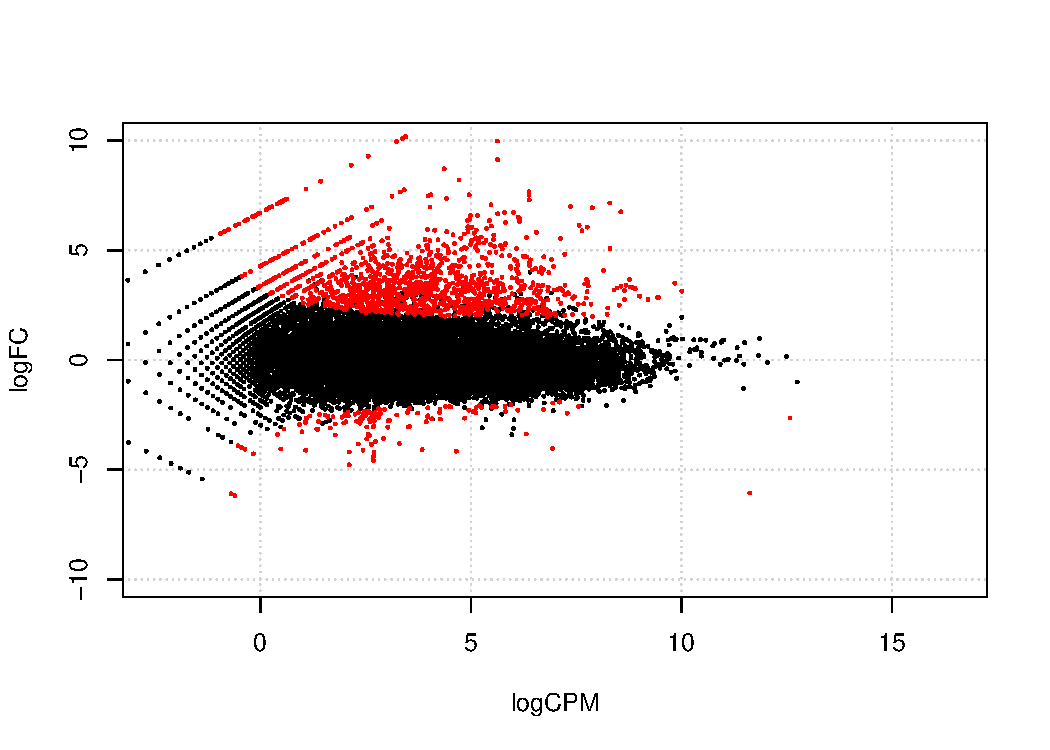
\includegraphics[scale=0.45]{figures/hyb4v6_graph.pdf}
	}
	\caption{\textbf{Differential expression of homologous transcripts.} Differential expression in \textit{M. occulta} for (a) gastrula vs neurula, and (d) neurula vs tailbud, \textit{M. oculata} for (b) gastrula vs neurula, and (e) neurula vs tailbud, and the hybrid for (c) gastrula vs neurula, and (f) neurula vs tailbud. Genes in red are differentially expressed with a FDR \textless 0.05}
	\label{fig:de_plots}
\end{figure}
\end{landscape}

Only \textit{M. occulta} embryos that expressed \textit{manx} and p58 produced hybrids with urodele features. To identify other candidate genes whose differential expression in \textit{M. occulta} may contribute to the tail-less condition, we sequenced and assembled three developmental stages\textemdash gastrula, neurula, and tailbud\textemdash across \textit{M. occulta}, \textit{M. oculata} and their interspecies hybrid. The tail-less species, \textit{M. occulta}, showed the highest level of differential expression (FDR \textless 0.05), with 260 (97\%) of the identified differentially expressed transcripts up-regulated in the neurula stage relative to the gastrula stage. (Table~\ref{table:de}). \textit{M. oculata} also had more transcripts up-regulated (65\%) than down-regulated at the neurula stage relative to the gastrula. Hybrids did not follow this trend; the majority of differentially-expressed hybrid genes are down-regulated at this stage (82\%).  

When comparing the tailbud stage to the neurula stage there was essentially no significant differential expression observed in \textit{M. occulta}. A total of 5 genes were said to be differentially expressed (FDR \textless 0.05). However a major shift in differential expression was seen in both \textit{M. oculata} and the hybrid at the tailbud stage relative to the neurula stage (Figure~\ref{fig:de_plots}). There were 1170 and 1270 transcripts up-regulated, and transcripts and 129 transcripts down-regulated in \textit{M. oculata} and the hybrid respectively. That equates to a 10\textit{x} increase in differentially expressed transcripts in both hybrid and \textit{M. oculata} tailbud embryos relative to the respective neurula stage embryos..

\subsection{Overlap between hybrid and M. oculata alleles}
When comparing transcript expression from neurula to tailbud in \textit{M. oculata} and the hybrid there is a total of 2,440 transcripts up-regulated collectively. Of these 2,440 transcripts, 328 (13\%) overlap (Figure~\ref{subfig-1:overlap}). There were no transcripts in \textit{M. occulta} identified as differentially expressed that overlapped with either \textit{M. oculata} or their hybrid. Of the transcripts that were down regulated, there was only an overlap of 5 transcripts (0.06\%) between \textit{M. oculata} and the hybrid, and again none with \textit{M. occulta}. To take a closer look at these dynamically regulated transcripts, we examined their allele specific expression to determine if the \textit{M. oculata} alleles represented the majority of this gene expression in the hybrids, or if there was some rescue of expression of the \textit{M. occulta} alleles. When analyzing the 328 up-regulated transcripts that overlapped between \textit{M. oculata} and the hybrid, there was large skew for expression from the \textit{M. oculata} allele: 91.7\% of expression came from \textit{M. oculata} (Figure~\ref{subfig-2:overlap_allele}). A similar but far less dramatic trend was observed for the transcripts up-regulated in hybrid but not overlapping with \textit{M. oculata}, with more expression coming from the \textit{M. oculata} allele. The allele specific differential expression at tailbud was 32\% \textit{M. oculata}, 36\% \textit{M. occulta} and 32\% hybrid.

\begin{figure}[!ht]
	\subfloat[\label{subfig-1:overlap}]{%
	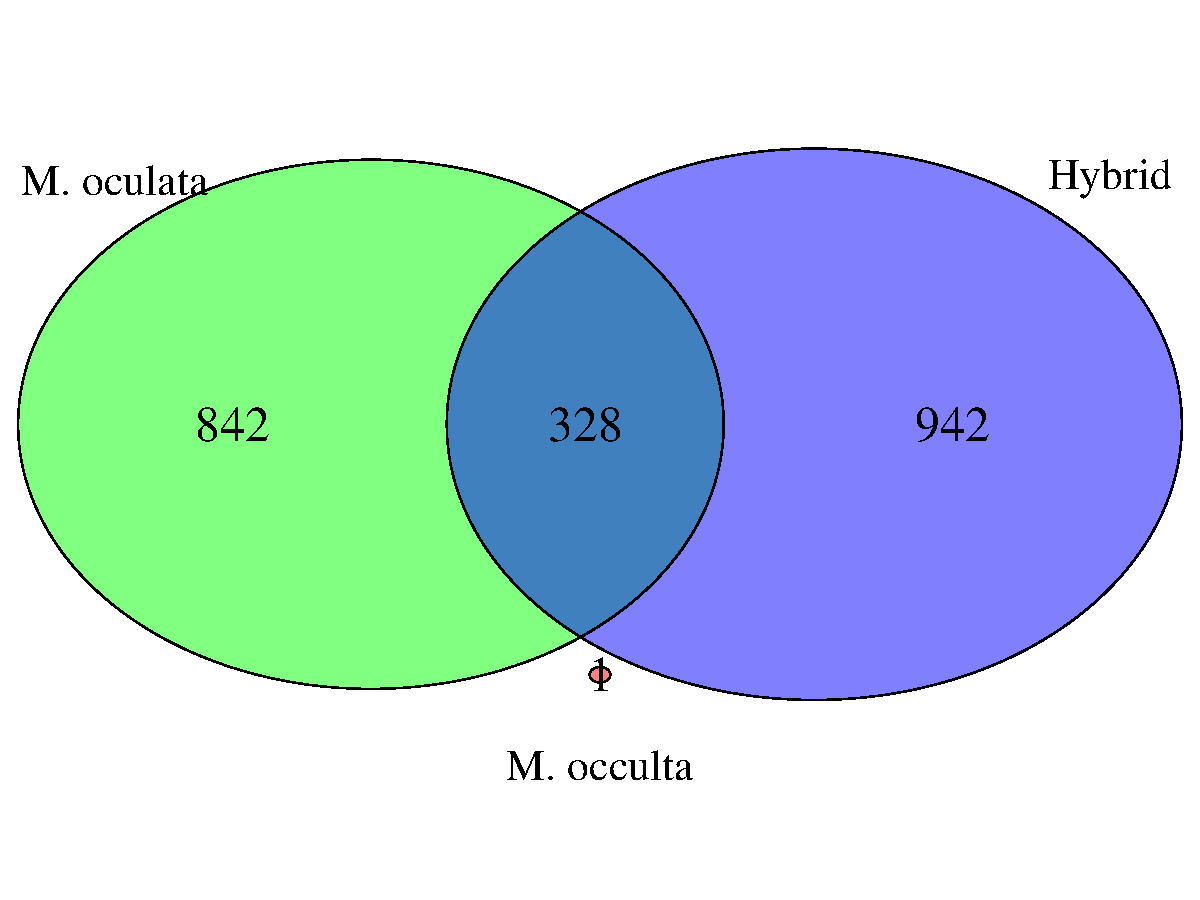
\includegraphics[width=0.45\textwidth]{figures/up_reg.pdf}
	}
	\subfloat[\label{subfig-2:overlap_allele}]{%
	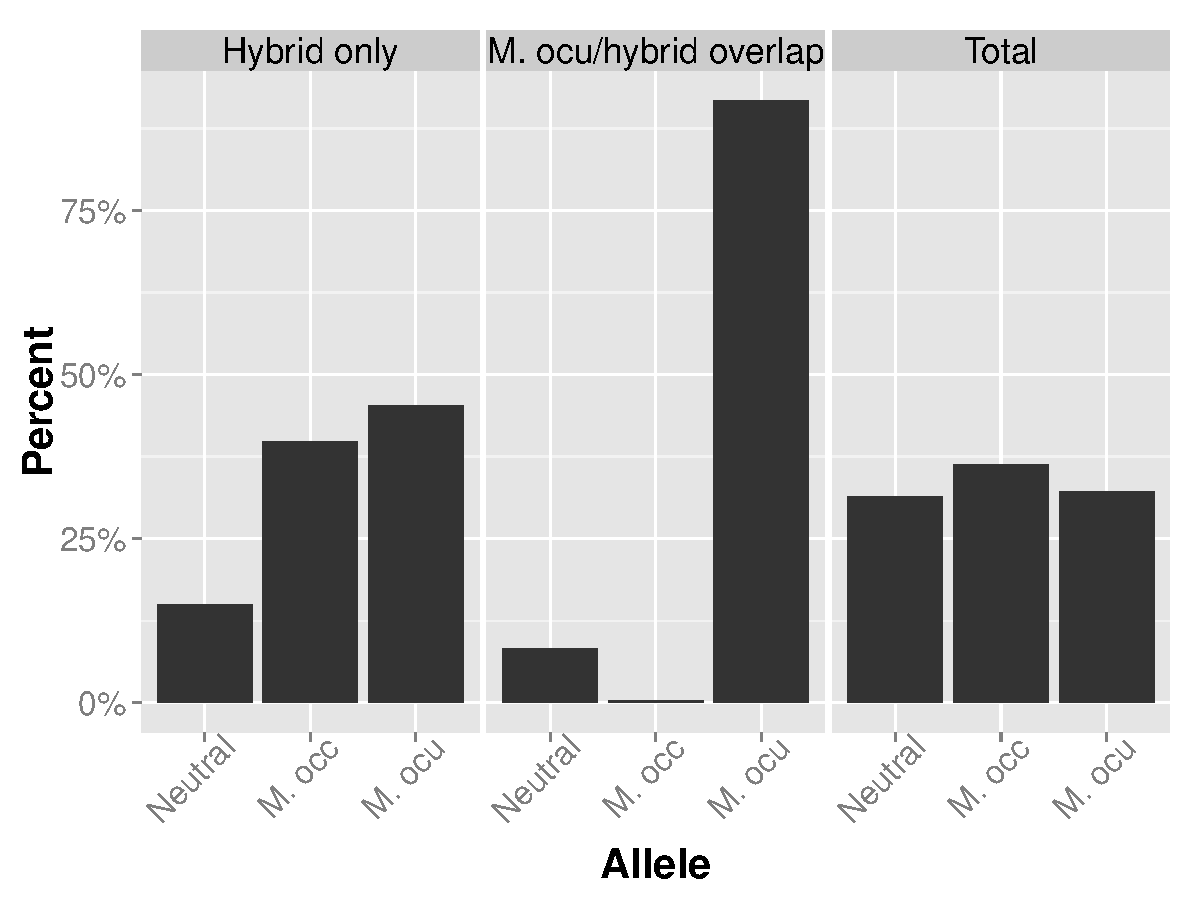
\includegraphics[width=0.45\textwidth]{figures/up_reg_allele_tb.pdf}
	}
	\caption{\textbf{Upregulated transcripts overlap between hybrid and \textit{M. oculata}.} When comparing the gastrula and neurula time point for \textit{M. occulta}, \textit{M. oculata}, and their hybrid, both \textit{M. oculata} and the hybrid showed differential expression in at least 7\% of their transcripts with the majority being up-regulated. (\ref{subfig-1:overlap}) There is a 15\% overlap in overexpressed genes \textit{M. oculata} and the hybrid, for the transcripts overexpressed when comparing gastrula to neural expression, and there is no overlap with \textit{M. occulta}. (\ref{subfig-2:overlap_allele}) When looking at the allelic express for the same condition, there is a strong skew in expression coming from the tailed allele for the unregulated transcripts that overlap between \textit{M. oculata} and the hybrid. The highest percentage of transcripts of allelic expression in the hybrid also comes from \textit{M. oculata} for up-regulated transcripts that do not overlap with \textit{M. oculata}, but not to as great an effect.  For genes' overall allelic expression, the majority comes from \textit{M. occulta}, 36\%, with 32\% coming from \textit{M. oculata}.}	
	\label{fig:upreg_tb}
\end{figure}

\section{Discussion}
Several genes identified as expressed in the notochord of \textit{C. intestinalis} \cite{hotta_characterization_2000,hotta_brachyury-downstream_2007} were observed to be missing in both \textit{M. occulta} and \textit{M. oculata}; of these genes all were also identified as being missing in the \textit{O. dioica} \cite{kugler_evolutionary_2011}. The lack of expression of these gene is the Molgulids and \textit{O. dioica} implies these genes are not necessary for the development of a fully functional notochord, CNS, or muscles in the ancestral chordate.

Here we present a differential expression analysis of two closely related \textit{Molgula} species, \textit{M. occulta} and \textit{M. oculata}, using high throughput sequencing technology. We were able to create gene models using both a mapping based approach and \textit{de novo} assembly approach, and then combined the assemblies for better transcript models. We showed that from neurula to the tailbud stage there is a 10 fold increase in transcripts that are identified as differentially expressed (p=0.05) in both \textit{M. oculata} and the hybrid. Using this same condition we were able to show that there is almost no differential expression in the the tail-less \textit{M. occulta}. This result  correlate with the embryo morphologies during this transition; in \textit{M. oculata}, the processes of tail formation are occurring, which may explain the increased transcriptional activity. In contrast in \textit{M. occulta} there are no noticeable morphological changes occurring. In hybrid embryos, this dynamic regulation of gene expression at the tailbud stage is rescued. Because hybrids show partially rescued tails and CNS structures, I propose that these transcripts may have an important role in the formation of the tail. Furthermore, of those transcripts upregulated at the tailbud stage in the hybrid but not in \textit{M. occulta}, it appears that expression is being restored from the {\em M. oculata} allele. This suggests that the relative lack of differential gene expression in the neurula-to-tailbud transition in \textit{M. occulta} may be due to loss-of-function of cis-regulatory elements controlling the expression of key genes involved in tail and CNS formation. 

\section{Conclusion}

We have used two closely related Molgulids with the ability to hybridize to study three key time points in tail development: gastrulation, neurulation and tailbud. This study has shown that from neurula to tailbud number of transcripts are up-regulated, in both \textit{M. oculata} and the hybrid. Not only are transcripts up-regulated in this condition, with no significant differential expression in the tail-less species, but there is also an overlap between the differentially expressed genes in the \textit{M. oculata} and the hybrid. Seeing that both \textit{M. occulta} and \textit{M. oculata} have a strong overlap in genes identified to be involved in notochord develop, this differential expression could be the possible cause of loss of the tail and notochord and CNS in \textit{M. occulta}. 

The hybrids shed light on the fact that cis-regulatory elements are one of the key causes for the lack of urodele features in the tai-less \textit{M. occulta}. Previously, it has been shown that \textit{Molgula} have a high turnover in sequences of cis-regulatory elements, diverging is binding sites, while keeping the orthologous gene expression \cite{stolfi_divergent_2014}. Perhaps, this cis-regulatory turnover has also led to the becoming more susceptible to the deactivation of binding sites, which in turn lead to . 
\chapter{Conclusions and Discussion}

The chordate body plan is conserved throughout the phyla with only a few species deviating from the conserved body plan; at some point in their life, most chordates develop a tadpole larvae containing a hollow dorsal neural tube, and a postanal tail containing a notochord flanked by muscle cells. However, it has been documented that 16 species out of the approximately 3000 species of tunicates\textemdash one of the three subphyla of chordates\textemdash have independently undergone tail loss, with the majority being within the molgulids \cite{berrill_studies_1931,huber_evolution_2000}. %Our work gives insight into the mechanisms behind the chordate body plan. 

Because they have both tailed and tail-less species, molgulids are useful models for studying changes in the development of body plans. Having closely related species with altered development allows us to look at the short-term modifications that occurr during the evolution of alternate body plans. This shows us that larval development can evolve rapidly. Of particular interest, two molgulids have the ability to hybridize, which allows us to examine the mechanisms of evolutionary change at an allele-specific level.

\section{Evaluating a lightweight transcriptome assembly pipeline on two closely related ascidian species}
The drop in sequencing price has aided in our efforts to understand body plan development by allowing us to quickly and inexpensively obtain transcriptome and genome sequences, along with temporal expression profiles. %Many non-model systems are now being sequenced with the drop in sequencing price. 
However, for non-model systems with no existing genomic sequence, we must first assemble the transcriptomes and genomes.  The methodology for assembly is not unambiguous: there are a number of different steps\textemdash quality trimming, filtering, and choice of assembler(s), with several programs at each step and no clear choice. Studies have been done to compare assemblers, but no one assembler is clearly the best choice \cite{clarke_comparative_2013}. Many times assembly methods are chosen on the usability of software and the availability of resources.

Factors that are most limiting for assemblies are memory, and in some cases time. The redundant nature of sequencing data allows for the removal of redundant reads with approaches like digital normalization, but at what cost? Here in efforts to assemble the first two \textit{molgula} transcriptomes, we evaluate the cost of filtering sequencing reads for redundancy. We show that abundance filtering quality trimmed assembly reads enables transcriptome assembly with a reduction in both memory requirement and assembly time, while retaining essentially the same information content (e.g. number of genes, average gene length, and homology to the closest sequence species). We have demonstrated that the Oases and Trinity assemblers return similar results, both suitable for downstream analysis using the full or redundancy filtered dataset. Our pipelines are available so we also provide methodology to be used by future researchers. In addition assembly metrics to evaluate assemblies are also an important step in the protocol. One of the standard metrics for evaluating assemblies is the N50, but this is designed for genomic evaluation and does not clearly translate to transcriptomes because of their fragmented nature, and the likelihood of chimeric contigs.  In contrast, homology and programs such as CEGMA are more informative and useful for downstream analysis, because they measure the information in the transcriptome and cover the annotation step as well. When measuring recovered homologies and CEGMA measurements we find that both assemblers and both treatments compare well. %When only taking N50 into account 
 
%The two \textit{Molgula} species that were assembled are evolutionarily interesting because of the position within the chordates and \textit{M. occulta}'s divergent body plan. The downstream analysis of these two molgula tanscriptomes will give insight into the formation of the chordate body plan. Having these transcriptomes allow us

\section{3.	Change in gene function and cis-regulatory binding sites}
In tunicates \textit{hox} genes are not important for patterning along the anterior-posterior axis, as they are in vertebrate and other bilaterians \cite{finnerty_origins_2003,mallo_regulation_2013,ikuta_limited_2010}. This limited function in the \textit{hox} genes is evident from the lack of noticeable phenotypic defects in the knockdown of \textit{C. intestinalis hox} genes, with the exception of \textit{hox10} and \textit{hox12}. \textit{Hox10} is involved in neuronal development and \textit{hox12} is involved in the formation of the posterior most portion of the the tunicate larval tail \cite{ikuta_limited_2010}. In addition, tunicates have undergone loss and rearrangement within the \textit{hox} clusters, unlike most animals that have been studied\cite{ikuta_organization_2005}. There have yet to be two tunicate species found with the same \textit{hox} cluster configuration - there are typically changes in ordering, duplications, and which hox genes are present (figure 4.2). Only \textit{C. intestinalis} has enough scaffolding to completely identify the structure and intergenic spacing between the \textit{hox} genes. However, of the \textit{hox} gene we found on the same scaffolds in \textit{M. occulta}, \textit{M. oculata} and \textit{M. occidentalis} the average intergenic spacing is far smaller than in {\em Ciona}, ranging from 10-25 kb in length. Without additionally scaffolding we cannot fully examine the rearrangements within the \textit{hox} clusters of ascidians based on the molgulid sequences. Perhaps soon after diverging from vertebrae and cephalochordates, the \textit{hox} cluster genes were co-opted into other GRNs, leading to higher lability than in species where they retained their stereotyped roles.
%inconsistency in the function of the \textit{hox} clusters was established in tunicates to conserve their highly invariant body plan and the function of the \textit{hox} genes were co-opted by other genes to establish a more robust developmental program. % leading the hox gene clusters to eventually 

We have also identified a number of enhancers between \textit{C. intestinalis}, \textit{M. occidentalis}, and \textit{M. oculata} that were either mutually unintelligible, or asymmetrically intelligible. We propose that a high frequency of compensatory changes are required for the rapidly evolving ascidians to maintain their invariant embryonic cell lineages in the presence of their compact genomes. These compensatory changes have caused the enhancers to diverge within the ascidians while allowing them to develop with their typical body plan.
% However, for this same reason the ascidians are more susceptible to undergoing a change of body plan when the frequency of compensatory changes in sequence passes an allowable threshold the binding affinity is not strong enough for the necessary protein interactions needed to drive the appropriate level of expression.

\section{Differential expression analysis of tail loss in an invertebrate chordate}
Studying closely related organisms gives us insight into the underlying evolutionary mechanisms of divergence and underlying development. Indirect and direct developing sea urchins have been studied showing that change in axial cleavage patterns and early cell fate leads to divergent larval body plans that can exhibit similar adult body plans \cite{wray_evolutionary_1989,henry_evolutionary_1990}. In contrast, ascidians retain their typical cell division and invariant cell fate in direct, indirect, tailed and tail-less ascidians \cite{jeffery_evolutionary_1991,maliska_molgula_2010}. %Next generation sequencing is a great way to study non-model species. A broad swath of information can be gained from both RNA and DNA sequencing. 
   
We have shown that evolutionary drift has occurred in the cis-regulatory modules of developing ascidian embryos between \textit{C. intestinalis} and \textit{M. occidentalis}, and these enhancers are not always capable of driving expression in other ascidian species. It appears that the same has happened between the tailed \textit{M. oculata} and tail-less \textit{M. occulta}, however those cis-mechanisms are restored in the (\textit{M. oculata x M. occulta}) interspecific hybrids, probably allowing transcription factors to bind their targets at a higher affinity and restoring the necessary level of expression to develop the urodele features. Further research is needed to identify and test cis-elements, but as of now we have a better understanding behind the mechanism of the restoration of the larval tail in hybrids, which we can at least hypothesize is driven by recovery of cis-regulatory modules.

\section{Conclusion}

When examining the tailed and tail-less \textit{Molgula}\textemdash \textit{M. oculata} and \textit{M. occulta}\textemdash there is a strong overlap (91\%) in the expression of genes that can be annotated using the \textit{C. intestinalis} proteom. There was also a strong overlap in genes associated with notochord development, which is the key structure-defining element not present in \textit{M. occulta}. We observed, it was not the lack of genes in the transcriptome, but the expression of said genes, which has led to the tail-less phenotype. So, the identification of regulatory genes expressed differently in the urodele and anural species is needed to understand the molecular mechanism underlying the evolutionary transition from urodele to anural development. Here we were able to see in the hybrids that the restored expression came from the tailed allele and we proposed that cis-regulatory modules are the cause of this. The tailed allele restored the enhancer binding sites; presumably TF were able to bind at a higher affinity and restore necessary level of expression to generate urodele features, including the formation of the notochord and hence the larval tail.

One of the shortcomings of our study is the lack of replicates from all stages; ideally we would like at least three per developmental stage for each organism. We used the available replicates to estimate the dispersion for each of the samples and because of this there are likely to be more false positives and false negatives in our analysis than there would be with more replicates. However, examining the correlation between two independent datasets, the tailed \textit{M. oculata} and the hybrid, we were able to identify a subset of genes that we believe to be differentially expressed genes. For further examination replicates are needed, along with addition sequencing of other tailed and tail-less molgula genomes and transcriptomes.  This would give us stronger insights into why the molgula are able to easily undergo tail-loss and the toolkit for molgula tail development. 

Our hypothesis depends heavily on the assumption that the gene regulatory network (GRN) is conserved within the tunicates to understand the mechanisms behind tail loss, and the GRN is conserved throughout the chordates to understand the origin the chordate body plan. Comparing the GRN of distantly related organisms can identify the genes necessary to the development of similar phenotypes and body plans. However, it is necessary to determine if the GRN have conserve structure by e.g. confirming the spatial expression patterns for the network. Next steps on this project would identify relevant transcription factors by annotating the genes and then selecting differentially expressed genes associated with DNA binding functions. Once we identify our candidate TFs we will proceed with whole mount in situ hybridization to confirm conserved spatial patterning.

As stated above, the fact that the paternal genome restores the urodele features leads us to believe that the tail loss is primarily due to a loss of function. ... in hybrids the expression of up-regulated genes involved in development of urodele features are predominately from the paternal allele. To confirm this hypothesis we would first perform a ChIP-seq analysis to identify direct binding targets, and correlate them with the differentially expressed genes.  A clear starting point is the gene \textit{bra} which is known to be important for notochord development, and \textit{Tbx2/3} which is downstream of \textit{bra}, and involved in convergence and extension.  {\em Tbx2/3} was also identified in our differential expression analysis. From this gene-targeted analysis we can examine the divergence between \textit{M. occulta} and \textit{M. oculata} enhancers, examine their binding affinities, and test the found sites using transgenesis to see if we can restore the \textit{M. occulta}'s tail.

Our hypothesis depends heavily on the assumption that the gene regulatory network (GRN) is conserved within the tunicates to understand the mechanisms behind tail loss, and the GRN is conserved throughout the chordates to understand the origin the chordate body plan. Currently we plan to expand our analysis by comparing the \textit{molgula} to the ten tunicate genomes assemblies found on the aniseed website (\url{http://www.aniseed.cnrs.fr/}), and available chordate genomes found on NCBI (\url{http://www.ncbi.nlm.nih.gov/}) and ensembl (\url{ensembl.org}). With the information we currently have we will give deeper look into the sequence divergence of both gene and non coding regions. To examine the noncoding regions addition genomic sequencing is needed for gap filling and scaffolding. Furthermore, molecularly, we will examine the spatial expression through whole mount in situ hybridization to confirm orthologous function.  Additionally we would like to identify binding sites using Chip-seq and examine the found sites using transgenesis to see if we can restore the \textit{M. occulta's} tail.


%%%%%%%    APPENDICES    %%%%%%%%%%
%% If you wish to include one appendix, remove the "%" from the 
%% following two lines.
\renewcommand{\appname}{APPENDIX}
\appendix
%\input{gloss}
\chapter{ Supplemental Figures}
%\section{k}
%\setcounter{secnumdepth}{-1}
%\thispagestyle{plain}
%\renewcommand{\thefigure}{A.\arabic{figure}}
%\setcounter{figure}{0}
\begin{figure}[thbp]
\centering
\includegraphics[scale=0.6]{figures/Hox12_13.pdf}
\caption{\textbf{Alignment for \textit{hox12-13} in \textit{M. occulta}, \textit{M. oculata} and \textit{M. occidentalis}} The contig containing \textit{hox12-13} for \textit{M. occidentalis} and \textit{M. oculata}, along with the two contigs containing \textit{hox12} and \textit{hox13} for \textit{M. occulta}. \textit{M. oculata} was used as the anchor sequence because it showed the most similarity between the three species. Outside of the coding regions and its flanking area, there is very little sequence similarity between the species, and \textit{M. occidentalis} exclusively shows similarity in coding regions. Grey arrows show the direction of the contig.}
\label{fig:hox12}
\end{figure}

\begin{figure}[thbp]
\centering
\includegraphics[scale=0.75]{figures/occi_hox2.pdf}
\caption{\textbf{Alignment of \textit{M. occidentalis} \textit{hox2} genes with \textit{Ciona} show  premature stop codon.} The \textit{M. occidentalis hox2} gene has a stop codon in the 3' region, inside of the 3/4 helix. \textit{hox2} knockdowns in \textit{Ciona} did not show any phenotypic difference, so the function of \textit{hox2} may not be important in \textit{M. occidentalis} }
\label{fig:occihox2}
\end{figure}

\begin{figure}[tbp]
\centering
\includegraphics[scale=0.75]{figures/hox_alignment.pdf}
\caption{\textbf{Alignment of \textit{hox} genes.} Alignments of the aa homeobox sequences from all the Molgula species, show that they group with their respective orthologs. All but one of the \textit{M. occidentalis} cluster properly, but \textit{M. occidentalis hox10} full homeobox sequence was not fully assembled, so this is possibly the reason for poor clustering. }
\label{fig:hox-alignments}
\end{figure}

\begin{figure}[tbp]
\centering
\includegraphics[scale=0.95]{figures/Occi_hox10.pdf}
\caption{\textbf{Alignment of \textit{M. occidentalis} duplicate \textit{hox10} genes} Two copies of \textit{hox10} were found in \textit{M. occidentalis} \mytilde12 kb apart on the same contig.}
\label{fig:occihox10}
\end{figure}

\begin{figure}[tbp]
\centering
\includegraphics[scale=0.10]{figures/gel.jpg}
\caption{\textbf{Gel electrophoresis of cdc45, netrin and controls} \textit{Netrin} was not found in \textit{M. occulta's} transcriptome but was recovered via PCR from a cDNA library. However, this library has a wider range of developmental stages, so it is still possible \textit{netrin} is not expressed at the right stage for tail development.}
\label{fig:gel}
\end{figure}

\begin{figure}[tbp]
\centering
\includegraphics[scale=0.55]{figures/prickle.pdf}
\caption{\textbf{Whole Mount In Situ Hybridization of \textit{prickle} in \textit{M. occulta}} The PCP gene \textit{pk} was shown to be expressed in the notochord in a similar pattern to \textit{C. intestinalis} }
\label{fig:prickle}
\end{figure}

%% To include several appendices, remove the only the "%"
%% in front of "\appendix".

%% In either cast to start your first appendix, which will be labeled
%% as Appendix A, just type \chapter{<appendix 1 name>}
%% and enter the text of the appendix as you would a chapter.

%%%%%%% A NOTE ABOUT APPENDICES %%%%%%%%%
%% Some appendices may be single spaced such as survey examples or letters.
%% Contact the Graduate School for details.
%% To single space an appendix first remove the % from 
%% the following two lines. 
% \end{doublespace}
% \chapter{<appendix  name>}
%% After entering the appendix remove the % from 
%% the following line
 %\begin{doublespace}
%% Any text entered now will be double spaced.
\end{doublespace}

%%Bibliography 

%% A bibliography is required. By default it is called, "Bibliography"
%% You may use �Literature Cited�, �Works Cited� or �References� 
%% instead of �Bibliography� if that is the convention in your discipline. 
%% To do so, place your choice in the  empty argument 
%% of the following command and remove the "%".
\renewcommand{\bibname}{BIBLIOGRAPHY}
%% The bibliography may be made using BibTeX.
%% If it's made from scratch,
%% remove the "%" in front of "\begin{thebibliography}{???}"
%% replacing the ??? with the appropriate entry and 
%% remove the "%" in front of "\end{thebibliography}"
%\begin{thebibliography}{MyLibrary}
%%  Enter the bibliography here.
%\end{thebibliography}

\bibliographystyle{abbrv}
\bibliography{MyLibrary}

\end{document}
